\documentclass[
    % -- opções da classe memoir --
    12pt,                % tamanho da fonte
    %openright,            % capítulos começam em pág ímpar (insere página vazia caso preciso)
    oneside,            % twoside para impressão em verso e anverso. Oposto a oneside
    a4paper,            % tamanho do papel.
    % -- opções da classe abntex2 --
    %section=TITLE,        % títulos de capítulos convertidos em letras maiúsculas
    %section=TITLE,        % títulos de seções convertidos em letras maiúsculas
    %subsection=TITLE,    % títulos de subseções convertidos em letras maiúsculas
    %subsubsection=TITLE,% títulos de subsubseções convertidos em letras maiúsculas
    % -- opções do pacote babel --
    english,            % idioma adicional para hifenização
    french,                % idioma adicional para hifenização
    spanish,            % idioma adicional para hifenização
    brazil                % o último idioma é o principal do documento
    ]{abntex2}

% ---
% Pacotes básicos
% ---
\usepackage{lmodern}            % Usa a fonte Latin Modern            
\usepackage[T1]{fontenc}        % Selecao de codigos de fonte.
\usepackage[utf8]{inputenc}        % Codificacao do documento (conversão automática dos acentos)
\usepackage{indentfirst}        % Indenta o primeiro parágrafo de cada seção.
\usepackage{lastpage}            % Usado pela Ficha catalográfica

\usepackage{color}                % Controle das cores
%\usepackage[demo]{graphicx}
\usepackage{graphicx}            % Inclusão de gráficos
\usepackage{microtype}             % para melhorias de justificação
\usepackage{amsmath}


\usepackage[position=bottom]{subfig}
%\usepackage[hang]{subfigure}
%\usepackage{subfigure}

%\usepackage[utf8]{inputenc}
\usepackage{algorithm}
%\usepackage{algorithm2e}

\makeatletter
\renewcommand{\ALG@name}{Algoritmo}
\makeatother
\renewcommand{\listalgorithmname}{Lista de Algoritmos}

\usepackage[brazil]{babel}
\usepackage[justification=centering]{caption}

% adicionado por Ting
\setlength{\marginparwidth}{2cm}
\usepackage{todonotes}
%\usepackage{soul}
\usepackage[normalem]{ulem}
\usepackage{hyperref}

%\setlength\afterchapskip{\lineskip}




% ---
        
% ---
% Pacotes adicionais, usados apenas no \^{a}mbito do Modelo Can\^{o}nico do abnteX2
% ---
\usepackage{lipsum}				% para gera\c{c}\~{a}o de dummy text
\usepackage{nomencl}
\usepackage{amsmath}
\usepackage{bbm}
\usepackage{multirow}
\usepackage{rotating}
\usepackage{pdfpages}
%\usepackage[font=footnotesize]{subfig}
\usepackage{booktabs}
\usepackage{pdflscape}
\usepackage{chngcntr}

\usepackage{algpseudocode,algorithm}


%\let\printglossary\relax
%\let\theglossary\relax
%\let\endtheglossary\relax

\usepackage[nonumberlist,acronym,nomain]{glossaries} % nonnumberlist nao mostra as paginas nas quais os acronimos aparecem no texto
%\newglossary[tlg]{simbolos}{tld}{tdn}{Lista de símbolos}
% Generate the glossary
%\makeglossaries


\counterwithin{figure}{chapter}
\counterwithin{table}{chapter}
% Pacotes de citações
% ---
\usepackage[brazilian,hyperpageref]{backref}     % Paginas com as citações na bibl
\usepackage[alf]{abntex2cite}    % Citações padrão ABNT

\usepackage{unicamp}

% ---
% CONFiguraÇÕES DE PACOTES
% ---

% ---
% ConFigurações do pacote backref
% Usado sem a opção hyperpageref de backref
\renewcommand{\backrefpagesname}{Citado na(s) página(s):~}
% Texto padrão antes do número das páginas
\renewcommand{\backref}{}
% Define os textos da citação
\renewcommand*{\backrefalt}[4]{
    \ifcase #1 %
        Nenhuma citação no texto.%
    \or
        Citado na página #2.%
    \else
        Citado #1 vezes nas páginas #2.%
    \fi}%
% ---

%Redefinições de comando para pseudocódigo - Portugues
% Declaracoes em Português
%\algrenewcommand\algorithmicend{\textbf{fim}}
%\algrenewcommand\algorithmicdo{\textbf{faça}}
%\algrenewcommand\algorithmicwhile{\textbf{enqua%nto}}
%\algrenewcommand\algorithmicfor{\textbf{para}}
%\algrenewcommand\algorithmicif{\textbf{se}}
%\algrenewcommand\algorithmicthen{\textbf{então}%}
%\algrenewcommand\algorithmicelse{\textbf{senão}%}
%\algrenewcommand\algorithmicreturn{\textbf{devo%lve}}
%\algrenewcommand\algorithmicfunction{\textbf{fu%nção}}
%
%% Rearranja os finais de cada estrutura
%\algrenewtext{EndWhile}{\algorithmicend\ %\algorithmicwhile}
%\algrenewtext{EndFor}{\algorithmicend\ %\algorithmicfor}
%\algrenewtext{EndIf}{\algorithmicend\ %\algorithmicif}
%\algrenewtext{EndFunction}{\algorithmicend\ %\algorithmicfunction}
%
%% O comando For, a seguir, retorna 'para #1 -- %#2 até #3 faça'
%\algnewcommand\algorithmicto{\textbf{até}}
%\algrenewtext{For}[3]%
%{\algorithmicfor\ #1 $\gets$ #2 \algorithmicto\ %#3 \algorithmicdo}

% ---


% ---
% Informações de dados para CAPA e FOLHA DE ROSTO
% ---

%\tipotrabalho{Relatório de Qualificação de Mestrado}
% O preambulo deve conter o tipo do trabalho, o objetivo,
% o nome da instituição e a área de concentração

% ---


% ---
% Configurações de aparência do PDF final

% alterando o aspecto da cor azul
\definecolor{blue}{RGB}{41,5,195}

% informações do PDF
\makeatletter
\hypersetup{
         %pagebackref=true,
        pdftitle={\@title},
        pdfauthor={\@author},
        pdfsubject={\imprimirpreambulo},
        pdfcreator={LaTeX with abnTeX2},
        pdfkeywords={abnt}{latex}{abntex}{abntex2}{trabalho acadêmico},
        colorlinks=true,               % false: boxed links; true: colored links
        linkcolor= blue,              % color of internal links
        citecolor=blue,                % color of links to bibliography
        filecolor=magenta,              % color of file links
        urlcolor=blue,
        bookmarksdepth=4
}
\makeatother
% ---

% ---
% Espaçamentos entre linhas e parágrafos
% ---

% O tamanho do parágrafo é dado por:
\setlength{\parindent}{2cm}

% Controle do espaçamento entre um parágrafo e outro:
\setlength{\parskip}{0.2cm}  % tente também \onelineskip

\setlength\afterchapskip{\lineskip}

\titulo{\textcolor{red}{????Tractografia baseada em Q-Ball Imaging e análise da reconstrução do trato corticoespinhal????}}
\autor{Daniel Xavier Silva}
\orientador{Profa. Dra. Wu Shin-Ting}
\local{Campinas}
\data{2021}
\instituicao{%
  UNIVERSIDADE ESTADUAL DE CAMPINAS
    \par
    Faculdade de Engenharia Elétrica e de Computação
  %Departamento de Engenharia de Computação e Automação Industrial - DCA\par
  %Faculdade de Engenharia Elétrica e de Computação - FEEC
  }
  \tipotrabalho{Dissertação (Mestrado)}
  \preambulo{Dissertação apresentada à Faculdade de Engenharia Elétrica e de Computação da Universidade Estadual de Campinas como parte dos requisitos exigidos para a obtenção do título de Mestre em Engenharia Elétrica, na Área de Engenharia de Computação.}

% ---
% compila o indice
% ---
\makeindex
% ---

% ----
% Início do documento
% ----

\begin{document}



% ----------------------------------------------------------
% ELEMENTOS PRÉ-TEXTUAIS
% ----------------------------------------------------------
% \pretextual

% ---
% Capa
% ---
% ---

\imprimircapa
% ---
% Folha de rosto
% (o * indica que haverá a ficha bibliográfica)
% ---
\imprimirfolhaderosto*
% ---

% ---
% Inserir a ficha bibliografica
% ---
\begin{fichacatalografica}
    \vspace*{\fill}
    \begin{center}
        \textsc{Inclua aqui o pdf com a ficha catalogr\'{a}fica fornecida pela BAE.}
    \end{center}
    \vspace*{\fill}
    %\includepdf{fig_ficha_catalografica.pdf}
\end{fichacatalografica}

% Isto é um exemplo de Ficha Catalográfica, ou ``Dados internacionais de
% catalogação-na-publicação''. Você pode utilizar este modelo como referência.
% Porém, provavelmente a biblioteca da sua universidade lhe fornecerá um PDF
% com a ficha catalográfica definitiva após a defesa do trabalho. Quando estiver
% com o documento, salve-o como PDF no diretório do seu projeto e substitua todo
% o conteúdo de implementação deste arquivo pelo comando abaixo:
%
% \begin{fichacatalografica}
%     \includepdf{fig_ficha_catalografica.pdf}
% \end{fichacatalografica}
% \begin{fichacatalografica}
%     \vspace*{\fill}                    % Posição vertical
%     \hrule                            % Linha horizontal
%     \begin{center}                    % Minipage Centralizado
%     \begin{minipage}[c]{12.5cm}        % Largura
    
%     \imprimirautor
    
%     \hspace{0.5cm} \imprimirtitulo  / \imprimirautor. --
%     \imprimirlocal, \imprimirdata-
    
%     \hspace{0.5cm} \pageref{LastPage} p. : il. (algumas color.) ; 30 cm.\\
    
%     \hspace{0.5cm} \imprimirorientadorRotulo~\imprimirorientador\\
    
%     \hspace{0.5cm}
%     \parbox[t]{\textwidth}{\imprimirtipotrabalho~--~\imprimirinstituicao,
%     \imprimirdata.}\\
    
%     \hspace{0.5cm}
%         1. Palavra-chave1.
%         2. Palavra-chave2.
%         I. Orientador.
%         II. Universidade xxx.
%         III. Faculdade de xxx.
%         IV. Título\\             
    
%     \hspace{8.75cm} CDU 02:141:005.7\\
    
%     \end{minipage}
%     \end{center}
%     \hrule
% \end{fichacatalografica}


% \includepdf{folhadeaprovacao_final.pdf}
%
% --- Inserir folha de aprova\c{c}\~{a}o ---

% Isto \'{e} um exemplo de Folha de aprova\c{c}\~{a}o, elemento obrigat\'{o}rio da NBR
% 14724/2011 (se\c{c}\~{a}o 4.2.1.3). Voc\^{e} pode utilizar este modelo at\'{e} a aprova\c{c}\~{a}o
% do trabalho. Ap\'{o}s isso, substitua todo o conte\'{u}do deste arquivo por uma
% imagem da p\'{a}gina assinada pela banca com o comando abaixo:
%
% \begin{folhadeaprovacao}
% \includepdf{folhadeaprovacao_final.pdf}
% \end{folhadeaprovacao}
%
\begin{folhadeaprovacao}

  \begin{center}
    COMISS\~{A}O JULGADORA - TESE DE DOUTORADO
    %\textsc{Inclua aqui a folha de assinaturas.}
\end{center}
\noindent
\begin{minipage}{\textwidth}\SingleSpacing
Candidato(a): Nome do Autor      RA: XXXXXX

Data de defesa: XX de MES de 202X

T\'{i}tulo da Tese: "XXXXXXXXXXXXXXXXXXXXXXXXXXXXXXX"
\vspace{2cm}

Profa. Dra. Xxxxxxxxxx (Presidente)

Profa. Dra. xxxxxxx

Profa. Dra. xxxxxxx

Profa. Dra. xxxxxxxxx

Profa. Dra xxxxxxxxxxxx

\vspace{2cm}

A Ata de Defesa, com as respectivas assinaturas dos membros da Comissão Julgadora, encontra-se no SIGA (Sistema de Fluxo de Dissertação/Tese) e na Secretaria de Pós-Graduação da Faculdade de Engenharia Elétrica e de Computação.
\end{minipage}

\end{folhadeaprovacao}
% ---

% ---
% Dedicatória
% ---
\begin{dedicatoria}
   \vspace*{\fill}
   \centering
   \noindent
   \textit{!!Eu dedico este trabalho} \vspace*{\fill}
\end{dedicatoria}
% ---

% ---
% Agradecimentos
% ---
% ---
\begin{agradecimentos}
    !!O presente trabalho foi realizado com apoio do CNPq, Conselho Nacional de Desenvolvimento Científico  e Tecnológico – Brasil.
\end{agradecimentos}

% ---
% Epígrafe
% ---
\begin{epigrafe}
    \vspace*{\fill}
	\begin{flushright}
		\textit{``Escreva aqui a sua ep\'{\i}grafe (Opcional)''\\
		(Cita\c{c}\~{a}o)}
	\end{flushright}
\end{epigrafe}
% ---

% ---
% RESUMOS

%% resumo em português
\setlength{\absparsep}{18pt} % ajusta o espaçamento %dos parágrafos do resumo
\begin{resumo}

A ressonância magnética ponderada por difusão (DWI) é uma sequência de imageamentos que mensura informações direcionais de difusão de fluidos. Aplicada ao cérebro, o DWI é único no que diz respeito à quantificação deste fenômeno em tecido vivo, o que possibilita a inferência da arquitetura de matéria branca do cérebro \textit{in-vivo} e de forma não-invasiva, conhecida por tractografia. Algoritmos de tractografia consistem na extração de informações direcionais de dados coletados por DWI e aplicá-las na reconstrução de fibras cerebrais. A técnica de tractografia por tensor de difusão (DTI) é a mais conhecida e difundida clinicamente. No entanto, há falhas na reconstrução, especialmente em regiões onde coexistem várias fibras, o que é algo muito evidenciado na literatura da área. Face a este problema, este trabalho visa: investigar o método Q-Ball, que modela a difusão como uma função de distribuição de orientações (ODF), um esquema de visualização de ODFs em tempo interativo através de glifos e a implementação de um algoritmo tractografia a partir de potenciais direções extraídas do modelo.

\vspace{\onelineskip}
\noindent\textbf{Palavras-chave}: Q-Ball Imaging, HARDI, ressonância magnética ponderada por difusão, renderização de glifos, tractografia
\end{resumo}
\pagebreak
%
%% resumo em inglês
\begin{resumo}[Abstract]
 \begin{otherlanguage*}{english}
A ressonância magnética ponderada por difusão (DWI) é uma sequência de imageamentos que mensura informações direcionais de difusão de fluidos. Aplicada ao cérebro, o DWI é único no que diz respeito à quantificação deste fenômeno em tecido vivo, o que possibilita a inferência da arquitetura de matéria branca do cérebro \textit{in-vivo} e de forma não-invasiva, conhecida por tractografia. Algoritmos de tractografia consistem na extração de informações direcionais de dados coletados por DWI e aplicá-las na reconstrução de fibras cerebrais. A técnica de tractografia por tensor de difusão (DTI) é a mais conhecida e difundida clinicamente. No entanto, há falhas na reconstrução, especialmente em regiões onde coexistem várias fibras, o que é muito evidenciado na literatura da área. Face a este problema, este trabalho visa: investigar o método Q-Ball, que modela a difusão como uma função de distribuição de orientações (ODF), um esquema de visualização de ODFs em tempo interativo através de glifos e a implementação de um algoritmo tractografia a partir de potenciais direções extraídas do modelo.

\vspace{\onelineskip}
\noindent\textbf{Palavras-chave}: QBall Imaging, HARDI, ressonância magnética ponderada por difusão, renderização de glifos, tractografia
 \end{otherlanguage*}
\end{resumo}


% ---
% inserir lista de ilustrações
% ---
\pdfbookmark[0]{\listfigurename}{lof}
\listoffigures*
\cleardoublepage
% ---

% ---
% inserir lista de tabelas
% ---
\pdfbookmark[0]{\listtablename}{lot}
\listoftables*
\cleardoublepage
% ---

% ---
% inserir lista de abreviaturas e siglas
% ---
\begin{siglas}
\item[DWI] \textit{Diffusion Weighted Magnetic Resonance Imaging} (Ressonância Magnética Ponderada por Gradientes de Difusão)
  
\item[DTI] \textit{Diffusion Tensor Imaging}(Imageamento por Tensor de Difusão)

\item[HARDI] \textit{High Angular Resolution DiffusionImaging} (Imageamento de difusão por alta resolução angular)

\item[FA] \textit{Fractional Anisotropy} (Anisotropia Fracionada)

\item[QBI] \textit{Q-Ball Imaging}

\item[MRI] Magnetic Resonance Imaging (Imageamento por Ressonância Magnética)

\item[CST] \textit{Corticospinal Tract} (Trato Corticoespinhal)

\item[GQI] \textit{Generalized Q-Sampling Imaging} (amostragem generalizada no espaço Q)

\item[ROI] \textit{Region of Interest} (Região de Interesse)

\item[ODF] \textit{Orientation Distribution Function} (Função de Distribuição de orientação)

\item[!!fODF] !não esquecer desse aqui

\item[ISMRM]    \textit{International Society for Magnetic Resonance in Medicine} (Sociedade Internacional para Ressonância Magnética em Medicina)

\item[UNICAMP] Universidade Estadual de Campinas

\item[SLF] \textit{Superior Longitudinal Fasciculus} (Fascículo Longitudinal Superior)

\item[CC] Corpo Caloso

\item[GFA] \textit{Generalized Fractional Anisotropy} Anisotropia Fracionada Generalizada

\item[DSI] \textit{Diffusion Spectrum Imaging} (Imagemento por Espectro de difusão)

\item [CPU] \textit{Computer Processing Unit} (Unidade de Processamento Computacional)

\item [GPU] \textit{Graphics Processing Unit} (Unidade de Processamento Gráfico)
\end{siglas}


% ---

% ---
% inserir lista de símbolos
% ---

% ---

% ---
% inserir o sumario
% ---
\pdfbookmark[0]{\contentsname}{toc}
\tableofcontents*
\cleardoublepage
% ---



% ----------------------------------------------------------
% ELEMENTOS TEXTUAIS
% ----------------------------------------------------------
\textual



\chapter{Introdução}
\label{sec:introducao}

A difusão molecular é um processo físico que se refere ao movimento aleatório de moléculas de fluídos que resultam da sua energia térmica \cite{lebihan2006}. 
Pode-se categorizar o movimento de difusão em relação ao meio da sua ocorrência em difusão isotrópica e anisotrópica. A difusão isotrópica ocorre em um meio que não oferece obstáculos, enquanto na difusão anisotrópica, o meio apresenta restrições ao movimento.

No cérebro, o processo de difusão ocorre majoritariamente com moléculas de água e difere significantemente da difusão isotrópica \cite{lebihan2006}. As moléculas interagem com muitos dos tecidos cerebrais, como membranas de células e fibras. Estas interações reduzem e restringem a distância da difusão.


Há diferenças na forma de ocorrência da difusão nas substâncias branca e cinzenta do cérebro. Na substância cinzenta, a característica da difusão é altamente complexa devido à sua organização em camadas, o que torna a interpretação do fenômeno bem desafiadora. A substância branca, por sua vez, é composta por fibras organizadas em um conjunto coerente e compactado que faz a conexão entre neurônios localizados em diferentes partes do cérebro, o que faz a difusão ter um comportamento proeminente ao longo da direção do feixe de fibras \cite{DTI_Handbook}.

\todo{Por quê}A medição das características difusão da água no cérebro pode fornecer informações sobre a matéria branca, que se referem a direção de fibras e conectividade do cérebro. Esta medição é possível através da ressonância magnética ponderada por difusão (\textit{diffusion-weighted magnetic resonance imaging} - DW-MRI ou DWI).

%O DWI é uma forma de ressonância magnética que gera contraste a partir da difusão das moléculas de água em determinadas direções \cite{DTI_Handbook}. %A partir do sinal adquirido, há ferramentas que  possibilitam o seu mapeamento em  fibras nervosas do cérebro humano \textit{in-vivo}.

%A ressonância magnética ponderada na sequência de difusão (\textit{diffusion-weighted magnetic resonance imaging} - DW-MRI ou DWI) é uma sequência de ressonância magnética que mensura a difusão das moléculas de água em determinadas direções \cite{DTI_Handbook}. A partir do sinal adquirido, há ferramentas que  possibilitam o seu mapeamento em  fibras nervosas do cérebro humano \textit{in-vivo}.

%!!A forma mais comum para gerar o DWI é através da sequência e pulsos PGSE (\textit{Pulsed Gradient Spin Echo}).


Na aquisição do DWI, é escaneado um conjunto de volumes em que cada um possui a ponderação de único gradiente de difusão associado a um valor-b\footnote{O valor-b é uma métrica de sensitividade para difusão e é função de parâmetros da aquisição do DWI, como função da intensidade, duração e o intervalo de tempo dos gradientes de ponderação de difusão. Quanto maior o seu valor, maior o decaimento do sinal relativo à difusão.}, e, adicionalmente, um ou mais volumes sem ponderação de gradiente, denominado volume b0. A quantidade de volumes ponderados para diferentes direções de gradiente é denominada de resolução angular. Técnicas para sumarizar os sinais coletados em informações de potenciais caminhos de fibras nervosas são objeto de pesquisa desde o início dos anos 90 \cite{descoteaux2015}.%\sout{há mais de 25 anos}\textcolor{red}{desde os primeiros trabalhos seminais ...}.

O método de imageamento mais amplamente utilizada para estes fins é chamada de imageamento por tensor de difusão (DTI - \textit{Diffusion Tensor Imaging}), proposto por \citeonline{Basser1994}. 

O método do DTI consiste em um mapeamento das amostras de difusão em um ponto contido em uma aquisição DWI em um modelo gaussiano, que é sintetizada por tensor de ordem 2, representado por uma matriz 3x3 simétrica. A informação referente ao processo de difusão é comumente extraída dos seus três autovetores e autovalores.%  do tensor de difusão representam três direções ortogonais cujos respectivos autovalores representam a magnitude de difusão, que são máximos para restrição de ortogonalidade.

%\todo[inline]{Abstraindo o que você escreveu ... há duas linhas de empenho: visualização dos sinais de difusão por amostra (modelagem local da geometria das fibras) e/ou por fibra (modelagem global da conectividade das amostras). É melhor colocar Fig 1.1 e 1.2 uma ao lado da outra. Facilita análise comparativa.}
Há pesquisas na área de visualização de volumes DWIs, tanto no que diz respeito à criação de glifos representativos do comportamento de difusão, quanto à reconstrução das fibras do cérebro -- denominada tractografia.

\citeonline{Basser1994} e \citeonline{Kindlmann2004}, por exemplo, propuseram glifos representativos que sintetizam a difusão a partir do DTI. Na figura \ref{fig::intro_ex_DTI_glifos} ilustra glifos propostos por os glifos propostos por \citeonline{Kindlmann2004}, denominados superquádricos.

As fibras reconstruídas consistem de informações direcionais extraídas de um método de imageamento e costumam ser representadas por linhas, como ilustrado na figura \ref{fig::intro_ex_DTI_tractografia}. Algoritmos de tractografia baseados em DTI são exemplificados por \citeonline{Weinstein1999} e \citeonline{basser2000}. 

\begin{figure}[ht]
\captionsetup[subfloat]{farskip=0pt,nearskip=0pt}
    \subfloat[Tensores de difusão representado por glifos superquádricos em uma fatia axial do cérebro na região do corpo caloso. As cores representam a direção predominante de difusão onde vermelho é esquerda-direita, azul é superior-inferior e verde é anterior-posterior]{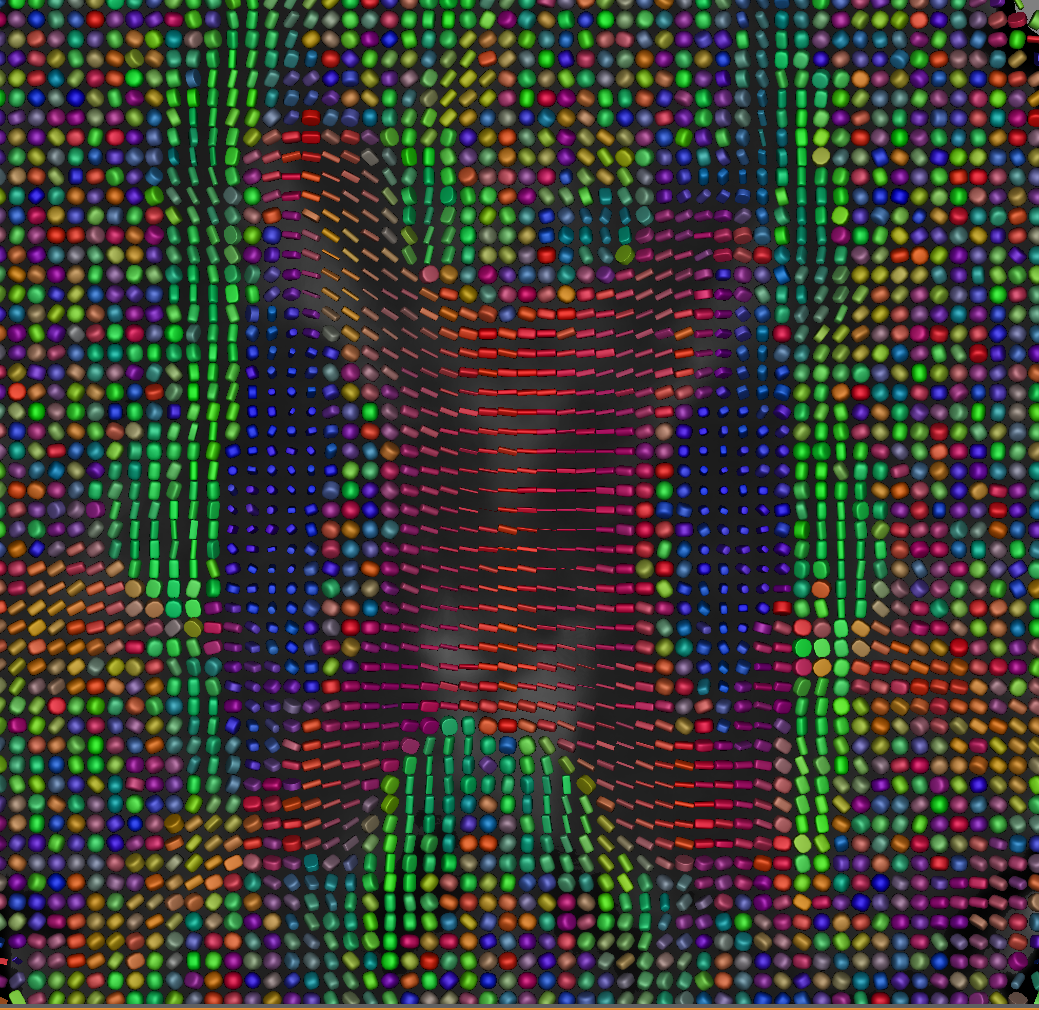
\includegraphics[width=.52\linewidth, angle=0]{figs/Introducao/ex_DTI_Superquadrica.png}
    \label{fig::intro_ex_DTI_glifos}}
    \hfill
    \subfloat[Trato fascículo inferior fronto-occipital (IFOF). A cor predominantemente verde indica sua trajetória, que ocorre na direção anterior-posterior. As linhas são reconstruídas com base no proposto por \citeonline{Weinstein1999} ]{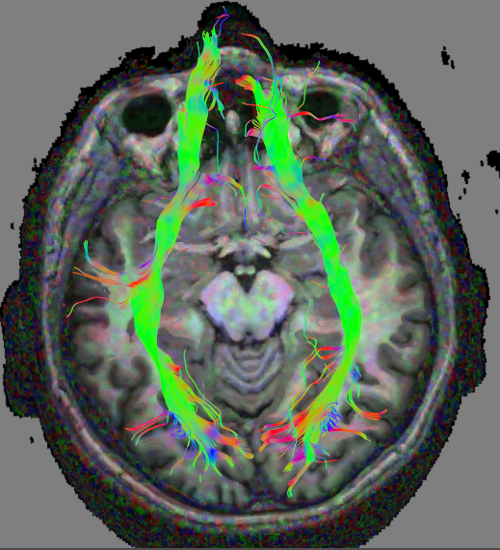
\includegraphics[width=.46\linewidth, angle=0]{figs/Introducao/ex_DTI_tractography.png}
    \label{fig::intro_ex_DTI_tractografia}}
    \hfill
    \label{fig::intro_ex_DTI}
\end{figure}

%\begin{figure}[ht]
%
%\centering
%\includegraphics[width=.485\linewidth, %angle=00]{figs/Introducao/ex_DTI_Superquadric%a.png}
%\centering
%\caption{Tensor de difusão representado por %glifos superquádricos em uma fatia axial do %cérebro na região do corpo caloso. As cores %representam a direção predominante de difusão %onde vermelho é esquerda-direita, azul é %superior-inferior e verde é %anterior-posterior}
%\label{fig::intro_ex_DTI_Superquadrica}
%\end{figure}

%\begin{figure}[ht]
%\centering
%\includegraphics[width=.485\linewidth, %angle=00]{figs/Introducao/ex_DTI_tractography%.png}
%\caption{Trato fascículo inferior %fronto-occipital (IFOF). A cor %predominantemente verde indica sua %trajetória, que ocorre na direção %anterior-posterior}
%\label{fig::intro_ex_DTI_Tractografia}
%\hfill
%\end{figure}

Em tractografia, devido a sua natureza de modelagem, o DTI apresenta limitações. O modelo gaussiano usado no DTI descreve bem regiões de fibras em que o comportamento de difusão ocorre predominantemente em uma direção. Em pontos que contém múltiplas fibras e que estão dispostas nas mais variadas configurações (por exemplo: cruzamento, bifurcação, mistura, "beijo") o modelo gaussiano não sintetiza de forma correta o comportamento da difusão, impedindo o cômputo das direções plausíveis para reconstrução de uma fibra de interesse \cite{fillard2011, daducci2014}. Há um estimativa que entre 66\% a 90\% da substância branca do cérebro contém múltiplas configurações de cruzamento de fibra \cite{descoteaux2015} e a limitação do DTI é um obstáculo para traçar o caminho de fibras do cérebro de forma efetiva.


%\section{Motivação}
%\label{ssec:motivation}

Cientes das limitações do DTI, pesquisadores da área passaram a propor modelos matemáticos mais descritivos do processo de difusão, bem como aplicar estes modelos a volumes de alta resolução angular  (HARDI - \textit{High Angular Resolution Diffusion Imaging}). A tese de doutorado de David Tuch \cite{tuch2002} é o trabalho seminal da área.

Uma aquisição DWI é considerada HARDI se há 45 ou mais gradientes de ponderação de difusão. Esta modalidade de aquisição se diferencia de uma aquisição DTI, que costuma possuir entre 6 a 32 direções \cite{descoteaux2015}.


%\todo{\url{https://www.researchgate.net/figure/Sampling-schemes-in-q-space-a-Cartesian-sampling-dedicated-to-diffusion-spectrum_fig3_319558026}}.
Para aquisições HARDI, foram propostos métodos de imageamento mais descritivos do processo de difusão que o DTI. Alguns deles consistem na abordagem multi-tensor \cite{tuch2002}, o \textit{Q-Ball Imaging} (QBI) \cite{tuch2002, Kindlmann2004}, \textit{constrained spherical deconvolution} (CSD) \cite{tournier2007}, \textit{diffusion spectrum imaging} (DSI) \cite{tuch2002,wedeen2005} e a amostragem generalizada do espaço Q (GQI - \textit{generalized Q-space sampling}) \cite{yeh2010}. Os métodos consistem no cômputo de uma função de distribuição de orientação (ODF - \textit{orientation distribution function}), no qual padrões de fibras subjacentes podem ser inferidos. Para diferenciá-los do DTI, neste trabalho chamaremos estes métodos de imageamento de métodos HARDI.

A partir de volumes com mais alta resolução angular e métodos HARDI, é possível gerar algoritmos de tractografia melhores e que levem em consideração mais nuances do sinal de difusão que o DTI, especialmente em regiões que contém as mais diversas configurações de múltiplas de fibras \cite{fillard2011}. Porém, aquisições e métodos HARDI não são popularmente utilizadas clinicamente. %\textcolor{red}{Porém, (comentar o que falta ainda para popularizar o seu uso clínico em relação a DTI) ...}

No uso clínico, o DTI é ainda muito mais utilizado que métodos HARDI \cite{descoteaux2015}. As vantagens do DTI se referem a sua aquisição, que requer menos tempo para ser feita e a popularidade de aplicativos que processam DWI por este método de imageamento. O DTI demanda uma menor quantidade memória para armazenar parâmetros intrínsecos ao seu método comparados aos métodos HARDI e suas ferramentas para análise de DWIs são computacionalmente menos exigentes.

%Falar de tratos que HARDI resolve e DTI não?

Em tractografia, tanto baseada em DTI, quanto HARDI, há avanços no entendimento de patologias, como esclerose múltipla, mal de Parkinson, esquizofrenia e derrame \cite{SCHILLING2019194}. Mesmo com essas aplicabilidades, há muitos desafios na área.

Mesmo métodos HARDI conseguindo sanar os problemas já citados do DTI, há muitos desafios na área. Mesmo sendo precisos na detecção de orientação local, não inferem sobre a configuração de fibras. Por exemplo, se em um ponto, há duas ou mais direções de fibras, o método irá identificá-las, mas o mesmo não infere sobre a configuração de ambas (por exemplo, se as fibras se cruzam ou se "beijam") \cite{SCHILLING2019194}.

%%RELER O ARTIGO DO SCHILING E MOSTRAR OPORTUNIDADES 



\todo[inline]{Sugiro mencionar aqui o artigo de Schilling et al. mostrando os desafios ainda em aberto.}

\section{Motivação}
\label{ssec:motivation}

Diante dos desafios em aberto, este trabalho aborda um sistema de visualização interativa para dados de difusão HARDI, utilizando um método de imageamento apropriado.

O sistema proposto tem a intenção de ser usado por um especialista para que, a partir de um DWI, ele possa construir e analisar de forma não invasiva fibras dos cérebros. Para este fim, iremos propor a visualização interativa de perfis de difusão gerados pelo método de imageamento utilizado e um algoritmo de tractografia interativo associado.

A visualização interativa de perfis de difusão em cada amostra dá ao especialista uma visão de como o método utilizado o reconstrói a partir do sinal de difusão. A partir disto, ele pode inferir visualmente sobre o método de imageamento utilizado quanto a sua adequabilidade para com a aquisição utilizada.

Acerca do algoritmo de tractografia, a interação com um especialista é relevante nos seguintes aspectos: queremos que o usuário tenha a liberdade de escolher os tratos a serem analisados e que ele possa inferir e assegurar a plausabilidade das conexões das amostras de múltiplas orientações que métodos HARDI proveem.

Acerca da natureza do tipo de interatividade que queremos mostrar, evidentemente que somente informações extraídas de um volume de difusão não assegura a plausabilidade de fibras reconstruídas e é desejável que haja ferramentas de interatividade para com um especialista para que ele possa escolher regiões de análise e verificar a plausabilidade de fibras.

%O conhecimento de tratos a partir de DWIs é escasso e há discrepâncias entre especialistas, não apenas na área de difusão, mas também na literatura anatômica \cite{SCHILLING2019194} e é necessária a análise humana para inferir sobre a plausabilidade do que está sendo reconstruído.




\todo[inline]{Principal motivação é aprimorar a interatividade no processo de reconstrução de uma fibra? Diante dos desafios ainda em aberto, espera-se que, através de uma visualização interativa dos dados de difusão HARDI devidamente pré-processados, um especialista junto com uma máquina construa de forma mais fiel possível, e não-invasiva, as fibras dos tratos (conhecidos e desconhecidos)?}

\textcolor{red}{No que diz respeito ao método de síntese de orientações das fibras a partir dos volumes HARDI, integramos a sua formulação matemática diretamente no VMTK-Neuro. Os principais critérios para sua escolha se devem a sua adequabilidade em tractografia, sua aplicabilidade em DWIs de baixa resolução angular e simplicidade em relação a quais métodos???.}

\todo[inline]{Dentre o estado-da-arte da tecnologia HARDI, qual aspecto te chamou atenção e te motivou a desenvolver este trabalho de Mestrado com o objetivo de "implementar e validar um algoritmo (melhor?) de tractografia baseada na técnica de imageamento HARDI"? Na forma como está colocada a sua proposta leva o leitor questionar se o trabalho é simplesmente um exercício do que já se tem.}

\textcolor{red}{O conhecimento sobre tratos é ainda precário para reconstruí-los integral e automaticamente. É necessária a análise humana para assegurar a plausibilidade das conexões das amostras de múltiplas orientações que a técnica HARDI provê. Para que um especialista possa ter uma visão sucinta e precisa sobre as informações da difusividade local de uma amostra e ajudar uma máquina tomar decisão na ligação desta amostra com as amostras vizinhas para formar uma fibra, é desejável que ele explore de forma interativa tanto os perfis de difusão em cada amostra como as fibras reconstruídas com base nas conjeturas formuladas e reformuladas.}

\section{Ambiente de Implementação}
\label{ssec:ambiente}

Todas as implementações e experimentos do trabalho são realizados no aplicativo VMTK-Neuro (\textit{Visual Manipulation ToolKit for Neuroimages}) \cite{VMTKNeuro}, que é um ambiente de visualização exploratória multimodal multi-plataforma desenvolvida e mantida pelo grupo de pesquisa da Faculdade de Engenharia Elétrica e de Computação da UNICAMP ao qual faço parte. O \textit{software} renderiza em tempo real volumes de ressonância magnética (\textit{magnetic resonance imaging} - MRI). Possui ferramentas de exploração para volumes DWI a partir do DTI, conforme mostrado no fluxograma da figura \ref{fig::PipelineDTI_tracto}.%\textcolor{red}{escaneados com o protocolo Overplus \cite{Philips} e de rastreamento das fibras para volumes DTI sintetizados a partir de DWIs}\todo{não necessariamente Overplus. Overplus não sintetiza as sequencias de aquisições de DWI que há por aí.}.

\begin{figure}[ht]
   \centering
       \addtolength{\leftskip} {-2cm} % increase (absolute) value if needed
    \addtolength{\rightskip}{-2cm}

    %\vspace*{3mm}
    \centering
    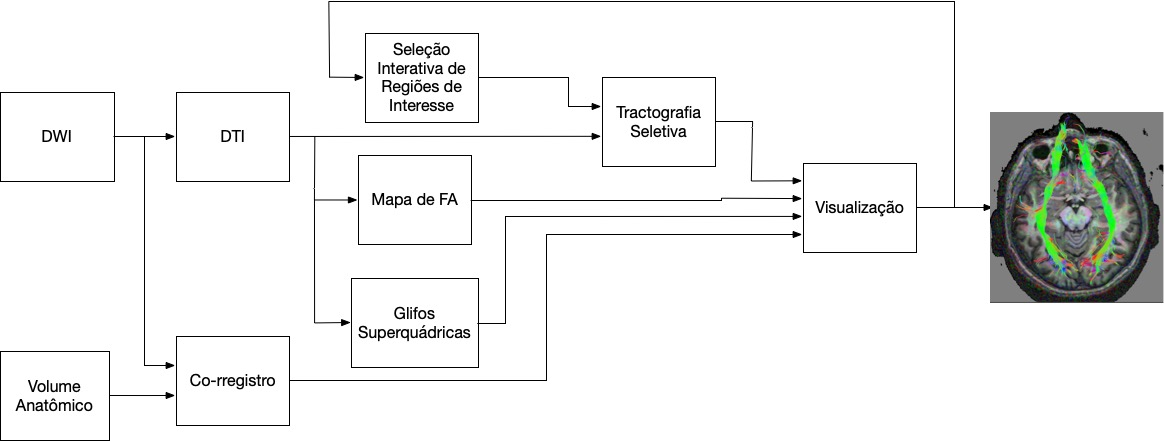
\includegraphics[width=1.0\linewidth, angle=0]{figs/Fluxogramas/PipelineDTI_tracto.jpg}
    \caption{Fluxograma para tractografia implementado no VMTK-Neuro.}
    \label{fig::PipelineDTI_tracto}
\end{figure}

Estas ferramentas consistem na visualização em tempo interativo de tensores de difusão mapeados em glifos superquádricos \cite{Kindlmann2004} renderizados sobre as suas respectivas amostras (figura \ref{fig::intro_ex_DTI_glifos}), tractografia (figura \ref{fig::intro_ex_DTI_tractografia}) e o corregistro de volumes de difusão com volumes anatômicos T1.

Na tractografia baseada em DTI, o VMTK-Neuro possui ferramentas de interatividade que possibilitam que o usuário possa inferir sobre as regiões do volume que contém os tratos a serem analisados, bem como filtrar fibras de interesse e eliminar fibras espúrias. Adicionalmente, parâmetros relacionados a reconstrução, que podem diferir de acordo com a região de análise do usuário, também são configuráveis. O algoritmo de tractografia apresenta resultados visuais em tempo interativo para as formas de interação mencionadas.




\section{Objetivos}
\label{sec::objetivos}

A contribuição esperada para o presente trabalho é a implementação e validação de um algoritmo de tractografia interativo baseada em um método de imageamento HARDI como um protótipo ao VMTK-Neuro. Para alcançar este objetivo, o trabalho está esquematizado no fluxograma da figura \ref{fig::flowchart_trabalho_intro}.

\begin{figure}[ht]
   \centering
       \addtolength{\leftskip} {-2cm} % increase (absolute) value if needed
    \addtolength{\rightskip}{-2cm}

    %\vspace*{3mm}
    \centering
    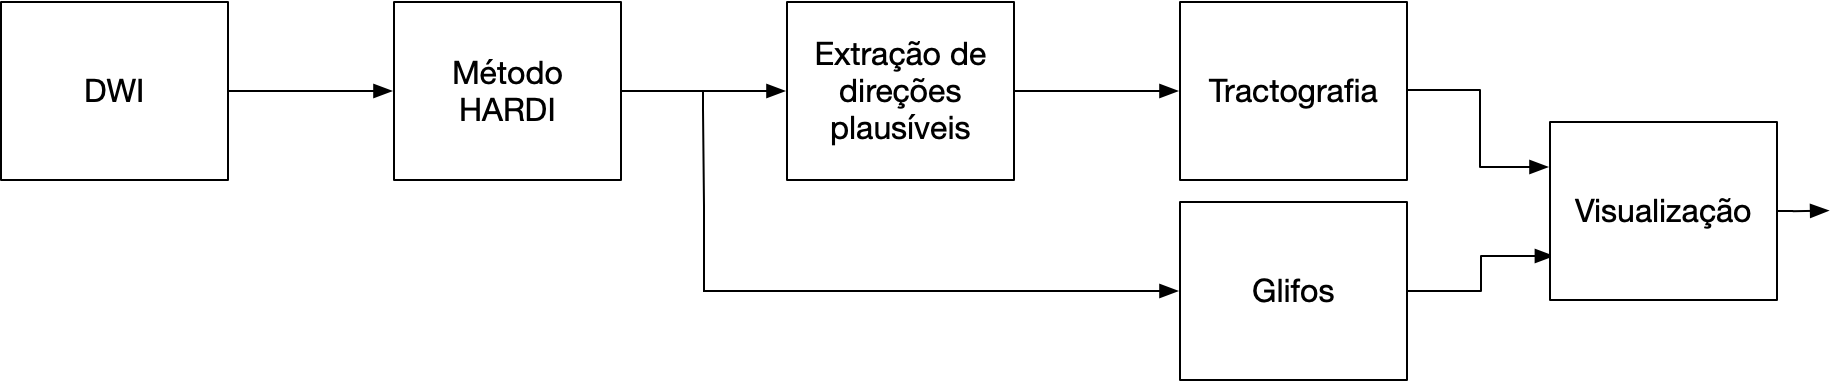
\includegraphics[width=.9\linewidth, angle=0]{figs/Fluxogramas/flowchart_trabalho_intro.png}
    \caption{Fluxograma de trabalho}
    \label{fig::flowchart_trabalho_intro}
\end{figure}

A partir do fluxograma, então, é necessário ter de forma esquemática a resposta a questões relativas a:

\begin{itemize}
\item escolha e implementação de um método de imageamento HARDI; \textcolor{red}{de alta resolução angular (HARDI)};
\item visualização interativa de perfis de difusão gerados através do método HARDI;
\item como extrair direções plausíveis de fibras a partir dos perfis de difusão e sua visualização e
\item como implementar um algoritmo de tractografia de forma interativa.
\end{itemize}


\textcolor{red}{A expectativa é aplicar os resultados na implementação do fluxograma mostrado na Figura ??? no VMTK-Neuro ...}



\todo[inline]{Sugiro que mostre em algum ponto uma visão geral do fluxo de controle da sua proposta de construção de tractografia a partir de DWIs de alta resolução angular.}

\section{Desafios}
\label{sec::desafios}

Para implementação do sistema, muito da infraestrutura necessária para alcançar os objetivos estabelecidos estão implementadas no VMTK-Neuro para visualização de volumes DWI por DTI. Portanto, muitos dos desafios enfrentados dizem respeito a questões de implementação do método HARDI, seu esquema de visualização em glifo e o algoritmo de tractografia associado.

A própria implementação matemática de um método HARDI para sintetizar o perfil de difusão é uma tarefa desafiadora. Os métodos demandam uma quantidade de memória razoavelmente maior que o DTI, que pode ser codificado na memória com apenas 6 elementos (matriz 3x3 simétrica). Métodos HARDI não estabelecem um critério mínimo, entretanto precisam de centenas de elementos para descreverem o perfil de difusão de forma razoável.

A implementação de um esquema de renderização de perfis de difusão em tempo interativo é algo desafiador pela grande quantidade de dados necessários para sintetizar um glifo. Além disso, na renderização tridimensional de volumes de difusão, este esquema de renderização é integrado ao próprio esquema de renderização do volume, bem como o sistema de detecção de amostras aparentes presente no \textit{software}, o que diminui a margem de tempo de execução do esquema.

O último desafio diz respeito à implementação de um algoritmo em tempo interativo de tractografia, que precisa ter seu cômputo rápido o suficiente para seguir as interações feitas pelo usuário.


\todo[inline]{Não acha que aqui você tem que focar nos desafios relacionados à interatividade, uma vez que o item 4 listado na seção anterior já se encontra implementado no VMTK. Só precisa de algumas adequações. Quais são os desafios para tornar um algoritmo de reconstrução de fibras a partir de HARDI (DWI de alta resolução angular) interativo? Quais restrições devem ser observadas?}

\sout{No que diz respeito à escolha do método HARDI utilizado, integramos a sua formulação matemática diretamente no VMTK-Neuro. Os principais critérios para sua escolha se devem a sua adequabilidade em tractografia, sua usabilidade em DWIs de baixa resolução angular e simplicidade.}

\sout{Pelo demanda de visualização interativa do VMTK-Neuro, objetivamos que a visualização dos perfis de difusão do método HARDI para os voxels visíveis na tela seja em tempo interativo. Assim, o usuário tem a informação em tempo real dos perfis de difusão nas regiões do volume a serem analisadas.}

\sout{Assim como a visualização dos perfis de difusão, também objetivamos a visualização interativa da tractografia. As vantagens desta abordagem consistem em dar ao usuário o poder de, através da visualização, escolher regiões de análise e setar os melhores parâmetros de acordo com o seu trato de interesse, indivíduo analisado e aquisição DWI.}

%\section{Contribuições}
%\label{sec::contribuicoes}
%
%
%Este trabalho apresenta duas contribuições:
%
%\begin{itemize}
%	\item proposição de um algoritmo para visualização em tempo %interativo de perfis de difusão para métodos HARDI e
%	\item proposição e validação de um algoritmo de tractografia %em tempo interativo baseado em informações direcionais de %fibras.
%\end{itemize}


%O trato corticoespinhal (CST) (Figura \ref{fig::CST_anatomia}) será o ponto de partida de análise e um ponto central para validação do algoritmo para o escopo deste trabalho de mestrado.

\section{Organização}
\label{sec:intro_organizacao}

Como penso em fazer:
Obs: Trabalhos relacionados integrados a cada capítulo.

1)Implementação do método HARDI e extração de fibras subjacentes através de picos.

2) Glifos;

3) Tractografia;

4) Conclusões

\textcolor{red}{
\chapter{Decisões Iniciais??? Ou Trabalhos Relacionados}
\label{chapter::decisoesiniciais}
}

\section{Métodos HARDI}

Houveram mais de cem artigos que propuseram métodos de imageamento para descrever o perfil de difusão entre 2000-2010 \cite{descoteaux2015} e evidentemente precisamos fazer uma seleção dos quais deles são mais relevantes para o nosso trabalho.

Os primeiros métodos HARDI propostos consistem no DSI \cite{wedeen2005} - proposto originalmente em 2000 - e presente na tese de doutorado de \citeonline{tuch2002}, juntamente com a abordagem multitensor e o QBI - este último que tem sido o mais popular e está também descrito em artigo \cite{TuchQBall2004}.

Há diferentes aplicativos livres que utilizam métodos HARDI para processamento de DWI, que estão ligados a grupos de pesquisa na área, nos quais restringimos o nosso horizonte a eles. Estes métodos são: GQI (DSI-Studio, !!refDSI), QBI (FSL, FiberNavigator), CSD (MRTrix, ExploreDTI).

Para implementação, o GQI foi escolhido para ser implementado neste trabalho, por suas seguintes características:

\begin{enumerate}
    \item Ser aplicável em categorias de aquisição com múltiplos valores $b$, o que não é presente no QBI;
    \item facilidade de implementação. O GQI não depende da codificação por harmônicas esféricas e interpolações no domínio esférico nas aquisições;
    \item boa aplicabilidade em volumes de mais baixa resolução angular \cite{yeh2010};
    \item ter parâmetros de regularização e filtragem integrados ao método.
\end{enumerate}

A grande desvantagem do GQI implementado na forma proposta por \citeonline{yeh2010} ocorre em questões computacionais. A codificação por amostras de funções esféricas requer uma quantidade maior de memória do que o armazenamento de dados como coeficientes de harmônicas esféricas, como é a abordagem da implementação do CSD e QBI nos softwares mencionados anteriormente.

%Alguns métodos HARDI nos quais há softwares associados a grupos de pesquisa na comunidade do DWI consistem no: GQI, implementado no DSI-Studio !!ref), QBI, implementado no FSL e o CSD, implementado no MRTrix
FiberNavigator????????!!



\todo[inline]{As decisões iniciais são tipicamente baseadas nos trabalhos relacionados. Portanto, sugiro que você apresenta as suas decisões iniciais contextualizadas no estado-da-arte.}

Baseado nos critérios apontados na seção \ref{sec::desafios}, neste capítulo descreveremos os critérios de escolha para o método HARDI utilizado no trabalho bem como a modalidade de tractografia escolhida.

\section{\sout{Escolha do método HARDI}Técnicas de Síntese de Direções de Difusão}

No que diz respeito a adequabilidade para tractografia, não há métodos que se sobressaem em relação a outros métodos nas mais diferentes condições experimentais \cite{SCHILLING2019194}.

\todo[inline]{Sugiro que façs aqui uma espécie de survey dos métodos ... Fica a seu critério a classificação ... pode ser por forma de amostragem como em \url{https://www.researchgate.net/publication/319558026_High_Angular_Resolution_Diffusion_Imaging_HARDI/link/59e88db8a6fdccfe7f8e8a4f/download} ... Sugiro que poderia fazer um merge com capítulo 3.}

\textcolor{red}{\subsection{Amostragem de Baixa Resolução (DTI)}} 

\textcolor{red}{\subsection{Amostragem de Alta Resolução (HARDI)}}

\todo[inline]{Amostragem Não-Uniforme -- Overplus, Amostragem Uniforme em Coordenadas Esféricas, Amostragem Uniforme em Coordenadas Cartesianas}


\textcolor{red}{\subsection{Análise Comparativa}}

\todo[inline]{DTI é a técnica mais clássica. Sugiro que faça um pequeno comentário da superioridade de HARDI em relação a DTI.}

\todo[inline]{Há uma mistura de conceito quando se trata de HARDI. Não ficou claro para mim o que você chama de HARDI.}

\todo{Acho que não tem muito sentido.}\sout{Não encontramos trabalhos que avaliem de forma sistemática diferentes métodos HARDI aplicados a volumes de baixa resolução angular.} \citeonline{daducci2014} faz um estudo comparativo entre \todo{Que métodos?}diferentes métodos HARDI, mas a aquisição é variável para os métodos utilizados. No desafio ISMRM 2015 \cite{TractometerTool}, que utiliza um volume artificial com resolução angular de 32 e valor $b = 1000s/mm^2$, não há uma conclusão sobre \todo{Qual método? Da aquisição até tractografia há diferentes passos e cada passo pode ser resolvido por diferentes métodos?} o melhor método HARDI a ser utilizado para tractografia.

O método DSI esteve fora de cogitação por possuir mais requerimentos na aquisição e ter uma reconstrução mais exigente computacionalmente que o QBI \cite{tournier2011}.

Tanto o GQI quanto a abordagem multi-tensor não possuem a mesma relevância nos mais diversos trabalhos quanto o QBI e o CSD. Acerca do GQI, \citeonline{yeh2010} mencionam a similaridade de resultados dos perfis de difusão com o QBI e sua vantagem no que diz respeito a ter incorporado no método de imageamento proposto modalidades de aquisição que não são englobadas pelo QBI, o que o torna atrativo em futuros trabalhos.

Entre o CSD e o QBI, escolhemos o QBI pela facilidade de implementação neste estágio inicial desta pesquisa. Vale salientar que implementamos o algoritmo proposto por \citeonline{TuchQBall2004} e que \citeonline{descoteaux2007_QBI} propuseram uma versão que provê o cômputo mais rápido do QBI utilizando as funções base harmônicas esféricas, que poderá ser implementado como evolução deste trabalho.

\textcolor{red}{\section{Renderização de ODFs}}

\textcolor{brown}{\citeonline{peeters2009} apresentou pela primeira vez um esquema de renderização para esta categoria de glifos, nos quais são aperfeiçoados por \citeonline{peeters2011} e \citeonline{hlawitschka2012}. Estes esquemas utilizam a abordagem \textit{raycasting}.}

\textcolor{brown}{No VMTK-Neuro, um dos algoritmos de renderização do tensor difusão por glifos superquádricos é feita por instanciações de uma malha esférica, no qual é customizada por parâmetros particulares a cada tensor de difusão referentes a cada \textit{voxel} detectado e posicionado na cena de acordo. Este esquema de renderização desenha os glifos em tempo interativo.}

\todo[inline]{Inclui a sua análise em frente dos resultados já existentes e como pretende aplicá-los.}

\textcolor{brown}{Pela maior simplicidade e boa efetividade da renderização por instanciações de uma malha esférica, o esquema desenvolvido neste trabalho utiliza esta abordagem.}

\textcolor{red}{\section{Extração de Direções Plausíveis de Fibras}}

!!(eu tenho que estudar um pouco disso pra entender o que foi feito)
Como pré-processamento, \citeonline{descoteaux2007}, inspirados por \citeonline{Tournier2004DirectEO}, sugerem uma transformação na ODF com o objetivo de aumentar a magnitude dos máximos em relação a partes suaves, utilizando a deconvolução esférica, o resultado da transformação é chamado de fODF.

\todo[inline]{Desloquei o texto abaixo para cá para mostrar os trablhos/discussões já existentes sobre este assunto ... Precisa ser organizado e adaptado para o seu contexto.}

\textcolor{brown}{
 O algoritmo, chamado de \todo{referência?}dODF-STR, gera um \textit{streamline}, cujo processo é feito na escolha de uma e somente uma direção baseado nos picos extraídos de uma ODF. Em comparação com a outra abordagem proposta, chamada de \todo{referência?}SPLIT-STR, gera bifurcação dos \textit{streamlines} para múltiplas direções extraídas do modelo.
}

\todo[inline]{Anderson \citeonline{Anderson2005} propôs FORECAST.}

\todo[inline]{Em \citeonline{Hess2006} ODFs são redefinidas em termos de harmônicos esféricos.}

\todo[inline]{\citeonline{descoteaux2007}: Um termo de regularização baseado no operador de Laplace-Beltrami na transformada Funk-Radon para aprimorar a acurácia na detecção dos máximos de ODF.}

\textcolor{brown}{
\citeonline{descoteaux2007} propõem um \todo{qual pré-processamento? }pré-processamento que consiste no afiamento da ODF, na qual visa prover um maior destaque aos picos e regiões de mais alta magnitude na ODF, conforme a figura \ref{fig::sharpening}. Com dados artificiais, o autor faz um experimento no qual a extração de direção de fibras é feito com a ODF de difusão extraída do QBI, a ODF após o processamento, a função de distribuição de orientação de fibra extraída do método deconvolução esférica filtrada para diferentes relações sinal ruído. O resultado do experimento atesta que a precisão da extração de picos aumenta com o pré-processamento, e tem um grau parecido com a abordagem de deconvolução esférica. Este pré-processamento não foi contemplado neste trabalho de mestrado.
}

\begin{figure}[h]
%\subfigcapskip = -5pt
    \centering
    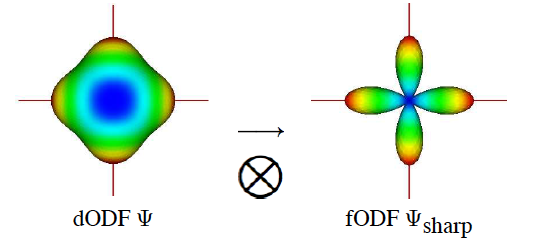
\includegraphics[width=.45\linewidth, angle=0]{figs/Tractografia/sharpening.png}
     \caption{Operação de afiamento de ODF. A função esférica a esquerda mostra um glifo de ODF obtida através de um sinal HARDI simulado e a direita a sua transformação em uma ODF afiada. \\
     Fonte: \cite{descoteaux2007}
     }
     \label{fig::sharpening}
 %   \hspace{1pt}
\end{figure}

\textcolor{brown}{
Evidentemente que não é possível fazer uma tractografia que computa tratos em tempo interativo com uma abordagem idêntica como \citeonline{descoteaux2007}, que a cada iteração interpola trilinearmente 1281 amostras de ODF para computar picos no processo de decisão da direção do passo da curva em um \textit{loop}.
}

\todo[inline]{Vale incluir \citeonline{Aganj2009}. Nele os autores explicam a causa da imprecisão no modelo de ODF, discutem a razão do pós-processamento de ``aguçamento'' das  ``plausíveis orientações'' e propõem uma reformulação.}

\todo[inline]{Fibernavigator: não entendi o que você escreveu. Em \citeonline{Chamberland2016} não há nenhuma proposta nova em relação à detecção de picos mais relevantes. Os autores aplicaram as técnicas já propostas.}

\textcolor{brown}{
A estratégia adotada então para este impasse é similar ao proposto por \citeonline{Chamberland2016}, que consiste em computar informações de direções de fibras na sua totalidade antes da execução da tractografia. Estes dados são acessados na tractografia e nas regiões \textit{intra-voxel}, a estimativa das direções é feita através da interpolação pelo vizinho mais próximo.
}

\textcolor{brown}{
Para atenuar o erro gerado pela atribuição do vizinho mais próximo, adotamos uma estratégia de aumentar as amostras de ODF para extração de informações direcionais neste respeito utilizando interpolação trilinear. Os resultados apresentados !!(na seção???) utilizam picos de um volume com a resolução duplicada nas direções x, y, z (de 2x2x2 $mm^3$ para 1x1x1 $mm^3$).
}

\textcolor{brown}{
Uma questão pertinente acerca do aumento de amostras é se ela deve ser feita no DWI, no qual o método de difusão é aplicado sobre o volume super amostrado ou se pode ser feito diretamente nos valores de ODF. A literatura não é clara neste aspecto. !!Referencias!
}


\section{Tractografia}
\label{sec::decisoesiniciais_tractografia}

A tractografia consiste em traçar fibras no cérebro por meio de modelos matemáticos a partir um volume de difusão. Há dois tipos de abordagem, que consistem nos determinísticos e probabilísticos.

A tractografia determinística consiste na integração de linhas representativas de fibras do cérebro. Estas linhas são estimadas em um processo iterativo, no qual é iniciado em um conjunto de pontos (sementes), e o passo de cada iteração é obtido através de informações direcionais provenientes de um método de \sout{difusão}\textcolor{red}{estimativa das direções de difusão locais a partir de volumes DWI}. \sout{O processo iterativo é terminado por meio de um critério apropriado}\textcolor{red}{O critério de parada do processo iterativo pode variar entre as implementações.} \cite{tournier2011}.


%A tractografia determinística se baseia em um processo iterativo que consiste em, tendo em posse um conjunto de pontos nos quais o algoritmo é iniciado (sementes), há uma integração de linhas cujas direções são estimadas através de informações direcionais de um método de imageamento de difusão. Estas linhas são representativas da fibra estimada. O processo iterativo é terminado por meio de um critério apropriado \cite{tournier2011}.

A tractografia probabilística consiste na consideração do comportamento de difusão de forma aleatória em cada ponto no volume, e gera como resultado um mapa de probabilidade de tratos entre um conjunto de pontos de partida e chegada \cite{DTI_Handbook}. A partir do mapa, pode-se inferir sobre a probabilidade com que uma determinada conexão pode ocorrer \cite{tournier2011}. %\citeonline{hagman2003} propôs um método probabilístico utilizando o tensor de difusão

No que diz respeito a comparações da natureza entre as duas abordagens, as probabilísticas não possuem a restrição de ter um trato por semente e, dado dois pontos de escolha no cérebro de forma aleatória, esta abordagem irá encontrar caminhos entre ambos, nos quais cada um está associado a uma métrica de conectividade. Neste sentido, a abordagem probabilística é mais flexível que a determinística, entretanto o resultado gerado não deve ser interpretado como a conectividade anatômica \cite{tournier2011}. 

Por outro lado, as abordagens determinísticas geram resultados que permitem uma correlação com a conectividade anatômica e são utilizadas para estudo de tratos conhecidos que tem um conjunto de sementes estabelecidas e protocoladas \cite{tournier2011}. Adicionalmente, as abordagens determinísticas geralmente são menos custosas computacionalmente \cite{DTI_Handbook}.

A tractografia determinística foi escolhida neste trabalho por ser menos demandante computacionalmente e pela maior correlação com a conectividade de fibras do cérebro imageado através do DWI e que tem uma maior aplicabilidade para planejamento cirúrgico.

\textcolor{red}{
\chapter{Trabalhos Relacionados??? Ou Materiais e Métodos??}
\label{cap:metodos}
}

\todo[inline]{Seções 3.3, 3.4, 3.5, 3.2.1, 3.2.2, 3.2.3 e 3.2.4 não poderiam estar integradas de forma mais geral no Capítulo 2 como ferramentas encontradas na literatura. Não são específicas do VMTK. Sugiro que neste capítulo só faz referência às técnicas implementadas no VMTK.}

Nesta capítulo são apresentados os trabalhos relacionados as decisões iniciais tomadas, bem como funcionalidades correlatas integradas ao VMTK-Neuro.

\textcolor{red}{
\section{Dados}
}

\section{VMTK-Neuro}
\label{AlgoritmosVMTK}


No VMTK-Neuro, há a implementação de ferramentas de processamento e visualização para volumes de difusão e que estão diretamente relacionadas ao presente trabalho. Estas ferramentas, que usam como base o DTI, estão esquematizadas no fluxograma da figura \ref{fig::PipelineDTI_tracto}.

%ORIGINAL -> FLUXOGRAMA VMTK NEURO
%\begin{figure}[ht]
%   \centering
%       \addtolength{\leftskip} {-2cm} % increase %(absolute) value if needed
%    \addtolength{\rightskip}{-2cm}
%
%    %\vspace*{3mm}
%    \centering
%    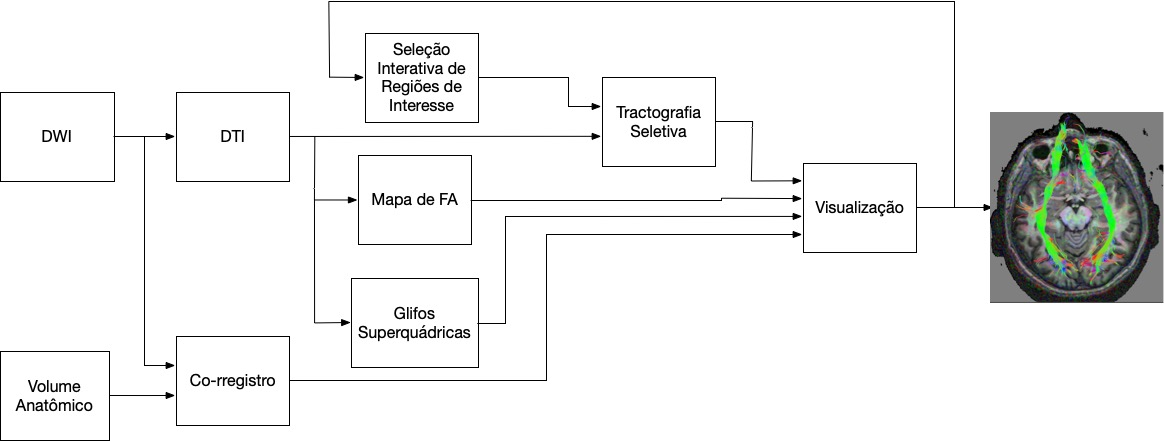
\includegraphics[width=1.0\linewidth, %angle=0]{figs/Fluxogramas/PipelineDTI_tracto.jpg}
%    \caption{Fluxograma para tractografia implementado %no VMTK-Neuro.}
%    \label{fig::PipelineDTI_tracto}
%\end{figure}

\pagebreak
\subsection{DTI}
O DTI é um método de imageamento para difusão que consiste no mapeamento de um conjunto de valores de coeficientes aparentes de difusão (ADC - \textit{apparent diffusion coefficient}) em um ponto $(x, y, z)$ no DWI em um modelo gaussiano para difusão. 

A quantificação da difusão a partir do sinal adquirido se dá através da equação de Stejskal-Tanner (equação \ref{eq::Stejskal}) \cite{DTI_Handbook}.

\begin{equation}
    S = S_0 e^{-bD},
    \label{eq::Stejskal}
\end{equation}

onde $D$ representa o valor de difusão, $S$ é o valor do sinal de difusão, $S_0$ é o sinal de difusão no volume $b_0$ e $b$ é um valor constante, que é função dos parâmetros de aquisição. A equação \ref{eq::adc} explicita o valor de difusão na equação a partir da equação \ref{eq::Stejskal}.

\begin{equation}
\label{eq::adc}
    D = \frac{-ln(\frac{S}{S_0})}{b}
\end{equation}

A regressão ao modelo gaussiano é feita a partir das direções amostradas dos gradientes de ponderação por difusão associadas ao seus respectivos valores ADC, com média zero. O tensor de difusão, representado na equação \ref{eq::tensor}, é proporcional à matriz de covariância obtida na regressão.

\begin{equation}
\label{eq::tensor}
\mathbf{D} = 
\begin{bmatrix}
D_{xx} & D_{xy} & D_{xz} \\ 
D_{xy} & D_{yy} & D_{yz} \\ 
D_{xz} & D_{yz} & D_{zz}  
\end{bmatrix}
\end{equation}


Os valores obtidos na decomposição em autovalores do tensor de difusão (equações \ref{eq::decomposicao1}, \ref{eq::decomposicao2} e \ref{eq::decomposicao3}) tem aplicações importantes no entendimento do comportamento da difusão através do modelo DTI. Os autovetores $\mathbf{e}_1$, $\mathbf{e}_2$ e $\mathbf{e}_3$ do tensor de difusão representam três direções ortogonais, cujos seus respectivos autovalores $\lambda_1$, $\lambda_2$ e $\lambda_3$ representam suas respectivas magnitudes de difusão, que são máximos. 
\begin{equation}
\label{eq::decomposicao1}
\mathbf{D} = \mathbf{E}*\mathbf{\Lambda}*\mathbf{E}^{-1}
\end{equation}
onde
\begin{equation}
\label{eq::decomposicao2}
\mathbf{\Lambda} = \begin{bmatrix} 
\lambda_1 & 0 & 0 \\ 
0 & \lambda_2 & 0 \\ 
0 & 0 & \lambda_3  
\end{bmatrix};
\lambda_1 > \lambda_2 > \lambda_3
\end{equation}

\begin{equation}
\label{eq::decomposicao3}
\mathbf{E} = 
\begin{bmatrix} 
e_{1x} & e_{2x} & e_{3x} \\ 
e_{1y} & e_{2y} & e_{3y} \\ 
e_{1z} & e_{2y} & e_{3z}  
\end{bmatrix};
\mathbf{|e_1|} = \mathbf{|e_2|} = \mathbf{|e_3|} = 1
\end{equation}

O tensor de difusão e seus respectivos autovalores e autovetores são utilizados como base para cômputo de glifos superquádricos, tractografia e mapa de anisotropia fracionada (\textit{fractional anisotropy} - FA) codificada por cores. que estão descritos de forma detalhada mais adiante.

Neste trabalho, chamaremos as direções associadas ao maior e segundo maior autovalores de difusão $\mathbf{e}_1$ e $\mathbf{e}_2$ de direção principal de difusão e direção secundária, respectivamente.

\subsection{Mapa FA codificado por cores e corregistro com dados neuroanatômicos.}



O mapa FA codificado por cores exibe informações espaciais referente a direções dominante de difusão, bem como o grau de anisotropia do processo de difusão.
A relação entre anisotropia fracionada e os autovalores do tensor de difusão é dada através da equação \ref{eq::fa}, onde $\overline{\lambda}$ é a média dos três autovalores. O FA tem valor máximo 1 para uma difusão que ocorre em somente uma direção e mínimo 0 para o caso isotrópico.

\begin{equation}
\label{eq::fa}
    FA = \sqrt{\frac{3}{2}}.\sqrt{\frac{(\lambda_1 - \overline{\lambda})^2 + (\lambda_2 - \overline{\lambda})^2 + (\lambda_3 - \overline{\lambda})^2}{\lambda_1^2 + \lambda_2^2 + \lambda_3^2}}
\end{equation}


O mapa consiste em um volume, cujas cores são definidas são definidas \textit{voxel} a \textit{voxel} em função do FA e o autovetor associado a maior difusão $\mathbf{e}_1$ através da equação \ref{eq::FAMap}.

\begin{equation}
\label{eq::FAMap}
    (r,g,b) = FA*(|e_{1x}|,|e_{1y}|,|e_{1z}|)
\end{equation}

A figura \ref{fig::MapaFA} ilustra um mapa FA codificado por cores e é perceptível que nesta forma de visualização não se distingue a anatomia geral do cérebro. Para sanar este problema, é integrada no VMTK a funcionalidade do corregistro do mapa com um volume de ressonância magnética ponderada em T1, como mostrado na figura \ref{corregistroFAT1}.

\begin{figure}[H]

%\subfigcapskip = -5pt
    \centering

    %\vspace*{3mm}
    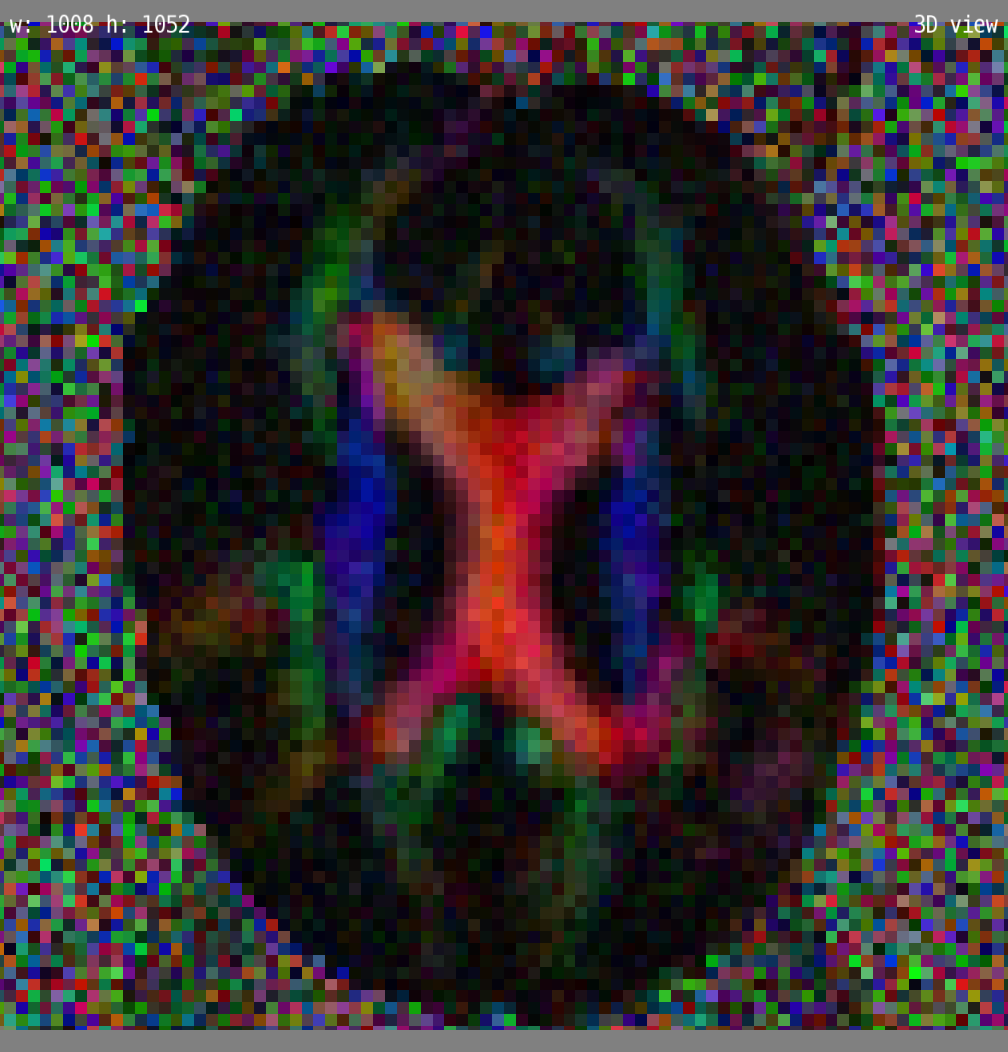
\includegraphics[width=0.45\linewidth, angle=0]{figs/Exemplo_Trabalhos_Relacionados/MapaFA.png}
    \caption{Fatia axial de um mapa FA codificado por cor. As cores representam a direção de difusão máxima; vermelho = esquerda-direita, azul = cranio-caudal, e verde = anterior-posterior}
    %\legend{Fonte: VMTK-Neuro}
    \label{fig::MapaFA}
 %   \hspace{1pt}
\end{figure}

O corregistro faz o alinhamento entre um volume de difusão/mapa FA com um volume anatômico T1. Adicionalmente, o aplicativo VMTK-Neuro oferece a possibilidade de visualizá-los sobrepostos, em que a ponderação na opacidade de cada um dos volumes na visualização é ajustável pelo usuário.

\begin{figure}[H]
\centering
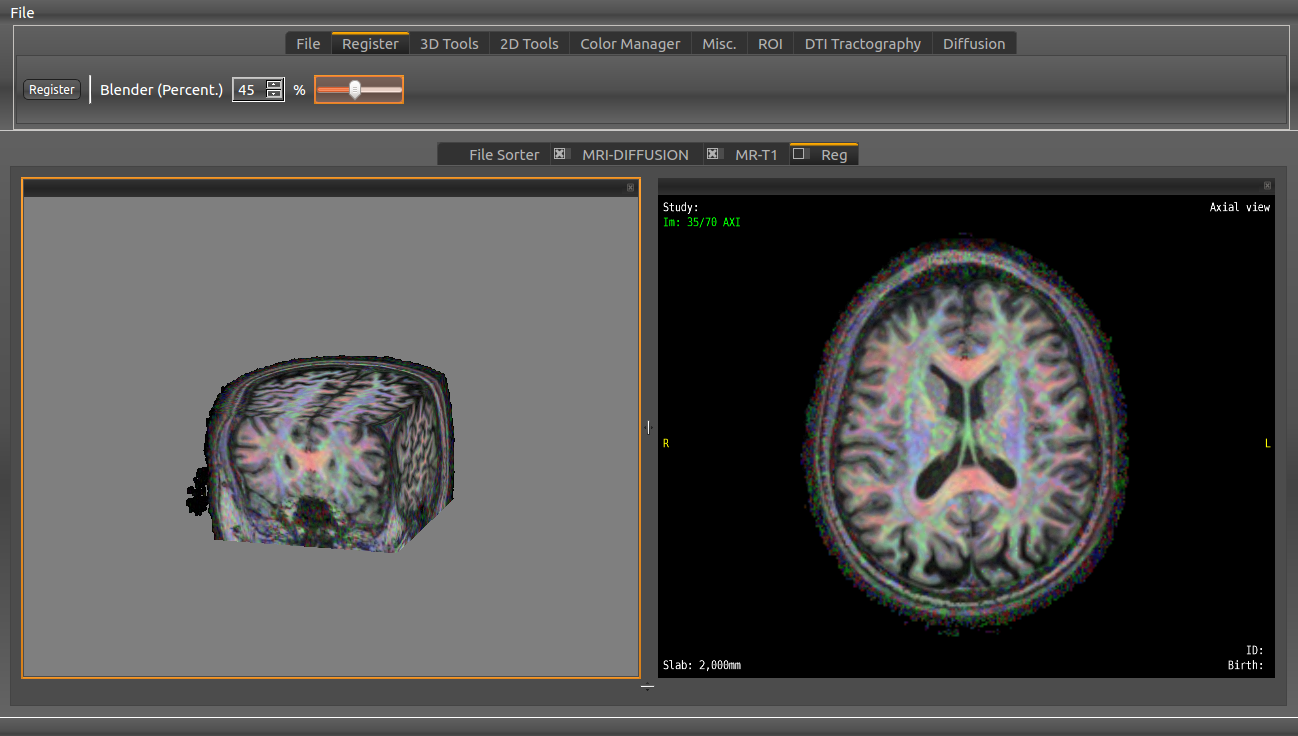
\includegraphics[scale = 0.3]{figs/Exemplo_Trabalhos_Relacionados/corregistro.png}
\caption{Interface do VMTK-Neuro para visualização do volume anatômico e do mapa FA codificado em cores corregistrados.}
\label{corregistroFAT1}
\end{figure}

\subsection{Tensor de difusão por glifos superquádricos}
\label{ssec::supequadricos}

É integrado ao VMTK-Neuro um esquema de visualização de tensores de difusão através de glifos superquádricos \cite{Kindlmann2004}, conforme mostrado na figura \ref{fig::intro_ex_DTI_Superquadrica}. Os glifos são renderizados em tempo interativo nos seus respectivos \textit{voxels}, tanto em fatias do volume, quanto na sua renderização tridimensional.

Na visualização de fatias, a inferência dos \textit{pixels} aparentes na tela consistem na leitura do índice da fatia mostrada, no qual os glifos são posicionados no ponto central do seu respectivo \textit{pixel}.

Na renderização tridimensional, há uma funcionalidade para detecção de \textit{voxels}, em que cada um possui uma matriz de translação para o seu respectivo centro na cena. A detecção é baseada em \textit{raycasting} computado sobre o volume na GPU, que foi proposto e implementado por \citeonline{raphael_dissertacao}.



O objetivo do glifo é a disponibilidade de mais uma ferramenta de visualização para o comportamento de difusão \textit{voxel} a \textit{voxel}, o que pode ser utilizado pelo usuário no suporte à escolha de regiões de sementes para iniciar as integrações lineares em tractografia e averiguar visualmente a qualidade de aquisição das amostras dos sinais de difusão.


\subsection{Tractografia baseada em DTI e seletividade}
\label{ssec::tractografia_e_seletividade}


%!!Diferenciar tractografia determinística e probabilistica.
%Pode-se ainda categorizar a tractografia quanto a abordagem do método, que são as abordagens determinísticas e probabilísticas.



A tractografia presente no VMTK-Neuro foi baseado no nos métodos determinísticos baseados em DTI propostos por \citeonline{Weinstein1999} e \citeonline{basser2000}. As demandas que motivaram escolha do método vem do baixo custo computacional do modelo e a possibilidade de renderização de linhas representativas das fibras do cérebro de forma interativa, imediatamente após a seleção das sementes.


%Os métodos consistem na seleção de um conjunto de sementes pelo usuário e a partir delas, há a integração iterativa de linhas até que um critério de parada seja satisfeito.

No processo iterativo, a direção da integração de linhas é feita levando em consideração a direção da integração anterior e um conjunto de grandezas associadas ao tensor de difusão no ponto atual \cite{Weinstein1999}.


É definido três coeficientes de anisotropia para categorização dos \textit{voxels} de acordo com os autovalores do tensor de difusão $\lambda_1, \lambda_2$ e $\lambda_3$ ($\lambda_1 \geq \lambda_2 \geq \lambda_3$) , chamados de anisotropia linear ($c_l$), planar ($c_p$) e esférica ($c_s$). As expressões que relacionam as anisotropias e os autovalores do tensor estão representadas nas equações \ref{eq::cl}, \ref{eq::cp} e \ref{eq::cs}.

\begin{equation}
\label{eq::cl}
    c_l = \frac{\lambda_1 - \lambda_2}{\lambda_1 + \lambda_2 + \lambda_3}
\end{equation}

\begin{equation}
\label{eq::cp}
    c_p = \frac{2(\lambda_2 - \lambda_3)}{\lambda_1 + \lambda_2 + \lambda_3}
\end{equation}

\begin{equation}
\label{eq::cs}
    c_s = \frac{3\lambda_3}{\lambda_1 + \lambda_2 + \lambda_3}
\end{equation}

\citeonline{Weinstein1999} definem os vetores de advecção, $\mathbf{v}_{in}$ e $\mathbf{v}_{out}$, que tem como função a estabilização do processo de \textit{tracking} das linhas. O vetor $\mathbf{v}_{in}$ é direção de propagação da iteração anterior e $\mathbf{v}_{out}$  consiste na direção de entrada da tractografia transformada pelo tensor de difusão ($\mathbf{v}_{out} = \mathbf{D}\mathbf{v}_{in}$).

A partir das métricas de anisotropia e dos vetores de advecção, \citeonline{Weinstein1999} definem condições desejáveis para integração de linhas na tractografia baseadas na categoria de anisotropia no ponto em análise, que estão presentes na tabela \ref{tab::tracto_desirable_conditions}. A equação \ref{eq::tractografia_weinstein} é sugerida pelos autores por satisfazer estas condições. Na equação, $\textbf{v}_{prop}$ consiste no passo de propagação e $w_{punct}$ é um parâmetro contido no intervalo [0,1] controlado pelo usuário que está relacionado à decisão do algoritmo acerca do  para o passo de propagação no caso de anisotropia planar e esférica.

\begin{table}[h]
\centering
\begin{tabular}{|c|c|c|}
\hline
\textbf{Anisotropia} & \textbf{Direção de propagação anterior} & \textbf{Saída desejada} \\ \hline
Linear               & Qualquer                                & $\mathbf{e}_1$                   \\ \hline
Planar               & Tangencial ao plano                     & $\mathbf{v}_{in}$ ou $\mathbf{v}_{out}$   \\ \hline
Planar               & Normal ao plano                         & $\mathbf{v}_{out}$            \\ \hline
Esférica             & Qualquer                                & $\mathbf{v}_{in}$ ou $\mathbf{v}_{out}$   \\ \hline
\end{tabular}
\caption{Condições desejáveis para decisões para o passo na integração de linhas em tractografia \cite{Weinstein1999}}.
\label{tab::tracto_desirable_conditions}
\end{table}

\begin{equation}
\label{eq::tractografia_weinstein}
    \textbf{v}_{prop} = c_l\mathbf{e}_1 + (1 - c_l)(w_{punct}\mathbf{v}_{out} + (1-w_{punct})\mathbf{v}_{in})
\end{equation}


No aplicativo, o tempo entre a seleção de sementes e a renderização de linhas representativas dos tratos é interativo. Para este fim, o algoritmo de integração de linhas foi implementado na GPU utilizando a API OpenGL, em que o seu cômputo para cada um dos sentidos de cada semente é feito de forma paralela. O seu cômputo ocorre no compute shader, para versão do OpenGL iguais ou superiores a 4.2, ou no geometry shader, para versões inferiores.

Na implementação, em pontos localizadas entre voxels, é utilizado a interpolação trilinear para estimar cada um dos coeficientes do tensor de difusão.

Há três critérios de parada no processo de integração de linhas \cite{basser2000}. O primeiro se dá quando \textit{voxel} atual no processo iterativo apresenta uma anisotropia baixa, o segundo se refere a uma ângulo alto entre a direção do \textit{voxel} atual em comparação ao da iteração anterior e o terceiro diz respeito à chegada à superfície do volume.

A interatividade com o usuário se dá na construção das regiões de interesse (ROI - \textit{region of interest}), bem como parâmetros associados à tractografia. As sementes são um subconjunto das ROIs que apresentam um FA acima de um limiar. Os parâmetros associados a parada da tractografia (ângulo de interrupção, limiar inferior de anisotropia), FA mínimo para semente e o parâmetro $w_{punct}$ são ajustáveis pelo usuário.


Há também no VMTK-Neuro a funcionalidade de tractografia seletiva, que dá ao usuário a possibilidade de remoção de fibras reconstruídas em regiões irrelevantes ou indesejadas através dos filtros do tipo NOT, AND e de reconstrução por parte. O filtro NOT consiste na escolha de uma região para que seja excluída na reconstrução do trato em questão e a do tipo AND restringe as linhas para apenas as que passam pela região escolhida. A implementação foi  baseada nas funcionalidades do aplicativo Explore DTI \cite{exploredti2009}. A reconstrução por parte consiste em setar, com base na análise visual das outras direções principais por meio de glifos, mais de uma região de sementes ao longo de uma fibra.

\section{\textit{Q-Ball}}

Proposto por \citeonline{TuchQBall2004}, o QBI é um método de imageamento para difusão em que estima uma função de distribuição de orientação (\textit{orientation distribution function} - ODF) $\psi(\mathbf{u})$ em um ponto a partir de seus respectivo conjunto de amostras de sinal de difusão no DWI.

A implementação do QBI consiste na escolha de um domínio com $n$ direções de difusão de interesse, dadas por $\{\textbf{u} \}= \{ \textbf{u}_1, \textbf{u}_2, \textbf{u}_3 ... \textbf{u}_n\}$ em que queremos reconstruir um vetor ODF, dado por $ \boldsymbol{\psi} = \{ \psi(\mathbf{u}_1), \psi(\mathbf{u}_2), \psi(\mathbf{u}_3) ... \psi(\mathbf{u}_n)\}$, para cada ponto de interesse em um volume DWI, cujo conjunto de sinais de difusão associado é representado por $\boldsymbol{e} = \{ E(\mathbf{q}_1), E(\mathbf{q}_2), E(\mathbf{q}_3) ... E(\mathbf{q}_m)\}$ adquiridos sob o conjunto de gradientes $\{\textbf{Q} \}= \{ \textbf{q}_1, \textbf{q}_2, \textbf{q}_3 ... \textbf{q}_m\}$. 


A associação entre os sinais se dá através da transformada Funk-Radon (\textit{Funk-Radon Transform} - FRT) aplicada em $ \boldsymbol{e}$. A FRT consiste no mapeamento entre funções esféricas, em que, para uma função $f(\mathbf{x})$, contínua, onde \textbf{x} é um vetor unitário, a sua FRT Ff(\textbf{x}) é dada por:

\begin{equation}
    \text{Ff}(\textbf{x}) = \int_{\textbf{u}\in C(\textbf{x})}f(\textbf{u})ds(\textbf{u})
\end{equation}
onde $C(\textbf{x}) = \{ \mathbf{u} \in  \mathbf{R}^3:|\mathbf{u}|=1 \text{ e } \mathbf{u}.\mathbf{x} = 0  \}$. C(\textbf{x}) é denominado equador de \textbf{x}, visto que o conjunto define direções contidas em um circunferência unitária ortogonal a \textbf{x}.


A figura \ref{fig::Esquema_QBall} ilustra, passo a passo, a obtenção da ODF extraída dos sinais de difusão.


\begin{figure}[H]

%\subfigcapskip = -5pt
    \centering

    %\vspace*{1mm}
    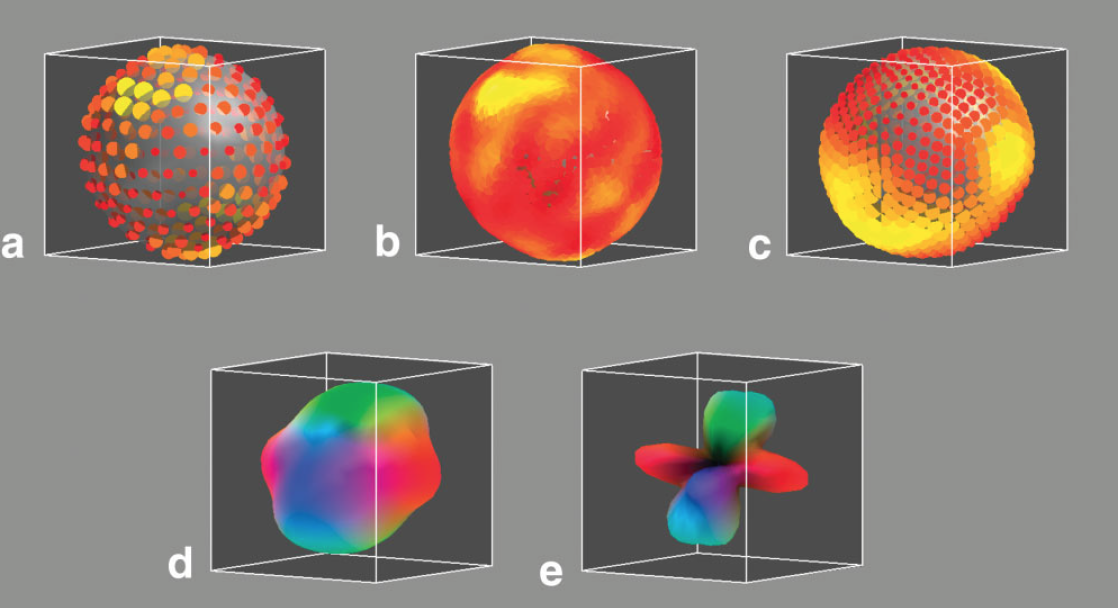
\includegraphics[width=0.9\linewidth, angle=0]{figs/Exemplo_Trabalhos_Relacionados/Esquema_QBall.png}
    \legend{\textbf{(a)} Sinal de difusão discretizado nos vértices de icosaedro tesselado. A intensidade do sinal é indicado por tamanho e cor (branco > amarelo > vermelho) dos pontos na esfera.   \textbf{(b)} Sinal interpolado para o conjunto de equadores.    \textbf{(c)} ODF de difusão calculado utilizando a FRT.   \textbf{(d)} Representação polar esférica da ODF.
    \textbf{(e)} ODF normalizada linearmente para o intervalo [0, 1]. \hspace{\textwidth}    Fonte: \cite{TuchQBall2004}}
    \caption{Reconstrução de ODF de difusão a partir do sinal de DWI através da FRT.}
    \label{fig::Esquema_QBall}
 %   \hspace{1pt}
\end{figure}

\section{Visualização de funções de distribuição de orientação}
\label{sec::trabalhos_relacionados_glifos}

O uso de glifos na forma de representação gráfica polar esférica é sugerida por \citeonline{TuchQBall2004} para representar o conjunto de dados relacionados a amostras de dODF. A sua representação consiste na modulação de uma malha esférica, na qual tem o seu raio $R(\textbf{u})$ escalonado por uma versão normalizada do valor da ODF na direção $\textbf{u}$. Uma forma de representação é dada pela equação \ref{eq::normglifo} e é mostrada na figura \ref{fig::Esquema_QBall}.e.

\begin{equation}
\label{eq::normglifo}
    R(\mathbf{u}) = \frac{\psi(\mathbf{u}) - min(\psi(\mathbf{u}))}{max(\psi(\mathbf{u})) - min(\psi(\mathbf{u}))}
\end{equation}

Estes itens geométricos dão uma noção de como é \todo{Não soa estranho?}\textcolor{brown}{o comportamento da difusão em um DWI}, inclusive em cruzamento de fibras. Regiões onde há um maior alongamento do glifo, representam áreas onde há uma maior difusão e uma maior chance de estarem alinhados com uma fibra.

Esta classe de glifos são amplamente utilizados como uma ferramenta de visualização para prova de conceito em trabalhos na área de DWI. Além de \citeonline{TuchQBall2004}, alguns trabalhos relacionados \todo{Só os utilizam? Não há trabalhos que procuram melhorar a sua renderização/visualização?}que os utilizam são: \citeonline{SCHILLING2019194}, para ilustrar a eficácia de métodos HARDI na detecção de direções de difusão, \citeonline{descoteaux2007}, para ilustrar o efeito de um\sout{a técnica} \todo{qual pré-processamento?}pré-processamento \sout{proposto} em ODFs que melhora a tractografia e \citeonline{yeh2010} os utilizam como ferramenta de visualização para o método de imageamento proposto em seu trabalho.


\section{\textit{Q-Ball} para tractografia}
\label{QBall_para_tractografia}

\citeonline{descoteaux2007} propõem técnicas de tractografia, ambas probabilísticas e determinísticas, utilizando o \textit{QBall} como uma generalização do que já fora proposto utilizando DTI.

!!No escopo deste trabalho, será considerado a tractografia determinística, que assim como o DTI, os tratos são estimados a partir da informação extraída das ODFs são relativas a direções e uma métrica de anisotropia.

\sout{!!(eu tenho que estudar um pouco disso pra entender o que foi feito)
Como pré-processamento, \citeonline{descoteaux2007}, inspirados por \citeonline{Tournier2004DirectEO}, sugerem uma transformação na ODF com o objetivo de aumentar a magnitude dos máximos em relação a partes suaves, utilizando a deconvolução esférica, o resultado da transformação é chamado de fODF.}

A abordagem determinística é uma extensão da técnica baseadas na integração de linhas na direção principal do tensor de difusão, no qual uma linha é integrada levando em consideração informações direcionais contidas em cada ponto no espaço até um critério de parada ser satisfeito.

No que diz respeito à extração das informações direcionais, \citeonline{descoteaux2007} sugerem que sejam extraídas direções referentes a máximos locais das funções esféricas. Evidentemente que, para evitar picos espúrios, é sugerido o uso de um limiar, abaixo do qual os máximos locais sejam removidos.

Os critérios de parada consistem nos mesmos que para o DTI: o critério angular, relativo a um alto ângulo entre as direções selecionadas entre a iteração atual e anterior, e o critério relativo a uma baixa anisotropia, que para a ODFs se chama anisotropia fracionada generalizada (\textit{generalized fractional anisotropy} - GFA), que é dado em função de amostras de ODF através da equação \ref{eq::gfa}:

\begin{equation}
\label{eq::gfa}
    GFA = \sqrt[]{\frac{n\sum_{i=1}^{n} (\psi(\textbf{u}_i) - \bar{\psi})^2}{(n-1)\sum_{i=1}^{n} \psi(\textbf{u}_i)^2}} ,
\end{equation}

onde $\psi(\textbf{u})$ é o valor de difusão para uma direção \textbf{u}, $n$ é a quantidade de direções no domínio e  $\bar{\psi}$ é o valor médio dos valores $\psi(\textbf{u})$, para todo domínio \textbf{u}. \citeonline{corbo2013} mencionam que há uma correlação linear entre a métrica de FA do DTI e GFA.

%\textcolor{brown}{A abordagem para estimar as ODFs no espaço intra-voxel consiste em estimar cada uma das amostras de ODF utilizando interpolação trilinear.}\todo{Não entendi ...}



%\chapter{Proposta}
%\label{proposta}


%O fluxograma do trabalho proposto, e que %está sendo implementado, consta na figura %\ref{fig::PipelineQBall_tracto}.
%!!!!
%\begin{figure}[H]
%
%%\subfigcapskip = -5pt
%    \centering
%   
%    \vspace*{1mm}
%    \includegraphics[width=0.9\linewidth, %angle=0]{figs/Fluxogramas/flowchart_t%rabalhocompleto.png}
%     \caption{Proposta.}
%    \label{fig::PipelineQBall_tracto}
% %   \hspace{1pt}
%\end{figure}
%
%O objetivo do projeto é a implementação %de um algoritmo de tractografia baseado %em ODFs no VMTK-Neuro com uma interface %interativa para o usuário. Para este fim, %o \textit{Q-Ball} é implementado para %modelar a difusão em ODFs, que tem seus %picos extraídos para se tornar a base do %processo de escolha na integração de %direções no algoritmo de tractografia.
%
%Interações com o usuário consistirão na %escolha de sementes para os tratos, bem %como a função de seletividade e a seleção %de parâmetros para os critérios de %parada.
%
%Vale destacar que a renderização de ODFs %em glifos por si só tem a função de ser %uma ferramenta para prova de conceito das %ODFs computadas e ajudar o usuário a ter %uma melhor visão da distribuição de %difusão \textit{voxel} a \textit{voxel}, %o que é altamente desejável. 
%
%
%
%Para alcançar o objetivo proposto no %trabalho, as seguintes tarefas foram %esquematizadas:
%
%\begin{enumerate}
%    \item \label{item:estudoconceito} %Estudo e entendimento dos desafios na %área de ressonância magnética de %difusão e tractografia.
%    \item \label{item:estudocodigo} %Estudo e entendimento do código do %VMTK-Neuro, em especial as %implementações relacionadas a %processamento de volumes DWI.
%    \item \label{item:qball} %Implementação do algoritmo %\textit{QBall} para estimativa de %ODFs.
%    \item \label{item:qballvisualização} %Mapeamento da ODF em glifos e sua %renderização em tempo real.
%    \item \label{item:qballprocessamento1%} Implementação de processamento para %extração de direções de difusão %plausíveis a partir das ODFs para %tractografia.
%    \item \label{item:tractografia1} %Desenvolvimento do algoritmo %tractografia.
%    \item \label{item:analise1} Avaliação %e análise dos tratos obtidos com essa %abordagem, usando como prova de %conceito as fibras neurais na %vizinhança do trato corticoespinhal.
%\end{enumerate}
%
%
%\chapter{Materiais e métodos}
%%\label{ssec:material}
%
%Para avaliação e validação das %atividades, serão utilizados dados %sintéticos fornecidos pelo desafio ISMRM %2015 (\textit{International Society for %Magnetic Resonance in Medicine}) %\cite{TractometerTool}.
%
%A motivação da proposição do desafio %ISMRM 2015 veio da falta de métodos %quantitativos para avaliar e comparar %diferentes algoritmos de tractografia. O %volume artificial gerado para a %competição simula realisticamente uma %ressonância magnética de difusão de um %cérebro, tendo os tratos possuindo um %padrão ouro e uma metodologia de %avaliação acessível, disponibilizada na %ferramenta \textit{Tractometer Scoring %Tool} . 
%
%As métricas utilizadas para avaliação são %o \textit{Overlap} (OL) e %\textit{Overreach} (OR). Seja $B$ o %conjunto de \textit{voxel} de um feixe de %tratos \textit{ground truth}. O %\textit{Overlap} é razão entre o número %de \textit{voxels} em $B$ que é %atravessado por pelo menos um trato %válido e o número total de %\textit{voxels} em $B$. O  %\textit{Overreach} é a fração de %\textit{voxels} fora de $B$ que é %atravessado por pelo menos uma trato %válido sobre o número total de %\textit{voxels} em $B$, indicando o %quanto as conexões válidas estenderam %além de $B$.
%
%!!Através das métricas de avaliação, %iremos comparar a tractografia proposta e %a que está implementada no VMTK-Neuro.
%
%
%Temos a intenção de fazer a investigação %com dados reais de pacientes do Hospital %das Clínicas da UNICAMP, cujo uso foi %aprovado pelo comitê de ética CAAE %0893.0.146-000.09, No entanto, resultados %preliminares em termos de conjuntos de %ODFs não se mostraram promissores para %com os volumes do nosso banco de dados. %Fizemos um estudo para diagnosticar a %natureza do problema, que está detalhado %na subseção \ref{ssec::problema_overplus} %do apêndice, e concluímos que está %relacionado ao conjunto de gradientes de %ponderação de difusão utilizado no padrão %\textit{Overplus}.
%
%Para validação de tratos gerados com a %abordagem proposta para volumes reais e %comparação com a tractografia baseada em %DTI, é necessária a consulta com um %especialista da área.



\chapter{Renderização de perfis de difusão}

\todo[inline]{Falta contextualizar nos objetivos que você listou na seção 1.3. Não é melhor focar em renderização de perfis de difusão que é um dos problemas relacionados diretamente com a interatividade?}

Neste capítulo, apresentamos uma abordagem do cômputo do QBI e um esquema de renderização dos perfis de difusão gerados, sua integração ao VMTK-Neuro e o seu \textit{benchmark}.

\todo[inline]{Eu deixaria o parágrafo abaixo para conclusões}
Ressaltamos que o esquema de renderização de perfis de difusão pode ser utilizado por outros métodos de imageamento de difusão e para outras funções esféricas que sejam representadas através conjunto de amostras.

%Esta classe de glifos são amplamente utilizados como uma ferramenta de visualização para prova de conceito em trabalhos na área de DWI. Além de \citeonline{TuchQBall2004}, alguns trabalhos relacionados que os utilizam são: \citeonline{SCHILLING2019194}, para ilustrar a eficácia de métodos HARDI na detecção de direções de difusão, \citeonline{descoteaux2007}, para mostrar o efeito de uma técnica pré-processamento proposto em ODFs que melhora a tractografia e \citeonline{yeh2010} os utilizam como ferramenta de visualização para o método de imageamento proposto em seu trabalho.

\section{Cômputo de funções de distribuição de orientação de difusão}

Foi aplicado o algoritmo proposto por \citeonline{TuchQBall2004}\sout{, que}\textcolor{red}{Este} consiste na discretização da FRT para amostras contida num domínio esférico discreto $\{\textbf{u}\}$. O domínio $\{\textbf{u}\}$ utilizado é proveniente de uma malha esférica gerada a partir de subdivisões de um icosaedro, conforme representado na figura \ref{fig::MalhaEsferico}.
\textcolor{red}{Esta subdivisão proporciona uma distribuição mais uniforme dos pontos em comparação com os pontos gerados pela parametrização em coordenadas esféricas $(\phi, \theta)$ \cite{TuchQBall2004, descoteaux2007_QBI, yeh2010}}.

%Um exemplo de malha esférica obtida com essa abordagem está ilustrado na figura \ref{fig::MalhaEsferico}.


\begin{figure}[ht]

%\subfigcapskip = -5pt
    \centering
    %\vspace*{1mm}
    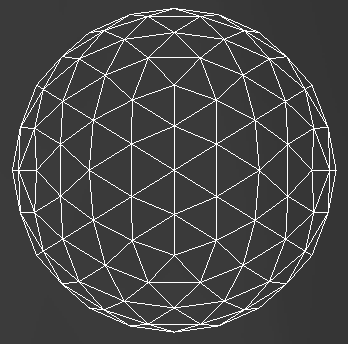
\includegraphics[width=0.4\linewidth, angle=0]{figs/Exemplos_QBall_visualizacao/MeshEsfericoIco.png}
        \caption{Malha Esférica a partir de duas subdivisões de um icosaedro. Esta malha possui 216 vértices não-colineares}
    \label{fig::MalhaEsferico}
 %   \hspace{1pt}
\end{figure}

\todo[inline]{Está confuso. Quem propôs usar icosaedro?}
\sout{A motivação da escolha desta categoria de malha esférica consiste em uma distribuição mais uniforme dos pontos na esfera em comparação a outras abordagens. Comparando com a malha gerada partir de discretizações nas coordenadas esféricas $(\phi, \theta)$, a distribuição de pontos é mais concentrada de pontos nos polos e mais esparsa no equador. Esta categoria de malha é referenciada em trabalhos da área como base de amostras para descrever funções esféricas \cite{TuchQBall2004, descoteaux2007_QBI, yeh2010}.}

\todo[inline]{Procure conectar as partes do seu texto. Ligue o "cômputo" com a Equação que você apresentou antes.}

\sout{A abordagem de implementação consiste no cômputo de todas as ODFs} Para cada \textit{voxel} do DWI\textcolor{red}{, todas as funções de distribuição de orientação (ODFs) foram computadas} para \textcolor{red}{todas} as direções representadas na malha com uso da Equação \ref{???} e \sout{seu armazenamento}\textcolor{red}{foram armazenadas} na memória para posterior uso na tractografia e geração de glifos.


\section{Renderização de funções de distribuição de orientação}

%Foi implementado um esquema de visualização para ODFs em glifos de acordo através de representações gráficas polares esféricas. A implementação serviu primeiramente para prova de conceito e posteriormente otimizada para que seja possível a sua renderização, \textit{voxel} a \textit{voxel}, em tempo interativo pelo VMTK-Neuro, o que foi possível nos testes feitos em um Macbook Pro Retina 13', com processador Intel Core i5 Dual-Core 2.7Ghz, processador gráfico Intel Iris Graphics 6100 1536 MB e memória RAM de 8 GB 1867 MHz DDR3.

\todo[inline]{Fazer uma breve justificativa da relevância da visualização das ODFs no contexto da sua proposta de uma visualização interativa almejando uma tractografia mais próxima dos tratos reais.}

\subsection{Plotagem polar esférica}

Como descrito na seção \ref{sec::trabalhos_relacionados_glifos}, a forma do glifo consiste na modulação do raio na direção $\mathbf{u}$ de uma malha esférica de acordo com uma versão normalizada do seu valor de imagem na função $\psi(\mathbf{u})$. A normalização que fizemos neste trabalho para representação está representado na equação \ref{eq::normglifo2}.

\begin{equation}
\label{eq::normglifo2}
    R(\mathbf{u}) = \frac{\psi(\mathbf{u}) - min(\psi(\mathbf{u}))}{max(\psi(\mathbf{u})) - min(\psi(\mathbf{u}))}
\end{equation}

As cores dos glifos consistem em um mapeamento das coordenadas dos vértices $(x_v,y_v,z_v)$ da malha esférica para as suas componentes RGB de acordo com a equação \ref{eq::cor_glifo} e ilustrado nos glifos da figura \ref{fig::glifo_ilustrado}. Esta forma de mapear, além de simples, entra muito em acordo com a codificação em cores definidos no mapa de FA e faz o entendimento do glifo ser intuitivo. %\todo{É imprescincível adicionar esta informação?}\sout{Não foi implementado o cômputo de vetores normais à superfície representadas pelo glifo, que consequentemente não tem iluminação associada.}

\begin{equation}
\label{eq::cor_glifo}
    (r,g,b) = (|x_v|,|y_v|,|z_v|)
\end{equation}

\begin{figure}[ht]

%\subfigcapskip = -5pt
    \centering
    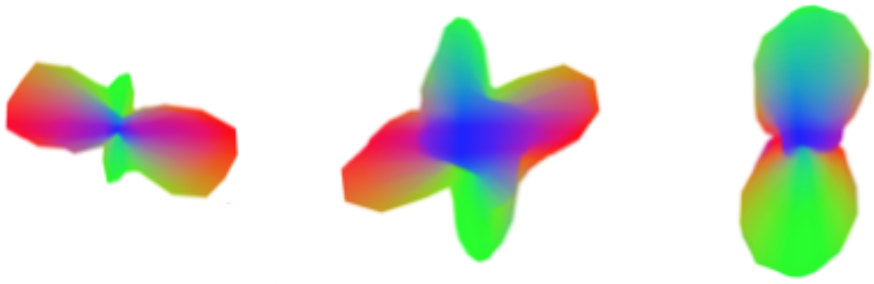
\includegraphics[width=.8\linewidth, angle=0]{figs/Esquema_Glifo/Glifos3Ex.png}
    \caption{Exemplos de glifos rasterizados de perfis de difusão que consistem em uma malha esférica modulada através da equação \ref{eq::normglifo2} e com as cores de acordo com a equação \ref{eq::cor_glifo}}
    \label{fig::glifo_ilustrado}
   \hspace{1pt}
\end{figure}

%\subsection{\sout{Abordagem de renderização}}

%\sout{\citeonline{peeters2009} apresentou pela primeira vez um esquema de renderização para esta categoria de glifos, nos quais são aperfeiçoados por \citeonline{peeters2011} e \citeonline{hlawitschka2012}. Estes esquemas utilizam a abordagem \textit{raycasting}.}

%\sout{No VMTK-Neuro, um dos algoritmos de renderização do tensor difusão por glifos superquádricos é feita por instanciações de uma malha esférica, no qual é customizada por parâmetros particulares a cada tensor de difusão referentes a cada \textit{voxel} detectado e posicionado na cena de acordo. Este esquema de renderização desenha os glifos em tempo interativo.}

%\sout{Pela maior simplicidade e boa efetividade da renderização por instanciações de uma malha esférica, o esquema desenvolvido neste trabalho utiliza esta abordagem.}



%Dados relativos ao desempenho \sout{serão mais detalhados na dissertação de mestrado}\textcolor{blue}{estão disponíveis no link ...}.



%\sout{Medições do tempo relativo ao desempenho foram feitas para a quantidade de 197 vértices da malha esférica \sout{em um}\textcolor{blue}{num} volume de resolução 128x128x90. Para uma quantidade na faixa de 5000 glifos renderizados simultaneamente sobre uma fatia completa, obtemos tem um tempo de resposta entre 80 e 110ms. Para uma quantidade pequena de glifos na faixa das dezenas, o tempo de resposta cai para o intervalo entre 60 e 70ms. Esse tempo de resposta está nas proximidades ou é menor do que o tempo de 0,1s, que é o limite máximo para que o usuário tenha a percepção de resposta instantânea da máquina e que suas ações são a causa de que algo aconteça na tela \cite{nielsen1994}.}

%\sout{No cômputo das ODFs do \textit{QBall}, é feito o mapeamento do sinal de DWI para a ODF a partir das direções derivadas da malha esférica. O glifo para visualização é gerado diretamente de acordo a representação gráfica polar esférica em que $R(\textbf{u}) = \psi(\mathbf{u})$, onde \textbf{u} é a direção de difusão. A malha esférica utilizada para geração dos glifos em \ref{section::QBall_Glifos} está representada na figura \ref{fig::MalhaEsferico}.}

%A priori, todas as ODFs são calculadas e normalizadas para o intervalo $[0,1]$ para cada um dos \textit{voxels} do volume e referenciadas no processo de renderização.

%O formato de armazenamento dos valores ODF associados à malha consiste numa lista de valores escalares associados a cada um dos \textit{voxels}.



%\todo[inline]{Falta uma descrição melhor de como são construídos os glifos a partir de ODFs e o seu mapeamento às entidades gráficas. Isso torna difícil o entendimento da sua implementação. !!Descrito em trabalhos relacionados!}
\subsection{Renderização de objetos}

A abordagem utilizada para renderização consiste em instanciações de uma malha esférica de N vértices centrada na origem e raio unitário, que é enviada à GPU uma única vez e sem repetição de vértices nos seus dados. A cada instância, a malha é transformada por uma matriz de translação e as suas amostras de ODF.

A matriz de translação posiciona o centro da malha esférica para a sua respectiva posição. O perfil de difusão diz respeito às ODFs particulares a cada glifo, que determina a forma do glifo através da multiplicação do vértice da malha associada à direção de difusão ao seu valor de ODF.

Estes elementos são enviados da CPU à GPU a cada requisição de desenho que tem como entrada uma lista de matrizes de translação e de amostras de ODF. Então, para atingirmos o objetivo da interatividade, é desejável que o tráfego de dados entre as partes seja o mínimo possível e sem redundância na descrição do objeto.

O envio do conjunto de coordenadas de translação à GPU consiste no envio de um vetor contendo P matrizes de translação como um atributo, que é único para cada malha esférica instanciada.

Os dados relativos a ODF enviados para GPU consistem nas N amostras referentes ao perfis de difusão para cada um dos P glifos a serem desenhados. A forma que as amostras de ODF são enviadas à GPU consiste na construção e envio de uma matriz $\mathbf{\Psi}_{PxN}$, onde P é a quantidade de glifos a serem desenhados e N consiste na quantidade de amostras de ODF utilizada. O envio da matriz $\mathbf{\Psi}$ à GPU é feito como uma textura 2D. 

Na matriz $\mathbf{\Psi}$, o elemento da i-ésima linha na j-ésima coluna da matriz se refere à ODF do i-ésimo glifo a ser desenhado associado ao j-ésimo vértice da esfera, que por sua vez tem as coordenadas da direção $\mathbf{u}_j$. Chamaremos  a ODF na i-ésima linha de $\psi_i(\mathbf{u})$ e o seu valor no j-ésimo vértice da esfera de $\psi_i(\mathbf{u}_j)$.

A recuperação na GPU das ODFs é feita através dos índices de instância e vértice. Para isto, é necessário que o índice de vértice (\textit{gl\_VertexID}\footnotemark) da direção de cada um dos vértices correspondam à coluna do seu respectivo valor de ODF $\psi(\mathbf{u}_j)$ na matriz de perfis de difusão. O acesso das linhas da matriz de perfis de difusão, correspondentes aos perfis de difusão de um \textit{voxel} é acessível pelo índice de instância (\textit{gl\_InstanceID}\footnotemark[\value{footnote}]). Tendo os dados organizados desta maneira estabelecida, o acesso é feito no \textit{vertex shader} utilizando através da função \textit{texelFetch}\footnotemark[\value{footnote}] com os argumentos de acesso de linha e coluna através do par (\textit{gl\_VertexID}, \textit{gl\_InstanceID})\footnotemark[\value{footnote}]\footnotetext{Todos os comandos foram implementados em OpenGL com a linguagem para \textit{shader} GLSL.}. A forma de acesso na GPU da matriz de perfis é ilustrada na figura \ref{fig::GPU2glifoGeneral}.

\begin{figure}[h]
%\subfigcapskip = -5pt
    \centering
    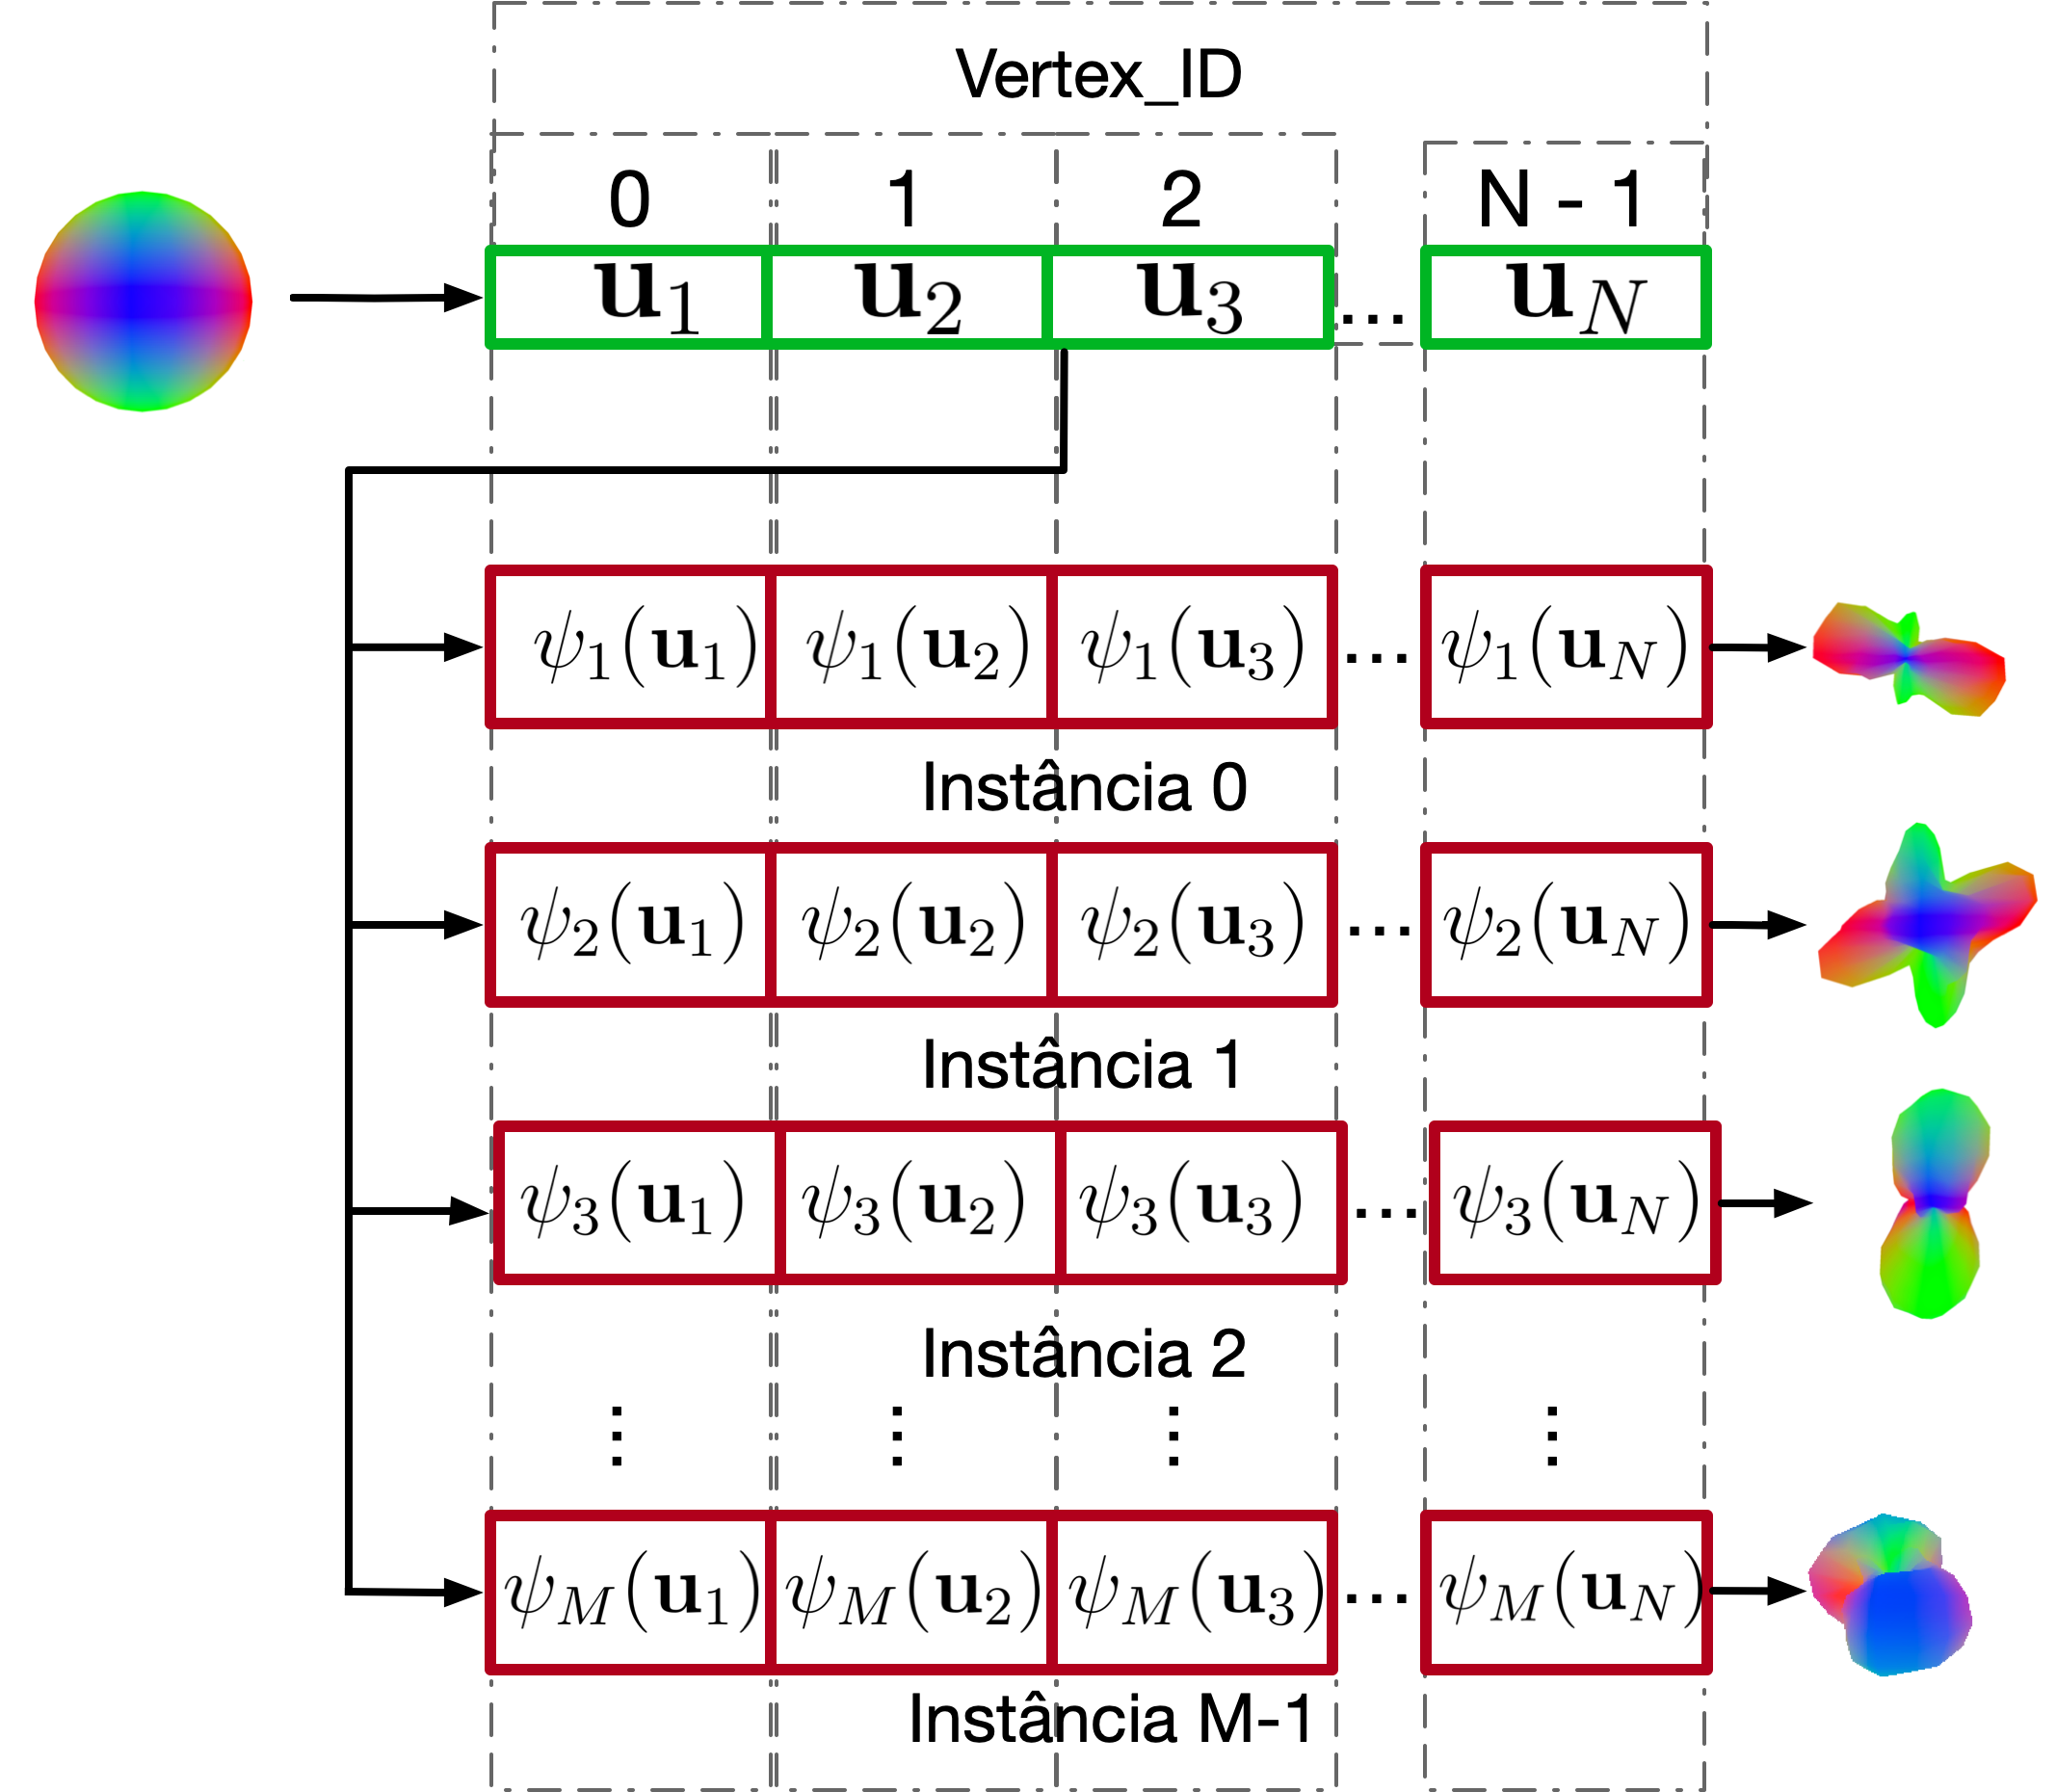
\includegraphics[width=.8\linewidth, angle=0]{figs/Esquema_Glifo/GPU2GlifoGeneral.png}
    \caption{Ilustração da organização de dados na GPU da matriz de perfil de difusão (vermelho). Os vértices da malha esférica estão em verde. A cada instância, a customização do glifo se dá através da multiplicação do vértice da malha com o seu respectivo valor $\psi$, recuperado no \textit{vertex shader} através do seu índice de vértice para os P glifos a serem renderizados.}
    \label{fig::GPU2glifoGeneral}
   \hspace{1pt}
\end{figure}


%A figura \ref{fig::organizacao2GPU} ilustra \todo{Não entendi ... a organização é dinâmica? Isso é muito custoso!}\textcolor{brown}{a organização dos dados para quando ocorre a detecção de quatro \textit{voxels}}.

%Na GPU, a malha esférica, copiada anteriormente e alocada em um \textit{vertex buffer object} (VBO), é instanciada P vezes. A recuperação na GPU das ODFs é feita através dos índices de instância e vértice. Para isto, é necessário que o índice de vértice (\textit{gl\_VertexID}\footnotemark) da direção de cada um dos vértices correspondam à coluna do seu respectivo valor de ODF $\psi(\mathbf{u})$ da matriz de perfis de difusão. O acesso das linhas da matriz de perfis de difusão, correspondentes aos perfis de difusão de um \textit{voxel}acessível pelo índice de instância (\textit{gl\_InstanceID}\footnotemark[\value{footnote}]). Tendo os dados organizados desta maneira estabelecida, o acesso é feito no \textit{vertex shader} utilizando através da função \textit{texelFetch}\footnotemark[\value{footnote}] com os argumentos de acesso de linha e coluna através do par (\textit{gl\_VertexID}, \textit{gl\_InstanceID})\footnotemark[\value{footnote}]\footnotetext{Todos os comandos foram implementados em OpenGL com a linguagem para \textit{shader} GLSL.}. A forma de acesso na GPU da matriz de perfis é ilustrada na figura \ref{fig::GPU2glifoGeneral}.

A cor dos glifos é definida de acordo com o vértice da malha esférica instanciada no \textit{vertex shader} e definida de acordo com a equação \ref{eq::cor_glifo}.



\todo[inline]{Incluir os pseudocódigos de shaders não ajudaria o entendimento da ideia?}



\subsection{Integração ao VMTK-Neuro}

No VMTK-Neuro, são computados a priori o conjunto de amostras de ODFs para uma determinada malha esférica e de matrizes de translação associados a cada um dos voxels.

Há um sistema de detecção de amostras do DWI aparentes na cena integrado ao VMTK-Neuro, tanto na renderização de fatias, quanto na renderização do volume em três dimensões.

Na renderização de fatias, a inferência dos \textit{pixels} aparentes na tela consiste na leitura dos índices do \textit{voxel} nas fatias coronais, axiais no qual os glifos são posicionados de acordo com a posição do seu respectivo \textit{pixel}.

Na renderização tridimensional, também há uma funcionalidade para detecção de amostras aparentes. A detecção é baseada em \textit{raycasting} computado sobre o volume na GPU, no qual foi proposto e implementado no VMTK-Neuro por \citeonline{raphael_dissertacao}. Cada uma das amostras é associado a uma matriz de translação pré-computada para o seu centro no 3D.

A partir de $P$ \textit{voxels} detectados em uma requisição de desenho, suas respectivas matrizes de posicionamento são copiadas e armazenadas como um vetor e enviadas à GPU. Da mesma maneira, a matriz $\Psi$ é computada a partir das amostras detectadas e enviada à GPU, conforme mostrado na Figura \ref{fig::organizacao2GPU}.


\begin{figure}[ht]

%\subfigcapskip = -5pt
    \centering
    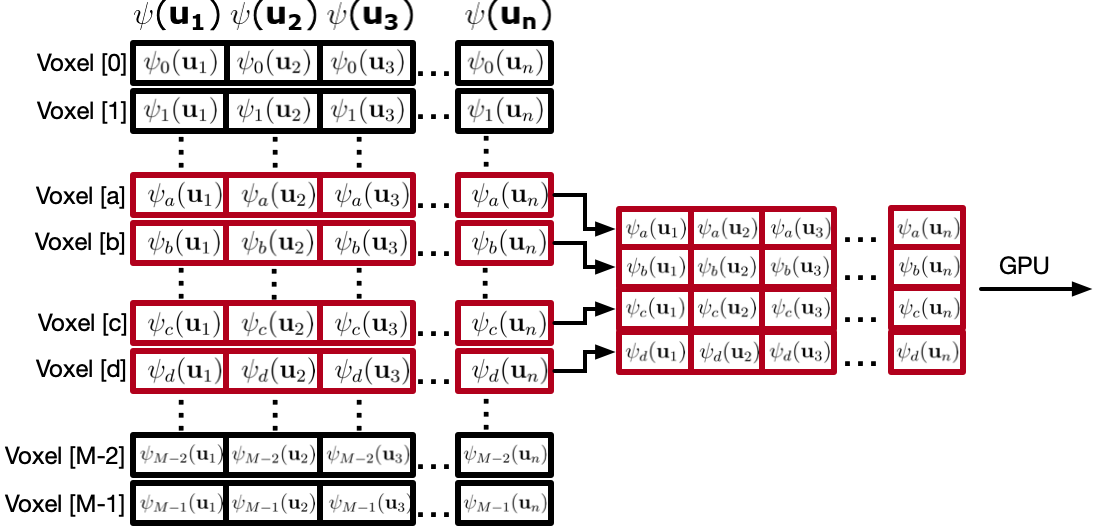
\includegraphics[width=1.000\linewidth, angle=0]{figs/Esquema_Glifo/organizacao2GPU.png}
    \caption{Ilustração da organização de dados de perfis de difusão antes do envio à GPU. Em vermelho, estão os perfis de difusão de P voxels detectados \textit{voxels} ($d_1$, $d_2$, ..., $d_P$) detectados, não necessariamente em sequência na memória, que são copiados para uma matriz e enviados à GPU. O valor S corresponde a quantidade voxels do volume e $N$ se refere a quantidade de amostras nos perfis de difusão}
    \label{fig::organizacao2GPU}
   \hspace{1pt}
\end{figure}


Há elementos comuns a todos os glifos, que são enviados à GPU como variáveis uniformes. Estes elementos se referem a parâmetros de câmera na cena e a transformações relativas a orientação neurológica, que integram a matriz \textit{model-view-projection} e fator de escala.

As transformações relativas à orientação configuram a visualização de fatias para que fique compatível com um dos sistemas de orientação, que são a neurológica (LAS) e radiológica (RAS). O fator de escala é função do \textit{zoom} aplicado e dimensão do \textit{voxel}.





%O envio do conjunto de matriz de reposicionamento à GPU consiste no envio das coordenadas de translação como um atributo, que é único para cada malha esférica instanciada. Estes dados são armazenados \sout{por}\textcolor{red}{em} um \todo{Corresponde a qual objeto gráfico na GPU?}vetor, cujo índice se refere ao deslocamento da malha instanciada para seu respectiva posição.



%\subsection{\sout{Esquema de }Renderização na GPU}

%\todo[inline]{Para que o texto seja auto-contido, ou você referencia o trabalho do Raphael ou faz uma descrição completa para que o algoritmo seja reprodutível. Pois pelo que entendi, a sua proposta é uma variante da proposta do Raphael. É preciso deixar bem claro onde está a variação. O algoritmos é para GPU? Quantos passos são executados? Quais shaders?}

%A abordagem utilizada para renderização consiste em instanciações de uma malha esférica de N v centrada na origem e raio unitário, que é enviada à GPU uma única vez e sem repetição de vértices nos seus dados. A cada instância, a malha é transformada por duas classes de elementos: os elementos em comum a todos os \textit{voxels} e os particulares.

%O envio do conjunto de matriz de reposicionamento à GPU consiste no envio das coordenadas de translação como um atributo, que é único para cada malha esférica instanciada. Estes dados são armazenados \sout{por}\textcolor{red}{em} um \todo{Corresponde a qual objeto gráfico na GPU?}vetor, cujo índice se refere ao deslocamento da malha instanciada para seu respectiva posição.

%\todo[inline]{Suportar visualizações em LAS e RAS é uma demanda clínica e não por uma adequação ao VMTK ... }
%Os elementos comuns se referem às rotações e mudanças de escala. O fator de escala, que é função do \textit{zoom} aplicado e dimensão do \textit{voxel}, bem como o cômputo das transformações relativas à orientação, para que fiquem compatíveis com os sistemas de orientação neurológica (LAS) e radiológica (RAS) constam no VMTK-Neuro.% e sincronização com fatias bidimensionais.

%Há dois elementos particulares que customizam os glifos, cujos dados são enviados à GPU a cada \textit{frame} após os voxels aparentes na cena serem detectados. O primeiro é a translação para reposicionamento, que desloca a malha para o centro do seu respectivo \textit{voxel} e o segundo diz respeito às ODFs particulares a cada \textit{voxel}, que determina a forma do glifo através da multiplicação do vértice da malha associada à direção de difusão ao seu valor de ODF. %A implementação da matriz de reposicionamento foi algo direto, sendo uma adaptação do algoritmo dos glifos para DTI, pois o deslocamento é comum a todos os vértices instanciados. Já o mesmo não acontece com o mapa de ODFs.

%Para atingirmos o objetivo da interatividade, é necessário que o tráfego de dados CPU-GPU seja o mínimo possível e sem redundância. A maior parte deste tráfego se refere aos elementos particulares. Estes elementos são enviados à GPU a cada \textit{frame} de acordo com os \textit{voxels} visíveis detectados.

%\todo[inline]{Passou todos os dados para GPU como textura?}
%Os de ODF sim. Os de translação, não

%O envio do conjunto de matriz de reposicionamento para à GPU consiste na cópia de dados de deslocamento pré-computados para os \todo{Quais são os voxels detectados?}\textit{voxels} detectados. Estes dados são armazenados \sout{por}\textcolor{red}{em} um \todo{Corresponde a qual objeto gráfico na GPU?}vetor, cujo índice se refere ao deslocamento da malha instanciada para seu respectiva posição.

%O envio dos dados de ODF para GPU consiste na cópia dos dados referentes aos \textit{voxels} detectados de cada valor para cada perfil de difusão \todo{?}\textcolor{brown}{adotada consiste} na cópia dos dados de ODF para uma matriz pxn, onde p é a quantidade de \textit{voxels} detectados e n consiste na quantidade de amostras de ODF. A i-ésima linha da matriz se refere ao perfil de difusão do i-ésimo \textit{voxel} detectado, enquanto a j-ésima coluna se refere ao valor de difusão associado ao $\mathbf{u}_j$ para todos os \todo{Quais são os voxels detectados?}\textit{voxels} detectados. Esta matriz é enviada à GPU como uma textura 2D. A figura \ref{fig::organizacao2GPU} ilustra \todo{Não entendi ... a organização é dinâmica? Isso é muito custoso!}\textcolor{brown}{a organização dos dados para quando ocorre a detecção de quatro \textit{voxels}}.



%\todo[inline]{Incluir os pseudocódigos de shaders não ajudaria o entendimento da ideia?}

%Na GPU, a malha esférica, copiada anteriormente e alocada em um \todo{VBO?}\textit{buffer}, é instanciada P vezes. Para a recuperação na GPU do perfil de difusão, é necessário que índice de vértice (\textit{gl\_VertexID}\footnotemark) da direção de cada um dos vértices correspondam à coluna do seu respectivo valor de ODF $\psi(\mathbf{u})$ da matriz de perfis de difusão. O acesso das linhas da matriz de perfis de difusão, correspondentes aos perfis de difusão de um \textit{voxel}acessível pelo índice de instância (\textit{gl\_InstanceID}\footnotemark[\value{footnote}]). Tendo os dados organizados desta maneira estabelecida, o acesso é feito no \textit{vertex shader} utilizando através da função \textit{texelFetch}\footnotemark[\value{footnote}] com os argumentos de acesso de linha e coluna através do par (\textit{gl\_VertexID}, \textit{gl\_InstanceID})\footnotemark[\value{footnote}]\footnotetext{Todos os comandos foram implementados em OpenGL com a linguagem para \textit{shader} GLSL.}. A forma de acesso na GPU da matriz de perfis de difusão como uma textura 2D é mostrada na figura \ref{fig::GPU2glifoGeneral}.


%\begin{figure}[h]
%%\subfigcapskip = -5pt
%    \centering
%    \includegraphics[width=.8\linewidth, %angle=0]{figs/Esquema_Glifo/GPU2Glifo%.png}
%    \caption{Ilustração da organização de %dados na GPU da matriz de perfil de %difusão (vermelho) enviados conforme %mostrado na figura %\ref{fig::organizacao2GPU}. Os %vértices da malha esférica estão em %verde. A cada instância, a %customização do glifo se dá através %da multiplicação do vértice da malha %com o seu respectivo valor $\psi$, %recuperado através do seu índice de %vértice.}
%    \label{fig::GPU2glifo}
%   \hspace{1pt}
%\end{figure}

\subsection{Resultados}

%\todo[inline]{Comentar que, para aproveitar as funcionalidades de interações gráficas disponíveis no VMTK-Neuro, o algoritmo foi integrado no VMTK-Neuro. Se puder, comentar os pontos de conexão.}

Na seção \ref{section::QBall_Glifos} do apêndice, seguem algumas imagens dos glifos derivados de ODFs integrados ao VMTK-Neuro. O volume é derivado da competição ISMRM \cite{TractometerTool}. A malha esférica utilizada é a mesma da figura \ref{fig::MalhaEsferico}.

Medições do tempo relativo ao desempenho foram feitas para a quantidade de 197 e 422 vértices da malha esférica para diferentes quantidades de glifos renderizados e estão anotados nas tabelas \ref{tab::benchmark_glifos_197} e \ref{tab::benchmark_glifos_422}. O computador utilizado para o \textit{benchmark} foi um Macbook Pro Retina 13', com processador Intel Core i5 Dual-Core 2.7Ghz, processador gráfico Intel Iris Graphics 6100 1536 MB e memória RAM de 8 GB 1867 MHz DDR3.

Os resultados estão também anotados como fração do limite de tempo de reação instantânea ($t_{max}$). Seja $t$ o intervalo de tempo entre a interação do usuário com um sistema e a sua respectiva resposta, mostrada de forma visual. O tempo $t_{max}$ é o limite máximo de $t$ em que o usuário tenha a percepção que o sistema reage instantaneamente as suas ações que, de acordo com \citeonline{nielsen1994}, é de 0,1s.

%\citeonline{nielsen1994} define o tempo de 0,1s 
%\todo{Não entendi ...}\textcolor{brown}{e que suas ações são a causa de que algo aconteça na tela }. 

%\todo[inline]{Percebeu oscilações nos tempos. A variação não é linear. Vamos ter que tentar entender por quê esta contra-intuitivo comportamento.}

O resultados mostrados nas tabelas \ref{tab::benchmark_glifos_197} e \ref{tab::benchmark_glifos_422} mostram que centenas de glifos podem ser renderizados na faixa de centenas de microssegundos e unidades de milissegundos, o que possibilita a sua integração a esquemas de renderização mais complexos e custosos computacionalmente relacionados a volumes de difusão.

%\todo[inline]{O que é fração do limite máximo para interatividade?}
\pagebreak

%Pode-se notar que em ambas as malhas esféricas utilizadas, a fração de tempo de execução é pequena para centenas







%A estratégia adotada para superar esse problema foi o  armazenamento dos dados de ODF dos \textit{voxels} detectados e o envio para GPU como uma textura 2D, onde é possível acessar os dados de ODF de acordo com índices de instância (relativo ao \textit{voxel}) e o índice de vértice (relativo à malha esférica instanciada na GPU), que requer uma organização específica para os dados enviados a cada \textit{frame}.

%O problema no valor de ODFs é que não há parâmetros em comum entre vértices da mesma esfera instanciada. A API OpenGL e a linguagem GLSL não oferecem formas diretas de se fazer alocação dinâmica de memória na GPU, em que disponibilize N*M valores de ODF para N \textit{voxels} aparentes na tela e uma malha esférica de M vértices.

%\todo[inline]{Como foi a estruturação na textura? Procurou explorar a coalescência/a sequência de acessos?}
%Evidentemente que há um mapeamento do domínio $[0,1]^2$, que é padrão numa unidade de textura, para a quantidade de instâncias e vértices que são processados.

%\todo[inline]{Há alguma explicação plausível para a queda de tempo na GPU entre 30 e 100 e entre 2000 e 5000?}
\begin{table}[H]
\begin{tabular}{c|c|c|c|c}
\textbf{\begin{tabular}[c]{@{}c@{}}Quantidade \\ de glifos\end{tabular}} & \textbf{\begin{tabular}[c]{@{}c@{}}Organização \\ e envio de \\ dados à GPU\\ ($\mu$s)\end{tabular}} & \textbf{\begin{tabular}[c]{@{}c@{}}Processamento\\ na GPU e \\ desenho ($\mu$s)\end{tabular}} & \textbf{\begin{tabular}[c]{@{}c@{}}Tempo de \\ execução\\ ($\mu$s)\end{tabular}} & \textbf{\begin{tabular}[c]{@{}c@{}}Fração do limite \\ máximo para\\ interatividade\end{tabular}} \\ \hline
30                                                                       & 139.97                                                                                                 & 2097.00                                                              & 2236.97                                                                        & 2\%                                                                                               \\
100                                                                      & 190.72                                                                                                 & 517.00                                                               & 707.72                                                                         & 1\%                                                                                               \\
500                                                                      & 387.25                                                                                                 & 745.00                                                               & 1132.25                                                                        & 1\%                                                                                               \\
2000                                                                     & 1352.93                                                                                                & 792.00                                                               & 2144.93                                                                        & 2\%                                                                                               \\
5000                                                                     & 4768.94                                                                                                & 435.00                                                               & 5203.94                                                                        & 5\%                                                                                               \\
10000                                                                    & 11886.44                                                                                               & 7798.00                                                              & 19684.44                                                                       & 20\%                                                                                             
\end{tabular}
\caption{\textit{Benchmark} de glifos representados por uma malha esférica de 197 vértices}
\label{tab::benchmark_glifos_197}
\end{table}


%\todo[inline]{Por quê a queda de tempo quando passa de 30 para 100? Alguma justificativa plausível?}
\begin{table}[H]
\begin{tabular}{c|c|c|c|c}
\textbf{\begin{tabular}[c]{@{}c@{}}Quantidade \\ de glifos\end{tabular}} & \textbf{\begin{tabular}[c]{@{}c@{}}Organização \\ e envio de \\ dados à GPU\\ ($\mu$s)\end{tabular}} & \textbf{\begin{tabular}[c]{@{}c@{}}Processamento\\ na GPU e \\ desenho ($\mu$s)\end{tabular}} & \textbf{\begin{tabular}[c]{@{}c@{}}Tempo de \\ execução\\ ($\mu$s)\end{tabular}} & \textbf{\begin{tabular}[c]{@{}c@{}}Fração do limite \\ máximo para\\ interatividade\end{tabular}} \\ \hline
30                                                                       & 270.40                                                                                               & 2174.00                                                              & 2444.40                                                                          & 2\%                                                                                               \\
100                                                                      & 244.93                                                                                               & 447.00                                                               & 691.93                                                                           & 1\%                                                                                               \\
500                                                                      & 724.67                                                                                               & 725.00                                                               & 1449.67                                                                          & 1\%                                                                                               \\
2000                                                                     & 5439.72                                                                                              & 3384.00                                                              & 8823.72                                                                          & 9\%                                                                                               \\
5000                                                                     & 13914.25                                                                                             & 5094.00                                                              & 19008.25                                                                         & 19\%                                                                                              \\
10000                                                                    & 26841.13                                                                                             & 4773.00                                                              & 31614.13                                                                         & 32\%                                                                                             
\end{tabular}
\caption{\textit{Benchmark} de glifos representados por uma malha esférica de 422 vértices}
\label{tab::benchmark_glifos_422}
\end{table}

\textcolor{red}{\chapter{Extração de Direções Plausíveis de Fibras}}

\todo[inline]{Tenho impressão de que você mistura técnica com dados no texto. Preste atenção.}

\textcolor{red}{O procedimento para reconstrução de uma fibra não está, de fato, atrelado aos perfis de difusão, e sim às orientações das plausíveis fibras extraídas destes dados.} Descreveremos neste capítulo o processamento para extração de informações direcionais de ODFs computadas através do QBI para tractografia assim como o algoritmo de tractografia que utilizam estas informações direcionais para gerar linhas representativas de fibras do cérebro.


\todo[inline]{Sugiro discutir em separado a extração de picos, pois é um procedimento que de fato motivou este trabalho ... pelas suas experiências do estágio ...}

\todo[inline]{Antes de detecção de máximos, é necessário que os máximos sejam detectáveis. Como você melhorou as ODFs para que seus máximos sejam mais "concentrados"?}

O procedimento para extração de direções plausíveis de fibras se dá através da detecção de máximos locais em uma ODF $\psi(\mathbf{u})$\textcolor{red}{, pois foram confirmadas experimentalmente correspondências entre os picos das funções e as orientações das fibras \citeonline{Hess2006}.}

O processo de detecção de máximos locais é feito através das amostras de ODFs, no qual uma direção é classificada como máximo através da comparação com amostras vizinhas.

\todo[inline]{Segundo \citeonline{Aganj2009} as estimativas das funções ODF pela técnica original podem gerar distorções, os autores propõem um fator de correção para ter uma estimativa melhor de ODFs.}

Definimos a vizinhança de uma direção $\mathbf{x}$ para uma função esférica, discretizada em um conjunto finito de direções $\mathbf{U}$ como o conjunto $\mathbf{N_x}$, cujos elementos satisfazem as seguintes condições:

%Em funções esféricas, para um conjunto discreto de direções no domínio $\mathbf{U}$, definimos a vizinhança de uma direção $\mathbf{u}$ como o conjunto de vetores unitários $\mathbf{N_u}$ de acordo com a equação \ref{eq::neighboorhood}.

\begin{equation}
\label{eq::neighboorhood}
    \mathbf{N_x} = \{\mathbf{s} \in \mathbf{U}  | \mathbf{x}.\mathbf{s} > \cos{\theta_{thr}} \}
\end{equation}

onde $\theta_{thr}$ é o ângulo máximo entre duas amostras direcionais para serem consideradas vizinhas. A escolha do $\theta_{thr}$ leva em consideração a quantidade de pontos do domínio $\mathbf{U}$ utilizado.

A direção $\mathbf{x}$ é considerado máximo local de $\psi(\mathbf{u})$ se $\psi(\mathbf{x}) > \psi(\mathbf{s}) \; \forall \; \mathbf{s} \in \mathbf{N_x}$.



\chapter{Tractografia em tempo real baseado em picos}

Neste capítulo descreveremos o algoritmo de tractografia baseado em picos. Na seção \ref{sec::decisoesiniciais_tractografia}, apresentamos condições desejáveis para o algoritmo proposto, que consiste em \todo{Releia ... impossível entender.}\textcolor{brown}{resolver tratos que algoritmos de tractografia baseadas em métodos HARDI resolvem, ter um baixo custo computacional e gerar visualmente resultados que estejam correlacionados ao trato de interesse}.

\sout{Descreveremos neste capítulo o processamento para extração de informações direcionais de ODFs computadas através do QBI para tractografia assim como o algoritmo de tractografia que utilizam estas informações direcionais para gerar linhas representativas de fibras do cérebro.}

Para validação do algoritmo, iremos compará-lo com a abordagem DTI, \todo{Releia ...}\textcolor{brown}{com o estado da arte, que está aplicativo MRTrix (https://www.mrtrix.org) \cite{tournier2019} no trato corticoespinhal}. Para validação de performance, também apresentaremos o \todo{Qual?}seu \textit{benchmark}.

\sout{Ressaltamos que o algoritmo de tractografia a ser apresentado não está atrelado a método de imageamento e sim a informações direcionais extraídas destes métodos, sendo o QBI o método utilizado para este fim.}


\section{\textit{Q-Ball} e direções de fibras}

%\subsection{Extração de picos}

!!Detalhar extração de picos.

!!Mostrar Linhas representativas coloridas em um mapa FA e comparar com os glifos.

\section{Tractografia}

\subsection{Formulação}

Com a restrições mencionadas no início deste capítulo, o trabalho consiste na adaptação de um dos dois algoritmos de tractografia determinísticos propostos por \citeonline{descoteaux2007}. \sout{O algoritmo, chamado de dODF-STR, gera um \textit{streamline}, cujo processo é feito na escolha de uma e somente uma direção baseado nos picos extraídos de uma ODF. Em comparação com a outra abordagem proposta, chamada de SPLIT-STR, gera bifurcação dos \textit{streamlines} para múltiplas direções extraídas do modelo.}

\sout{
\citeonline{descoteaux2007} propõem um pré-processamento que consiste no afiamento da ODF, na qual visa prover um maior destaque aos picos e regiões de mais alta magnitude na ODF, conforme a figura \ref{fig::sharpening}. Com dados artificiais, o autor faz um experimento no qual a extração de direção de fibras é feito com a ODF de difusão extraída do QBI, a ODF após o processamento, a função de distribuição de orientação de fibra extraída do método deconvolução esférica filtrada para diferentes relações sinal ruído. O resultado do experimento atesta que a precisão da extração de picos aumenta com o pré-processamento, e tem um grau parecido com a abordagem de deconvolução esférica. Este pré-processamento não foi contemplado neste trabalho de mestrado.
}

%O algoritmo proposto consiste em um pré-processamento, em que consiste no afiamento da ODF, no qual visa prover um maior destaque aos picos e regiões de mais alta magnitude na ODF, conforme a figura \ref{fig::sharpening}. Após o pré-processamento, assim como na abordagem DTI determinística, a tractografia visa gerar linhas representativas de fibras do cérebro utilizando um modelo como base, que neste caso são ODFs.


\begin{figure}[h]
%\subfigcapskip = -5pt
    \centering
    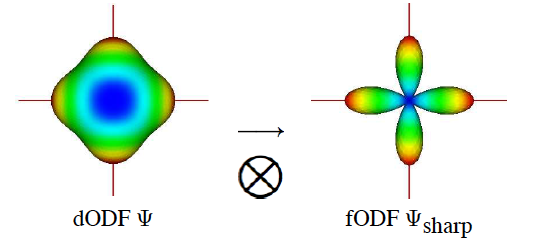
\includegraphics[width=.45\linewidth, angle=0]{figs/Tractografia/sharpening.png}
     \caption{Operação de afiamento de ODF. A função esférica a esquerda mostra um glifo de ODF obtida através de um sinal HARDI simulado e a direita a sua transformação em uma ODF afiada. \\
     Fonte: \cite{descoteaux2007}
     }
     \label{fig::sharpening}
 %   \hspace{1pt}
\end{figure}

\sout{
Evidentemente que não é possível fazer uma tractografia que computa tratos em tempo interativo com uma abordagem idêntica como \citeonline{descoteaux2007}, que a cada iteração interpola trilinearmente 1281 amostras de ODF para computar picos no processo de decisão da direção do passo da curva em um \textit{loop}.
}

\sout{
A estratégia adotada então para este impasse é similar ao proposto por \citeonline{Chamberland2016}, que consiste em computar informações de direções de fibras na sua totalidade antes da execução da tractografia. Estes dados são acessados na tractografia e nas regiões \textit{intra-voxel}, a estimativa das direções é feita através da interpolação pelo vizinho mais próximo.
}

Para atenuar o erro gerado pela atribuição do vizinho mais próximo, adotamos uma estratégia de aumentar as amostras de ODF para extração de informações direcionais neste respeito utilizando interpolação trilinear. Os resultados apresentados !!(na seção???) utilizam picos de um volume com a resolução duplicada nas direções x, y, z (de 2x2x2 $mm^3$ para 1x1x1 $mm^3$).

\sout{
Uma questão pertinente acerca do aumento de amostras é se ela deve ser feita no DWI, no qual o método de difusão é aplicado sobre o volume super amostrado ou se pode ser feito diretamente nos valores de ODF. A literatura não é clara neste aspecto. !!Referencias!
}

O cômputo do passo na tractografia em um ponto pode ser categorizado em duas etapas: a escolha da direção de propagação e a equação do passo. A escolha da direção de propagação é feita a partir dos picos candidatos, no qual o escolhido é a direção que tem o menor ângulo com o passo anterior. Sobre a equação do passo, utilizaremos a adaptação que \citeonline{Chamberland2016} propôs como uma adaptação da equação do passo proposta por \citeonline{Weinstein1999} na tractografia baseada em DTI, exposta na equação \ref{eq::tractografia_weinstein}. A equação \ref{eq::tractografia_chamberland} mostra esta relação:

\begin{equation}
\label{eq::tractografia_chamberland}
    \mathbf{v}_{step} = A\mathbf{e} + (1 - A)(w_{punct}\mathbf{e} + (1-w_{punct})\mathbf{v}_{in})
\end{equation}

onde $\mathbf{v}_{step}$ é a direção de propagação da \textit{streamline}, $A$ é uma métrica de anisotropia (GFA), $\mathbf{e}$ é o pico escolhido dentre os candidatos no ponto em questão, $\mathbf{v}_{in}$ é a direção de propagação anterior e $w_{punct}$ é o parâmetro que pondera a decisão do passo continuar na direção anterior ou seguir na direção do pico escolhido, no caso em que a anisotropia do ponto seja baixa.

Acerca dos parâmetros referenciados na equação \ref{eq::tractografia_chamberland}, o GFA é uma métrica previamente calculada para todo o volume e seu valor nas regiões \textit{intra-voxels} são computados a partir de interpolação trilinear. O parâmetro $w_{punct}$, assim como exposto na seção \ref{ssec::tractografia_e_seletividade} é um parâmetro contido no intervalo [0, 1] e é configurável pelo usuário.

\subsection{Algoritmo e questões computacionais}

O algoritmo implementado de tractografia em função de uma semente está mostrado no pseudocódigo \ref{psc::tractography}. Os parâmetros de entrada consistem na semente inicial contida no DWI ($p_0$), limiares de ângulo e anisotropia ($\theta_{thr}$ e $t_{aniso}$), o parâmetro $w_{punct}$ da equação \ref{eq::tractografia_chamberland}, o sentido que o algoritmo de tractografia deverá tomar ($d_{inv} = -1$ para inverter ou $d_{inv} = 1$ para manter igual ao máximo local)\footnote{Funções representativas de difusão são funções pares ($\Psi(\mathbf{u}) = \Psi(\mathbf{-u})$). Por questões de memória, na nossa implementação, não armazenamos a mesma direção em sentidos opostos}  o tamanho do passo na integração de linhas ($s_{len}$) e a quantidade máxima de pontos nos tratos ($l_{max}$). O conjunto de pontos de saída é representado pelo conjunto $\mathbf{\Phi}$.

\todo[inline]{Sugiro que faça uma descrição do algoritmo, contendo referências às linhas de instrução. A descrição abaixo está difícil de entender e seguir o pseudo-código que você escreveu.}

As funções representadas no pseudocódigo são Valid(p) (linha \ref{alg:psc_valid}), que verifica se o ponto computado está dentro do domínio do volume , GFA(p) (linha \ref{alg::GFA}) consiste no cômputo do GFA no ponto p e ExtractLocalMaxSet(p) (linha \ref{alg::extractLocalMaxSet}) representa a escolha de picos da ODF no ponto p, no qual retorna um conjunto de vetores.




%!!O algoritmo implementado de tractografia em função de uma semente está mostrado no pseudocódigo \ref{psc::tractography} da tractografia ilustra o algoritmo a ser implementado, nos quais os candidatos a serem direções de propagação são retirados dos picos de ODF computados. Na abordagem dODF-STR, a direção escolhida é a que possui menor ângulo com a direção de propagação da curva, que é definida na iteração anterior, enquanto na outra abordagem, chamada pelo autor de SPLIT-STR, gera linhas derivadas dos múltiplos máximos locais detectados.

\begin{algorithm}
\caption{Integração de linhas em tractografia}
\label{psc::tractography}
\begin{algorithmic}[1]
\Function{tractography}{$p_0$, $\theta_{thr}$, $t_{aniso}$, $w_{punct}$, $d_{inv}$, $s_{len}$, $l_{max}$}
\State $\mathbf{\Phi} \gets \emptyset$
\State $p \gets p_0$
\State $\mathbf{d} \gets d_{inv}(argmax_\mathbf{u} \; \psi(\mathbf{u})_{p_0})$
%\State Insert $p$ in $\mathbf{\Phi}$
\State $\mathbf{\Phi} \gets \mathbf{\Phi} \cup  \{p\}$ 
\State $l \gets 1$
\While{$l < l_{max}$}
\State $p \gets p + s_{len} \mathbf{d}$
\State \textbf{If} $\neg$ Valid(p) \textbf{then} STOP \label{alg:psc_valid} %\EndIf 
\State \textbf{If} $\text{GFA}(p) < t_{aniso}$  \textbf{then} STOP \label{alg::GFA}%\EndIf
\State $\mathbf{M} = ExtractLocalMaxSet(p)$ \label{alg::extractLocalMaxSet}
\State $\mathbf{d}_{new} \gets argmax_{\textbf{m}} \; |\mathbf{d}.\mathbf{m}|, \; \mathbf{m} \in \mathbf{M}$
\State \textbf{If} $\mathbf{d}.\mathbf{d}_{new} < 0$  \textbf{then} $\mathbf{d}_{new} \gets -\mathbf{d}_{new}$%\EndIf
\State \textbf{If} $\mathbf{d}_{new}.\mathbf{d} < cos(\theta_{thr})$ \textbf{then} STOP%\EndIf
\State $\mathbf{d} \gets \text{GFA}(p)\mathbf{d}_{new} + (1 - \text{GFA}(p))(w_{punct}\mathbf{d}_{new} + (1 - w_{punct})\mathbf{d})$
\State $\mathbf{d} \gets \mathbf{d}/|\mathbf{d}|$
%\State Insert $p$ in $\mathbf{\Phi}$
\State $\mathbf{\Phi} \gets \mathbf{\Phi} \cup  \{p\}$
\State $l \gets l + 1$
\EndWhile
\State \Return $\mathbf{\Phi}$
\EndFunction
\end{algorithmic}
\end{algorithm}

\todo[inline]{Qual parte está no geometry shader???}
\textcolor{brown}{
Além disso, assim como a tractografia baseada em DTI no VMTK-Neuro, a implementação do algoritmo foi implementado na GPU, utilizando o \textit{geometry shader} na linguagem GLSL da API OpenGL, no qual o cômputo dos \textit{streamlines} em cada um dos dois sentidos possíveis, são paralelizados.
}

\todo[inline]{O que CUDA tem a ver com a sua implementação? Não entendi.}
\textcolor{brown}{
O ponto que motivou esta escolha vem da maior compatibilidade desta forma de implementação com o que há no mercado. O CUDA funciona somente para GPUs NVIDIA, e das ferramentas que funcionam em Linux, Windows e MacOS, há apenas OpenGL e OpenCL, no qual nosso grupo de pesquisa escolheu o OpenGL para computação na GPU. Devido a descontinuidade do OpenGL no MacOS na versão 4.1, que é o sistema operacional utilizado no desenvolvimento do trabalho, o \textit{compute shader} não está disponível como ferramenta e então foi escolhido o \textit{geometry shader} para este fim.
}

A parte de interface, relativas ao desenho de ROI e filtros tem sido adaptadas da tractografia por DTI, já integrada ao VMTK-Neuro, assim como parâmetros relativos aos critérios de parada devido a baixa anisotropia e angulação de direções consecutivas brusca.

\todo[inline]{Será que vai funcionar como você escreveu?}
\textcolor{brown}{
A representação na GPU das grandezas envolvidas são feitas na seguinte maneira: O mapa GFA é enviado à GPU como uma textura 3D e o conjunto de máximos locais encontrados como um vetor de texturas 3D, onde cada um dos vetores representa um conjunto de direções. Há um valor máximo configurável que diz respeito à quantidade de picos a ser enviados a GPU, que na nossa implementação limitamos em cinco. Pontos que possuem uma quantidade de picos menor que o máximo projetado tem os índices vagos representados como vetor nulo.
}


\section{Validação}

\subsection{Metodologia}

\subsection{Comparação com o DTI}

\subsection{Comparação com o MRTrix}

\subsection{Medidas de performance}




\pagebreak

\chapter{Resultados Preliminares}

\todo[inline]{Proponho fecharmos primeiro os pontos que você planejou para o seu trabalho e aí planejamos os testes e os resultados esperados.}

Nesta seção mostraremos um experimento feito para mostrar limitações da tractografia implementada no VMTK-Neuro, bem como descreveremos o progresso do trabalho até então, abordagens de implementação e resultados preliminares obtidos até o momento das atividades realizadas. O volume utilizado para o experimento é o do desafio ISMRM 2015 \cite{TractometerTool}, com $b = 1000s/mm^2$ e resolução angular de 32 direções, que irá servir de base para avaliação dos algoritmos de tractografia.

\section{Experimento de tractografia com DTI}

Neste experimento objetivamos reconstruir o trato corticoespinhal (CST) pelo algoritmo de tractografia baseado em DTI presente no VMTK-Neuro e iremos analisar o processo de geração das linhas representativas das fibras.

%\begin{figure}[ht]
%   \centering
%       \addtolength{\leftskip} {-2cm} % increase (absolute) value %if needed
%    \addtolength{\rightskip}{-2cm}
%    %\vspace*{3mm}
%    \centering
%    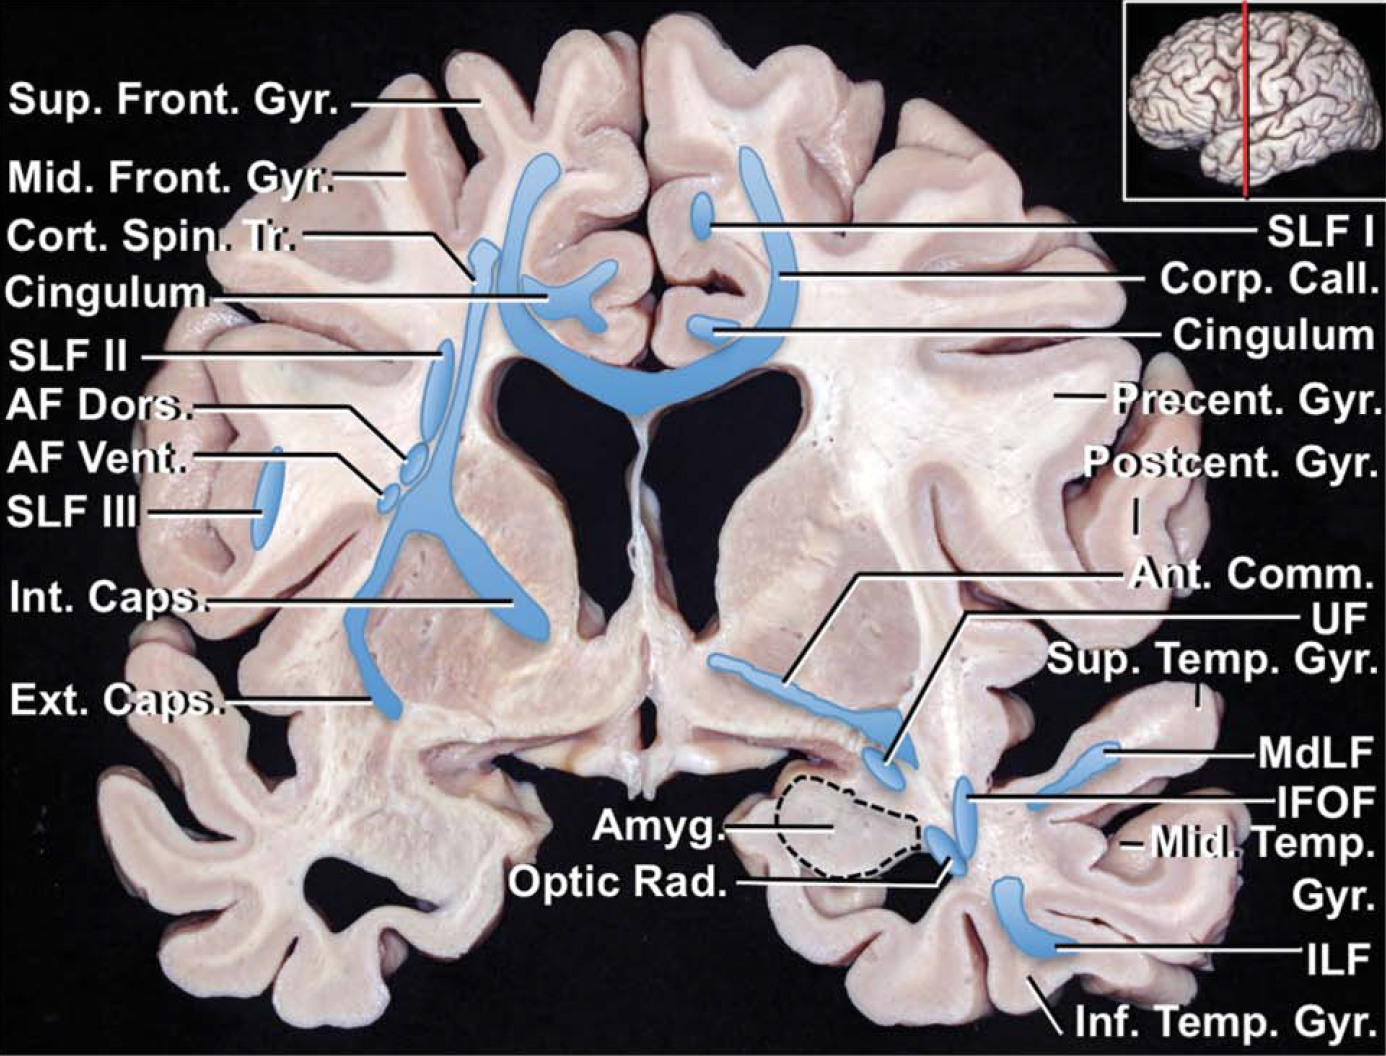
\includegraphics[width=0.6\linewidth, %angle=0]{figs/Anatomia_CST/anatomia_CST.png}
%    \legend{Fonte: \cite{yagmurlu2015}}
%    \caption{Localização de tratos em fatia coronal.}
%    \label{fig::CST_anatomia}
%\end{figure}

O CST é uma parte do trato piramidal e consiste no conjunto de fibras que se origina majoritariamente no córtex cerebral e segue em direção à medula espinhal \cite{Kolb2015}. Há forte evidência de que as fibras do CST estão relacionadas com o movimento de músculos esqueléticos voluntários \cite{zhang2018}.
A sua reconstrução \textit{in-vivo} é relevante tanto no que diz respeito a avaliação de lesões na medula espinhal, quanto em planejamento cirúrgico \cite{zhang2018}.

O que torna o CST interessante para o nosso estudo é, além de ser funcionalmente relevante, é um trato que atravessa todo o cérebro ascendentemente, cruzando ou tangenciando com uma série de fibras longitudinais e mediolaterais, como fascículo longitudinal superior (SLF), fascículo arqueado (AF) e corpo caloso (CC). Isso torna a sua reconstrução integral um desafio.



No experimento, as regiões de interesse (\textit{region of interest} - ROI) consistem em duas regiões que envolvem o pedúnculo cerebral, de acordo com o sugerido por \citeonline{DTI_Handbook}. A seleção, feita manualmente com a interface do VMTK-Neuro, é mostrada na figura \ref{fig::ROI}. As sementes para o processo iterativo de integração de linhas consistem em um subconjunto das ROIs que possuem um valor de FA alto (acima de 0,60).

\begin{figure}[ht]

%\subfigcapskip = -5pt
    \centering
    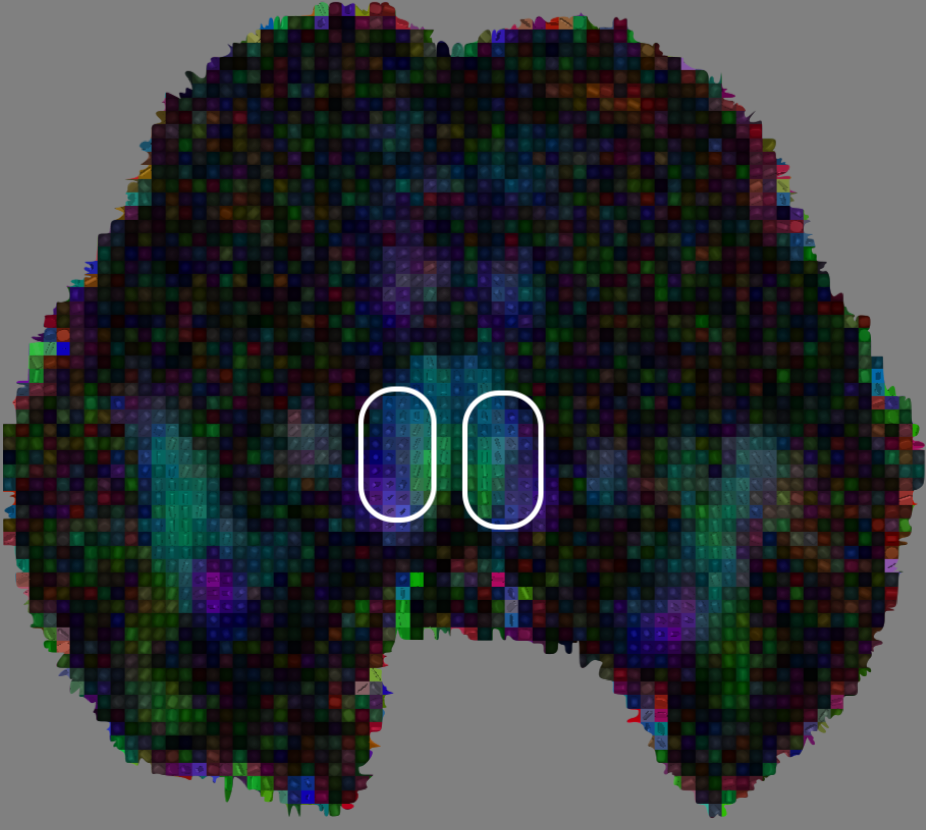
\includegraphics[width=.8\linewidth, angle=0]{figs/Tractografia/A27_SQ_3D.png}
    \caption{Mapa FA codificado por cores e glifos superquádricos. A ROI se situa dentro dos contornos de cor branca, no pedúnculo cerebral que possuem direções de difusão dominante ascendente (cor ciano e azul).}
    \label{fig::ROI}
   \hspace{1pt}
\end{figure}



O resultado do processo de geração de linhas representativas dos tratos está mostrada na figuras \ref{fig::DTI_Fatia_Coronal_Trato} e \ref{fig::trato}. Nota-se que o processo de integração de linhas, em sua maioria, é interrompido ou desviado na região de cruzamento de fibras e não condizem com a anatomia conhecida. Algumas linhas seguiram a direção anteroposterior (trato SLF), outras seguiram a direção mediolateral (corpo caloso) e algumas poucas linhas continuaram a ser integradas na trajetória ascendente.

\begin{figure}[ht]

%\subfigcapskip = -5pt
    \centering
%    \caption{Projeção Coronal - Volume e trato reconstruídos.}
    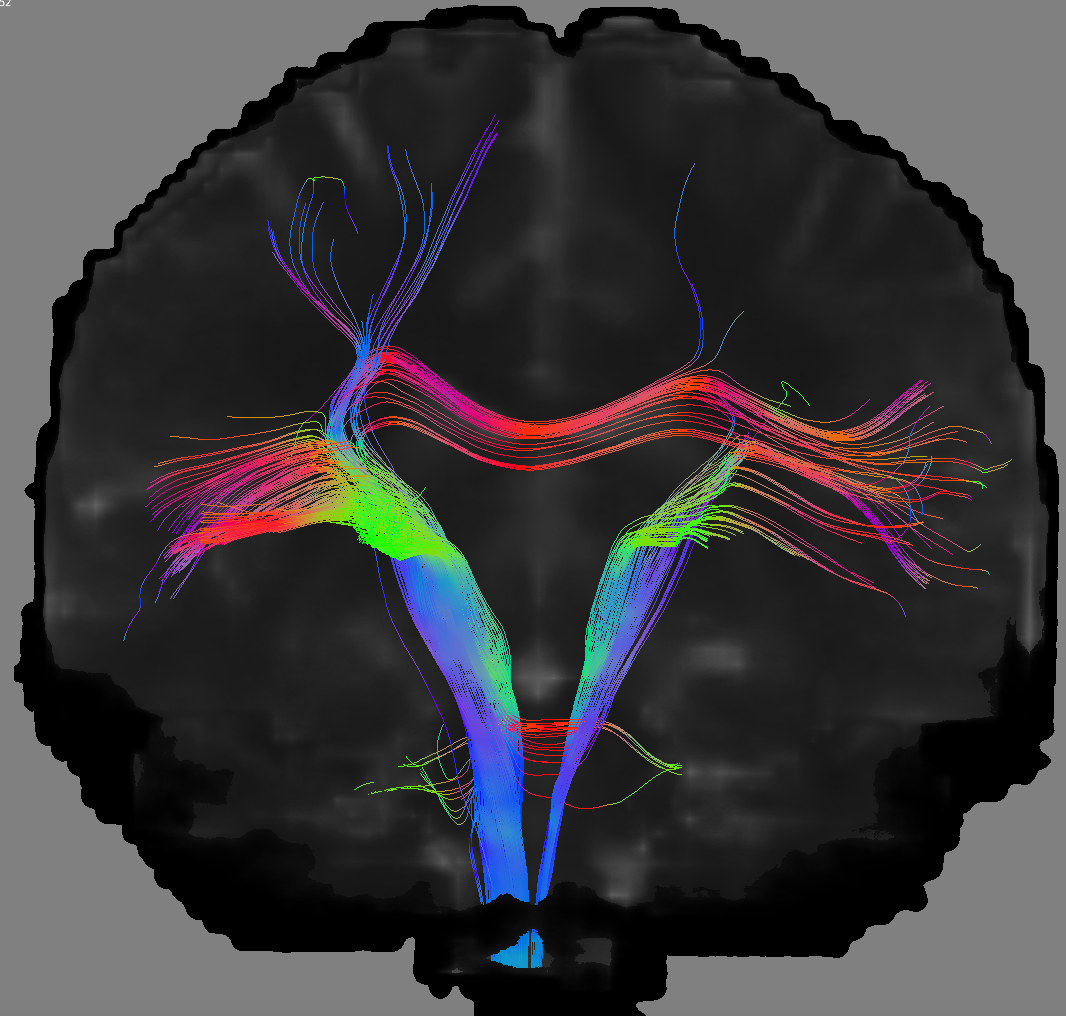
\includegraphics[width=.6\linewidth, angle=0]{figs/Tractografia/Trato_Volume.png}
        \caption{Fatia Coronal: fibras reconstruídas a partir das sementes no VMTK-Neuro.}
    \label{fig::DTI_Fatia_Coronal_Trato}
 %   \hspace{1pt}
\end{figure}

\begin{figure}[ht]
\captionsetup[subfloat]{farskip=0pt,nearskip=0pt}
    \subfloat[Axial.]{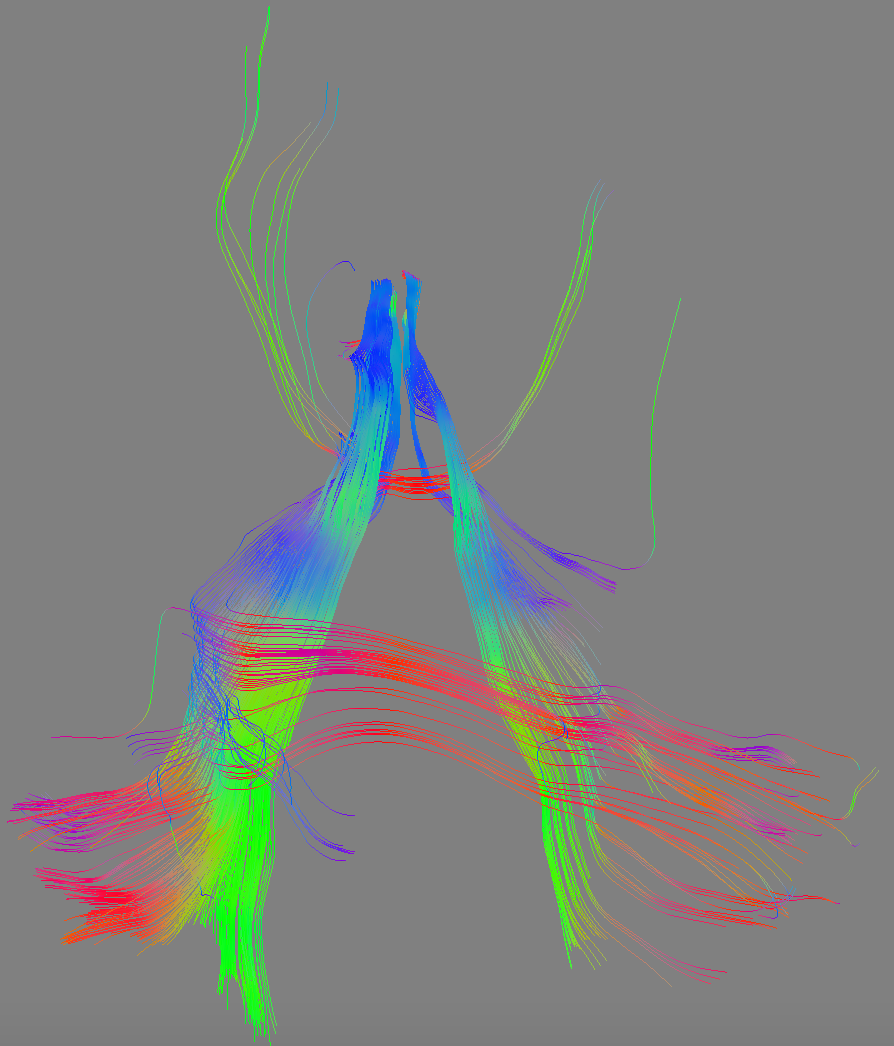
\includegraphics[width=.27\linewidth, angle=0]{figs/Tractografia/trato_axial.png}}
    \hfill
    \subfloat[Sagital.]{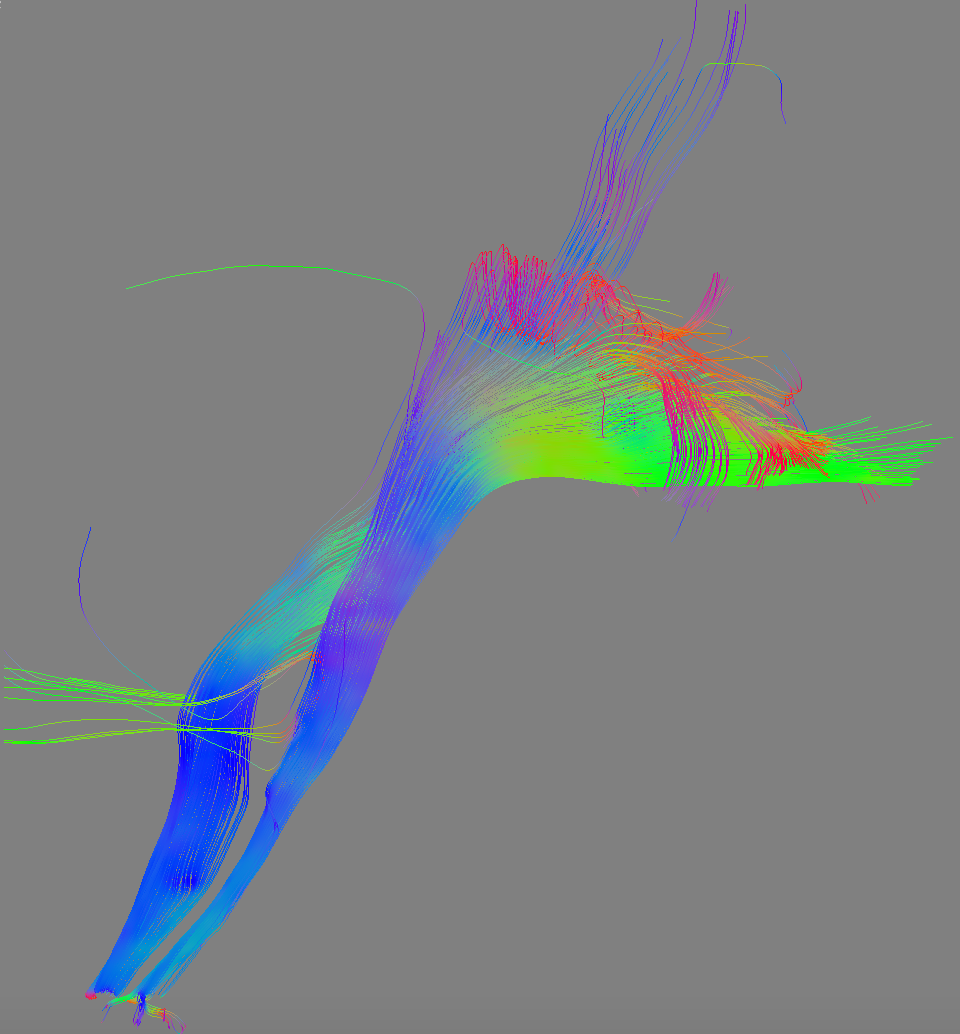
\includegraphics[width=.30\linewidth, angle=0]{figs/Tractografia/trato_sagital.png}}
    \hfill
    \subfloat[Coronal.]{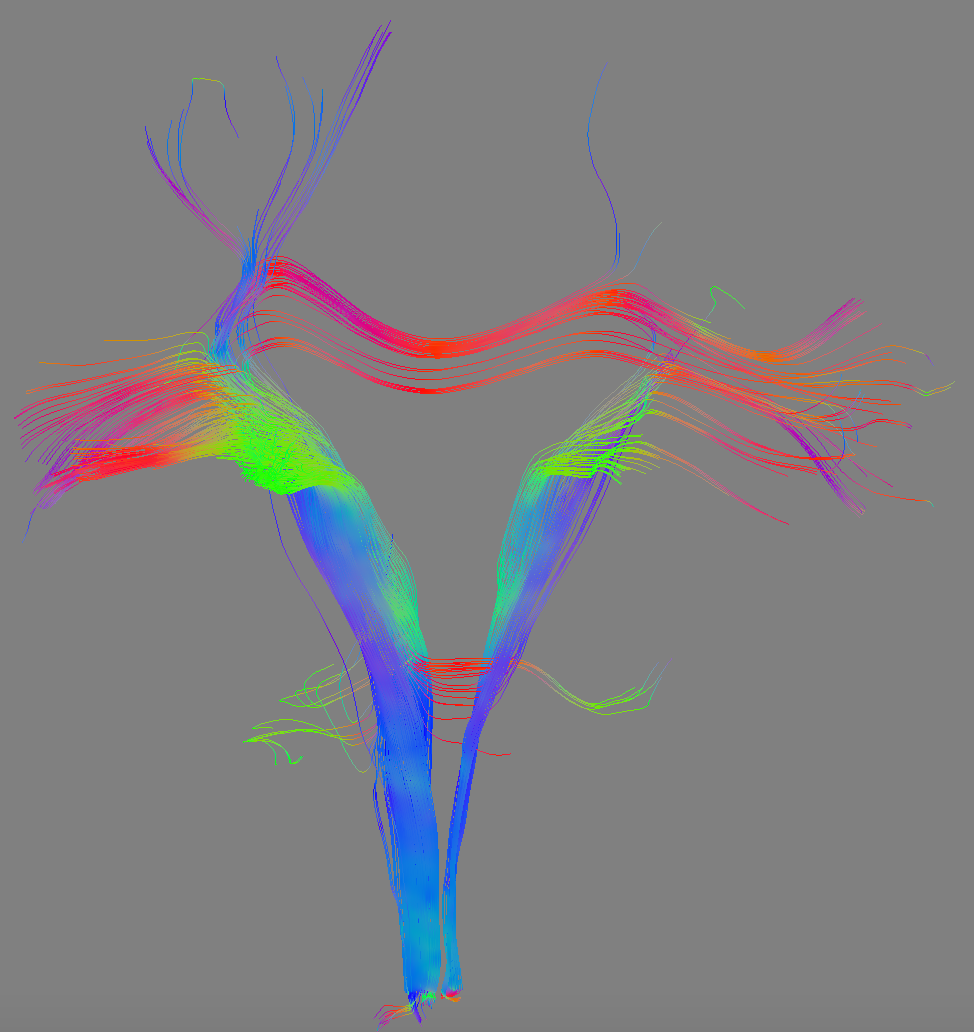
\includegraphics[width=.30\linewidth, angle=0]{figs/Tractografia/trato_coronal.png}}
     \caption{Linhas construídas sob diferentes ângulos.} %!!VER SE ISSO TA CERTO
    \label{fig::trato}
\end{figure}

O motivo que faz a maior parte das linhas não serem integradas na direção anatômica esperada se deve à forma como a decisão é tomada pelo algoritmo de tractografia no seu processo iterativo em cruzamento de fibras. Nesta situação, a integração de linhas é feita na direção associada ao maior autovalor do tensor de difusão, que não necessariamente é ascendente.

A figura \ref{fig::FA_coronal_Linhas1DTI} exemplifica o que ocorre na integração de linhas em uma região de cruzamento de fibras. Para nos situar, o processo de integração de linhas vem de sementes que estão na parte inferior da fatia e seguem na direção ascendente por regiões que tem esta direção de difusão principal. Nas regiões destacadas da fatia, que são de cruzamento de fibras e fazem parte do processo de integração de linhas, observa-se que a direção de difusão dominante não é ascendente.

O fato da direção dominante não ser ascendente resulta em dois tipos de decisão tomadas no processo iterativo: a integração das linhas ocorre na região mediolateral (evidenciado na figura \ref{fig::FA_coronal_Linhas1DTI}) ou anteroposterior, ou há a interrupção pelo critério de variação abrupta de ângulos ou baixo FA.

\begin{figure}[ht]
\centering
\captionsetup[subfloat]{farskip=5pt,nearskip=0pt}



\subfloat[Fatia coronal com cruzamento de fibras.] {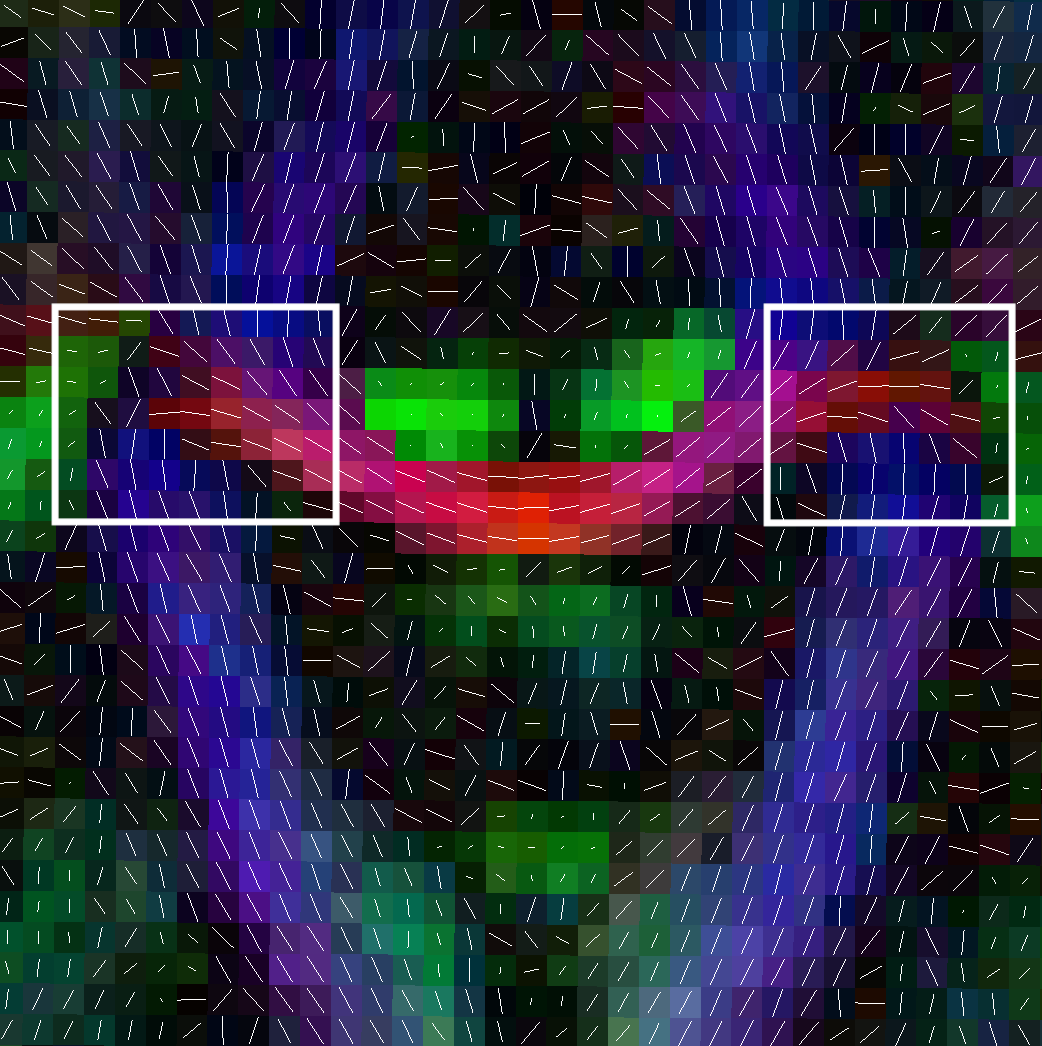
\includegraphics[width=.6\linewidth, angle=0]{figs/Tractografia/FA_coronal_Linhas1DTI.png}}    
    \linebreak
    \subfloat[Região de cruzamento de fibras a esquerda.]{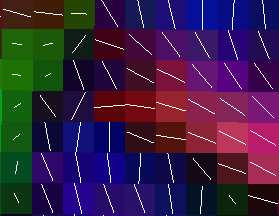
\includegraphics[width=.35\linewidth, angle=0]{figs/Tractografia/FA_coronal_Linhas1DTI_zoom.png}}
    \hfill
    \subfloat[Região de cruzamento de fibras a direita.]{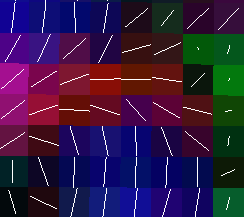
\includegraphics[width=.3\linewidth, angle=0]{figs/Tractografia/FA_coronal_Linhas1DTI_zoom2.png}}
    \caption{Direções de difusão associadas ao maior autovalor do tensor estimados em cada \textit{voxel} sobre um Mapa FA codificado por cor.}
    %\hfill
    \label{fig::FA_coronal_Linhas1DTI}
\end{figure}

%\textcolor{blue}{O fato de considerar ao longo de uma integração linear somente os autovetores de maior autovalor em cada amostra, o procedimento pode falhar nas amostras onde não há direções principais dominentes, como ilistra a Figura \ref{fig:comp_autovetor}. Observe na região destacada de cruzamento entre o trato corticoespinhal e o corpo caloso a perda de dados referentes à direção do trato corticoespinhal na Figura \ref{fig:comp_autovetor}.(a), detectada como segunda direção principal na Figura \ref{fig:comp_autovetor}.(b).}





%!!Colocar trato fatia coronal



%O resultado do processo de geração de linhas representativas dos tratos \textcolor{blue}{numa fatia coronal} está \sout{representada}\textcolor{blue}{mostrada} na figura \ref{fig::DTI_Fatia_Coronal_Trato}\sout{, acompanhado de uma fatia coronal e na}\textcolor{blue}{. A} figura \ref{fig::trato}\sout{, que} mostra o \textcolor{blue}{o mesmo } trato em diferentes projeções. É possível perceber que no processo iterativo para geração das linhas, o comportamento da reconstrução não é o esperado na região de cruzamento das fibras com o corpo caloso. O processo de integração das linhas acontece\sout{ram}\textcolor{blue}{u} de duas formas diferentes para as sementes das linhas abaixo e acima do corpo caloso.






%!!com o corpo caloso\sout{, para parte das linhas, um critério de parada é acionado e para outra, ela segue em direção ao corpo caloso}\textcolor{blue}{algumas linhas seguiram em direção do corpo caloso e outras interromperam o precurso por terem satisfeitas o critério de parada}.

%\todo[inline]{Reformular a segunda parte do parágrafo.}
%A região acima do corpo caloso gerou linhas que \todo{não necessariamente parte do limite superior!} partem do limite superior do cérebro e no momento da chegada no cruzamento de fibras, uma boa parte seguiu na direção do trato do corpo caloso e segue na direção da outra parte do trato bifurcado e uma parte menor seguiu na direção descendente.

%Na integração das linhas geradas a partir das sementes da direita, na passagem pela região de cruzamento de fibras na altura do corpo caloso, houveram desvios de algumas linhas para outras direções, além de uma interrupção das iterações, que acontece pelo critério de baixa anisotropia, ou por mudança brusca de direção da direção principal de maior difusão do tensor.
%Na integração das linhas geradas a partir das sementes da esquerda, há um claro desvio de caminho para a região do corpo caloso, onde as fibras terminam no limite do volume. Além disso, há uma quantidade menor de fibras seguem o caminho do trato CS.

%\todo[inline]{Figura 9 ficou solta ... }
%Observa-se também que há uma expansão das linhas para na parte abaixo das sementes iniciais em direção !!COMENTAR AS LINHAS VERDES DE BAIXO

%\begin{figure}[H]
%
%%\subfigcapskip = -5pt
%    \centering
%    \caption{Projeção Coronal - Volume de %difusão e trato reconstruído}
%    \includegraphics[width=.7\linewidth, %angle=0]{figs/Tractografia/Trato_DTI_Volume%_Coronal.png}
%    \label{fig::trato_DTI_Volume_Coronal}
% %   \hspace{1pt}
%\end{figure}

%\begin{figure}[H]

%%\subfigcapskip = -5pt
%    \centering
%    \caption{Projeção Coronal - Mapa de FA %codificado por cor,  e linhas %correspondentes à direção principal do %tensor de difusão.}
%    \includegraphics[width=.7\linewidth, %angle=0]{figs/Tractografia/Trato_DTI_Volume%_Linhas_Coronal.png}
%    \label{fig::Trato_DTI_Volume_Linhas_Coronal%}
% %   \hspace{1pt}
%\end{figure}

%\begin{figure}[H]
%\subfigcapskip = -5pt
%\subfigbottomskip = 0pt
%    \caption{Resultado do algoritmo de %tractografia em 3 projeções. Sistema de %coordenada direita, anterior, superior %(RAS).} %!!VER SE ISSO TA CERTO
%    \subfloat[Projeção %axial]{\includegraphics[width=.32\linewi%dth, angle=0]{figs/Tractografia/trato_ax%ial.png}}
%    \hfill
%    \subfloat[Projeção %sagital]{\includegraphics[width=.32\line%width, angle=0]{figs/Tractografia/trato_%sagital.png}}
%    \hfill
%    \subfloat[Projeção %coronal]{\includegraphics[width=.31\line%width, angle=0]{figs/Tractografia/trato_%coronal.png}}
%    \label{fig::trato}
%\end{figure}

%Para entender melhor o por quê há esse desvio no processo iterativo na tractografia, a figura \ref{fig::Trato_DTI_MapaFA_Linhas} mostra uma fatia coronal de um mapa FA codificado por cor e com cada \textit{voxel} preenchido com pequenos segmentos de reta de cor branca na região de cruzamento do trato CS com o corpo caloso. Cada segmento representa a direção do autovetor associado a maior \textcolor{blue}{autovalor de} difusão extraído do tensor, direção esta que domina na estimativa da direção da linha em reconstrução em cada \textit{voxel} no processo de tractografia. Observa-se que na região de cruzamento do trato CS com o corpo caloso, a direção principal do tensor 
%é predominante na região do corpo caloso, o que induz que a fibra no seu processo de integração tenha \todo{Não está claro para mim a correspondência entre o desvio e as linhas brancas na figura. Sugestão: destacá-lo na figura.}esse desvio.

%\todo[inline]{Sugestão: destacar na Figura 10 as regiões onde ocorreram ``desvios''.}
A nossa conjectura levantada, como mencionado no capítulo \ref{proposta}, consiste em que, tendo acesso a orientações amostradas plausíveis e critérios apropriados para seleção da melhor orientação numa integração linear específica, o algoritmo de tractografia faz a integração de linhas na direção mais adequada para a fibra que está sendo reconstruída.


%\begin{figure}[ht]
%
%%\subfigcapskip = -5pt
%    \centering
%%    \caption{Projeção Coronal - Mapa de FA codificado por cor e %linhas correspondentes à direção principal do tensor de difusão. %%As sementes iniciais usadas para a tractografia estão contidas %nas regiões circulares de cor branca.
%%    }
%    \caption{!!desconectado Fatia coronal: mapa de FA codificado %por cor e linhas correspondentes à direção principal do %tensor de difusão. 
%    }
%    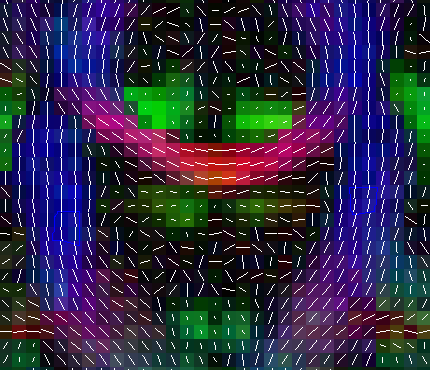
\includegraphics[width=0.8\linewidth, %angle=0]{figs/Tractografia/DTI_mapaFA_Linhas_Cruzamento.png}
%    \label{fig::Trato_DTI_MapaFA_Linhas}
% %   \hspace{1pt}
%\end{figure}

%\pagebreak

\section{\sout{Implementação do }\textit{Q-Ball}}

O \textit{QBall} foi implementado como o algoritmo proposto por \citeonline{TuchQBall2004}. O domínio $\{\textbf{u}\}$ foi retirado de uma malha esférica gerada a partir da discretização das coordenadas $(\theta, \phi)$. Um exemplo de malha esférica obtida com essa abordagem está ilustrado na figura \ref{fig::MalhaEsferico}.
A abordagem de implementação consiste no cômputo de todas as ODFs para cada \textit{voxel} do volume para posterior uso no algoritmo de extração de picos e geração de glifos.

%\todo[inline]{A sua proposta é aplicar o algoritmo de Tuch?}Foi implementado o algoritmo para estimação de ODF para volumes DWI de acordo com o proposto por \citeonline{TuchQBall2004}.

%\todo{Não é melhor tirar esta figura para não confundir?}%\sout{A figura \ref{fig::MalhaEsferico} mostra a abordagem.}
%No decorrer do trabalho, a malha esférica será substituída por um icosaedro tesselado. A vantagem dessa malha é que, olhando as direções na perspectiva de vértice de uma esfera, a distância entre vizinhos é a mesma para toda esfera. O conceito de proximidade entre esses vértices é importante na escolha de direções para tractografia.

%\begin{figure}[ht]
%
%%\subfigcapskip = -5pt
%    \centering
%    %\vspace*{1mm}
%    \includegraphics[width=0.5\linewidth, %angle=0]{figs/Exemplos_QBall_visualizacao/MeshEsfe%rico.png}
%        \caption{Malha Esférica - Ambos $\phi$ e %$\theta$ discretizados em 15 valores.}
%    \label{fig::MalhaEsferico}
% %   \hspace{1pt}
%\end{figure}

%\begin{figure}[H]
%
%%\subfigcapskip = -5pt
%    \centering
%    \caption{Malha Esférica - Múltiplas malhas %com icosaedro tesselado.}
%   % \vspace*{1mm}
%    \includegraphics[width=0.8\linewidth, %angle=0]{figs/Exemplos_QBall_visualizacao/I%cosahedronMesh.png}
%    \legend{Fonte: \cite{icosahedron2017}}
%    \label{fig::MalhaIcosaedro}
% %   \hspace{1pt}
%\end{figure}



%\subsection{Renderização de Glifos}

%\todo{A sua proposta é aplicar os glifos propostos por Tuch na visualização de ODFs?}

%\todo[inline]{Limites de tempos de resposta:
%\url{https://www.nngroup.com/articles/response-times-3-important-limits/}

%Foi implementado um esquema de visualização para ODFs em glifos de acordo com o proposto por \citeonline{TuchQBall2004}. A implementação serviu primeiramente para prova de conceito e posteriormente otimizada para que seja possível a sua renderização, \textit{voxel} a \textit{voxel}, em tempo interativo pelo VMTK-Neuro, o que foi possível nos testes feitos em um Macbook Pro Retina 13', com processador Intel Core i5 Dual-Core 2.7Ghz, processador gráfico Intel Iris Graphics 6100 1536 MB e memória RAM de 8 GB 1867 MHz DDR3.

%\citeonline{peeters2009} apresentou pela primeira vez um esquema de renderização para esta categoria de glifos, nos quais são aperfeiçoados por \citeonline{peeters2011} e \citeonline{hlawitschka2012}, utilizando \textit{raycasting}!!(VER OS ARTIGOS). No VMTK-Neuro, um dos algoritmos de renderização do tensor difusão por superquádricas é feita por instanciação de malhas esféricas, que são modificadas por parâmetros particulares a cada tensor de difusão referentes a cada voxel detectado, e posicionado na cena de acordo. O esquema de renderização ocorre em tempo interativo, e tem performances, que foram medidas pelo nosso grupo de pesquisa, comparáveis aos algoritmos baseados em \textit{raycasting} da mesma categoria !!\ref{}.

%Pela maior simplicidade e boa efetividade da renderização pelas instanciações de uma malha esférica, onde o glifo é modificado por parâmetros particulares de cada perfil de difusão e que tem sido previamente implementado na renderização de glifos superquádricos, o esquema desenvolvido para representação polar esférica utiliza uma adaptação desta abordagem.

%No que diz respeito ao posicionamento dos glifos em fatias e na renderização tridimensional, foi utilizada toda a infraestrutura já existente no VMTK-Neuro para este fim que atualmente suporta a representação do tensor de difusão por superquádricos. \citeonline{raphael_dissertacao} detalha o processo de detecção de \textit{voxels} em um volume tridimensional e \textit{pixels} em fatias e o posicionamento associado em sua dissertação de mestrado. 

%Dados relativos ao desempenho \sout{serão mais detalhados na dissertação de mestrado}\textcolor{blue}{estão disponíveis no link ...}.

%No apêndice, na subseção \ref{section::QBall_Glifos}, seguem algumas imagens dos glifos derivados das ODFs implementado no VMTK-Neuro. O volume é derivado da competição ISMRM \cite{TractometerTool}. A malha esférica utilizada é a mesma da figura \ref{fig::MalhaEsferico}.

%\sout{Medições do tempo relativo ao desempenho foram feitas para a quantidade de 197 vértices da malha esférica \sout{em um}\textcolor{blue}{num} volume de resolução 128x128x90. Para uma quantidade na faixa de 5000 glifos renderizados simultaneamente sobre uma fatia completa, obtemos tem um tempo de resposta entre 80 e 110ms. Para uma quantidade pequena de glifos na faixa das dezenas, o tempo de resposta cai para o intervalo entre 60 e 70ms. Esse tempo de resposta está nas proximidades ou é menor do que o tempo de 0,1s, que é o limite máximo para que o usuário tenha a percepção de resposta instantânea da máquina e que suas ações são a causa de que algo aconteça na tela \cite{nielsen1994}.}

%\sout{No cômputo das ODFs do \textit{QBall}, é feito o mapeamento do sinal de DWI para a ODF a partir das direções derivadas da malha esférica. O glifo para visualização é gerado diretamente de acordo a representação gráfica polar esférica em que $R(\textbf{u}) = \psi(\mathbf{u})$, onde \textbf{u} é a direção de difusão. A malha esférica utilizada para geração dos glifos em \ref{section::QBall_Glifos} está representada na figura \ref{fig::MalhaEsferico}.}

%A priori, todas as ODFs são calculadas e normalizadas para o intervalo $[0,1]$ para cada um dos \textit{voxels} do volume e referenciadas no processo de renderização.

%O formato de armazenamento dos valores ODF associados à malha consiste numa lista de valores escalares associados a cada um dos \textit{voxels}.



%\todo[inline]{Falta uma descrição melhor de como são construídos os glifos a partir de ODFs e o seu mapeamento às entidades gráficas. Isso torna difícil o entendimento da sua implementação. !!Descrito em trabalhos relacionados!}

%A abordagem utilizada para renderização consiste em instanciações de uma malha esférica centrada na origem, raio unitário e sem repetição de pontos. A cada instância, a malha é transformada por duas classes de elementos: os elementos em comum a todos os \textit{voxels} e os particulares.

%Os elementos comuns se referem às transformações de escala e às transformações referentes à orientação. O fator de escala, que é função do \textit{zoom} aplicado e dimensão do \textit{voxel}, bem como o cômputo das transformações relativas à orientação, que se referem aos sistemas de orientação neurológica (LAS) e radiológica (RAS) que já constavam no VMTK-Neuro e foram adaptados para implementação em questão.% e sincronização com fatias bidimensionais.


%Há dois elementos particulares que customizam os glifos, cujos dados são enviados à GPU a cada \textit{frame} após os \textit{voxels} aparentes na cena serem detectados. O primeiro é a translação para reposicionamento, que desloca a malha para o centro do seu respectivo \textit{voxel} e o segundo diz respeito às ODFs particulares a cada \textit{voxel}, que determina a forma do glifo através da multiplicação do vértice da malha associada à direção de difusão ao seu valor de ODF. 



%O problema no valor de ODFs é que não há parâmetros em comum entre vértices da mesma esfera instanciada. A API OpenGL e a linguagem GLSL não oferecem formas diretas de se fazer alocação dinâmica de memória na GPU, em que disponibilize N*M valores de ODF para N \textit{voxels} aparentes na tela e uma malha esférica de M vértices.

%\todo[inline]{Como foi a estruturação na textura? Procurou explorar a coalescência/a sequência de acessos?}


%A estratégia adotada para superar esse problema foi o  armazenamento dos dados de ODF dos \textit{voxels} detectados e o envio para GPU como uma textura 2D, onde é possível acessar os dados de ODF de acordo com índices de instância (relativo ao \textit{voxel}) e o índice de vértice (relativo à malha esférica instanciada na GPU). %Evidentemente que há um mapeamento do domínio $[0,1]^2$, que é padrão numa unidade de textura, para a quantidade de instâncias e vértices que são processados.

%As cores dos glifos consistem são um mapeamento direto do valor absoluto dos vértices $(x_v,y_v,z_v)$ da malha esférica para as suas componentes RGB, conforme mostrado na equação \ref{eq::cor_glifo}. Essa forma de mapear, além de simples, entra muito em acordo com a codificação em cores definidos no mapa de FA e faz o entendimento do glifo ser intuitivo. Não foi implementado o cômputo de vetores normais à superfície representadas pelo glifo, que consequentemente não tem iluminação associada.

%\begin{equation}
%\label{eq::cor_glifo}
%    (r,g,b) = (|x_v|,|y_v|,|z_v|)
%\end{equation}

%Medições do tempo relativo ao desempenho foram feitas para a quantidade de 197 vértices da malha esférica num volume de resolução 128x128x90. Para uma quantidade na faixa de 5000 glifos renderizados simultaneamente sobre uma fatia completa, obtemos tem um tempo de resposta entre 80 e 110ms. Para uma quantidade pequena de glifos na faixa das dezenas, o tempo de resposta cai para o intervalo entre 60 e 70ms. Esse tempo de resposta está nas proximidades ou é menor do que o tempo de 0,1s, que é o limite máximo para que o usuário tenha a percepção de resposta instantânea da máquina e que suas ações são a causa de que algo aconteça na tela \cite{nielsen1994}.

%A comparação de performance e alocação de memória com outras técnicas utilizadas irão constar na monografia de mestrado.

%\todo[inline]{Não é melhor "Extração de Direções Plausíveis"?}

\subsection{Extração de Direções Plausíveis}
%\subsection{Extração de picos}
\label{ExtracaoDirecoes}

%\todo{Qual é a sua proposta para extração de picos?}No momento, estão sendo implementados algoritmos que fazem a extração de múltiplas direções para serem utilizadas para a tractografia a partir da ODF.

Como mencionado em \ref{QBall_para_tractografia}, a informação extraída das ODFs utilizadas em tractografia são as métricas de anisotropia e informações relacionadas a direções.

Foi implementado o cômputo do GFA e a extração de picos proposta por \citeonline{descoteaux2007}. O cômputo do GFA foi implementado de acordo com a equação \ref{eq::gfa}. A extração de picos consiste na identificação de máximos locais das funções esféricas e a aplicação de um \textit{threshold} para retirar picos espúrios que eventualmente sejam detectados nos \textit{voxels}.

Foi também implementado um esquema de renderização para visualização de picos, que consiste no desenho de linhas brancas em seus respectivos \textit{voxels} em suas respectivas direções, que servirão de prova de conceito.

%\todo[inline]{O que adicionei abaixo pode ilustrar melhor o quê você está buscando e por quê, embora seja um fato aceito pela comunidade ... como trabalho de mestrado é interessante que você tenha este feeling prático ...}

A figura \ref{fig::Trato_QBall_MapaFA_Linhas} mostra os picos de ODF \textit{voxel} a \textit{voxel} na mesma fatia da figura \ref{fig::FA_coronal_Linhas1DTI}. A parte destacada mostra que os picos detectados na região de cruzamentos de fibra representam direções plausíveis dos três tratos (SLF, CST e corpo caloso) e mostram o potencial de uma tractografia feita a partir desta abordagem.

%\begin{figure}[h]
%
%\subfigcapskip = -5pt
%    \centering
%%    \caption{Projeção Coronal - Mapa FA codificado por cores e %picos extraídos as ODFs}
%   \caption{Mapa FA codificado por cores e picos extraídos das %ODFs em uma fatia coronal no cruzamento do corpo caloso.}
%   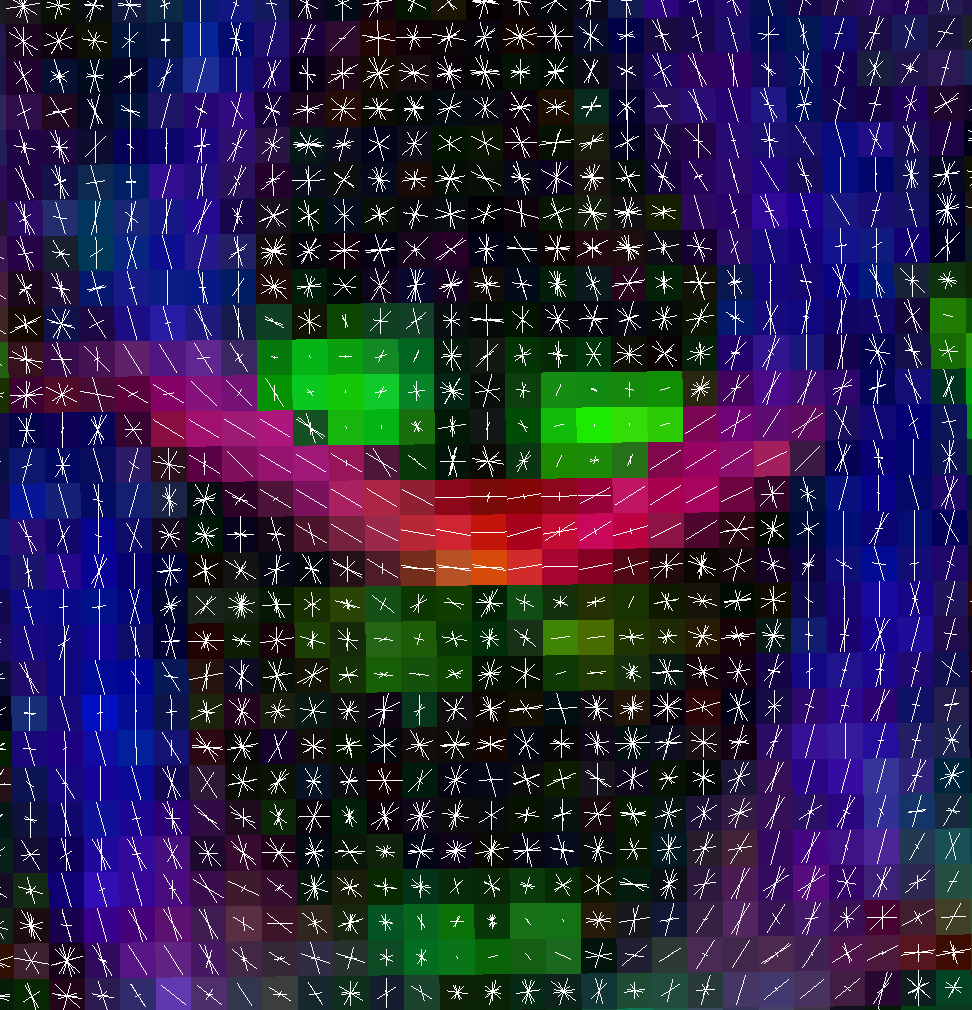
\includegraphics[width=.8\linewidth, %angle=0]{figs/Tractografia/MapaFA_Linhas_ROI.png}
%    \label{fig::Trato_QBall_MapaFA_Linhas}
% %   \hspace{1pt}
%\end{figure}

\begin{figure}[ht]
\centering
\captionsetup[subfloat]{farskip=5pt,nearskip=0pt}
%    \caption{Amostra do cruzamento de fibras entre corpo caloso, trato corticospinhal e fascículo longitudinal superior.} %!!VER SE ISSO TA CERTO
\subfloat[Mapa FA codificado por cores e picos de ODF.] {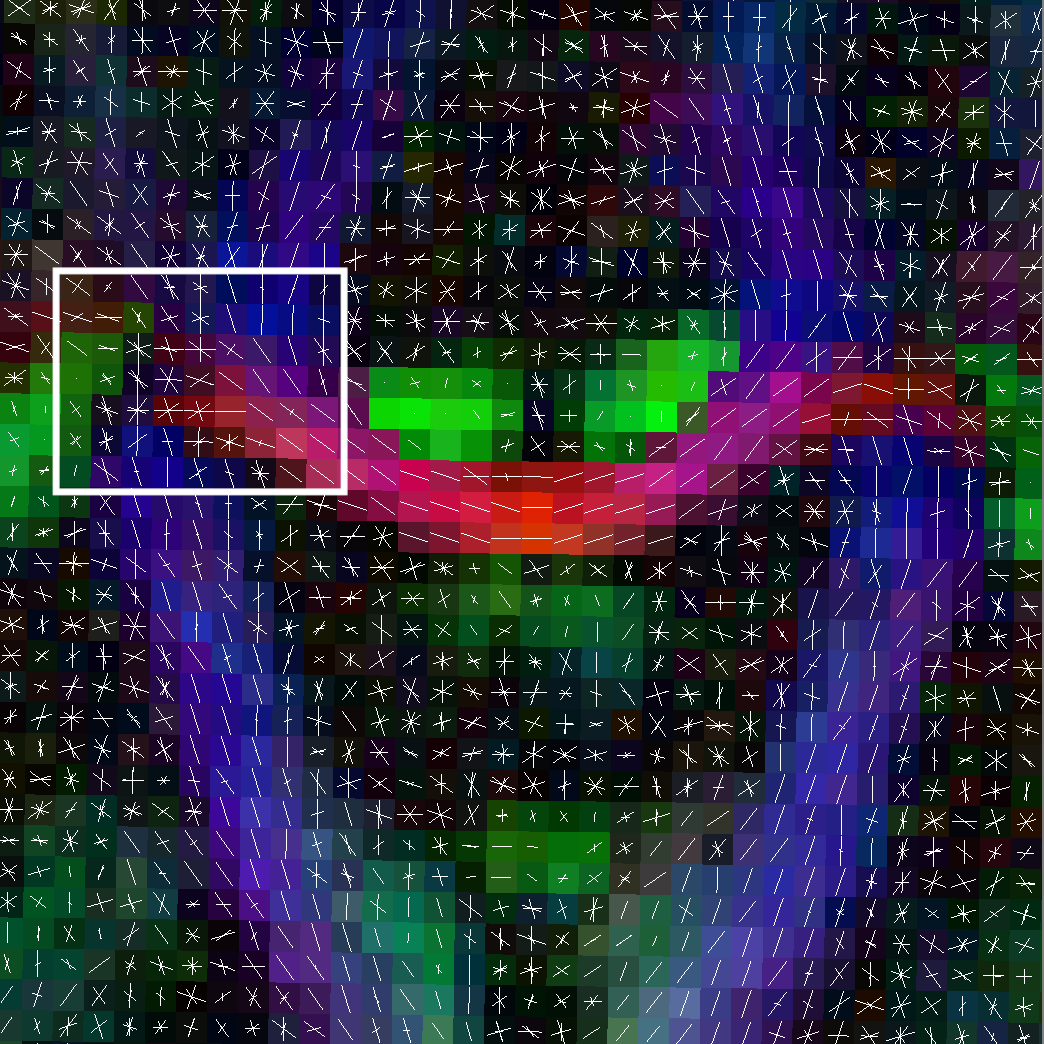
\includegraphics[width=.7\linewidth, angle=0]{figs/Tractografia/FA_coronal.png}}    
    \hfill
    \subfloat[Região de cruzamento de fibras.]{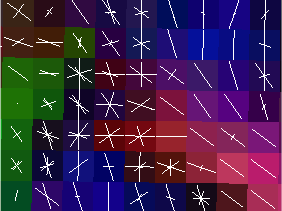
\includegraphics[width=.4\linewidth, angle=0]{figs/Tractografia/FA_coronal_zoom.png}}
    \caption{Amostras de difusão representadas pelas direções plausíveis (picos) extraídas das ODFs no cruzamento de fibras do corpo caloso, do trato corticoespinhal e do fascículo longitudinal superior.}    
    %\hfill
    \label{fig::Trato_QBall_MapaFA_Linhas}
\end{figure}



%que consiste \ref{fig::Trato_DTI_MapaFA_Linhas} no experimento de tractografia para DTI, está na figura \ref{fig::Trato_QBall_MapaFA_Linhas}. O valor de \textit{threshold} utilizado é metade do máximo absoluto da ODF.


%Comparando as figuras \ref{fig::Trato_DTI_MapaFA_Linhas} e \ref{fig::Trato_QBall_MapaFA_Linhas}, e analisando o percurso das linhas na direção ascendente podemos observar dois comportamentos para as direções dos \textit{voxels} de cor predominantemente azul, que tem direção dominante de difusão ascendente.

%A primeira é que, em ambas figuras, ao analisar linhas dos \textit{voxels} azuis de forma descendente a partir das regiões na parte superior da imagem, há uma parte que segue na direção do trato do corpo caloso, que estão mais próximas do centro da figura e outra parte minoritária que continua na direção descendente.

%\todo[inline]{Reformule o parágrafo. Está difícil para entender ...}
%A segunda, ocorre quando seguindo as linhas dos \textit{voxels} azuis partindo da parte inferior da fatia é  observável que na figura \ref{fig::Trato_QBall_MapaFA_Linhas}, na região do cruzamento com o corpo caloso, em que está representado por um tom vermelho e magenta escuro, há linhas brancas em uma direção ascendente e inclinadas se cruzando com retas que convergem para o trato do corpo caloso. Na figura \ref{fig::Trato_DTI_MapaFA_Linhas}, há um término abrupto das direções ascendentes, que por sua vez passam a convergir para o corpo caloso e que, no algoritmo baseado em DTI, pode haver a interrupção das iterações da tractografia.

%]\todo[inline]{Sugiro que você destaque nas imagens os pontos que você quer chamara atenção. Isso ajuda o leitor seguir o seu raciocínio.}
%A partir desta imagem, a conjectura da tractografia baseada em \textit{QBall} do trato CS tem potencial de gerar bons resultados para sementes iniciais localizadas abaixo do corpo caloso, por gerar linhas e direções dominantes que entram em concordância do esperado no cruzamento das duas fibras, podendo seguir em direção ascendente nas iterações do algoritmo.

%\textcolor{blue}{As regiões onde ocorreram desvios indevidos na expansão das fibras são destacadas nas figuras (a serem adicionadas). Chamamos atenção para o fato de que há direções que correspondem às de CS quase igualmente prováveis às de corpo caloso, enquanto no modelo de tensores de difusão os outros dois autovetores, secundários e terciários, nem sempre revelam esta diferença de forma tão explícita.}



%\subsection{Resultados com Volumes do HC}

%\todo[inline]{Uma breve descrição dos problemas que você detectou ao aplicar o seu algoritmo em volumes de HC e a descoberta da causa do problema ... A confirmação com novo protocolo de aquisição (a ser feita ainda).}

%\section{Testes com GQI}

%\todo[inline]{Sugiro que façamos os primeiros testes com DSI aplicando GDI para ver se temos algum insight mais interessante.}
\subsection{Tractografia}

\chapter{Futuros trabalhos}

Na renderização de glifos, pode-se implementar o cômputo de vetores normais para serem usados na iluminação das superfícies, o que é algo comum na apresentação por glifos. Adicionalmente, podemos implementar as representações polares esféricas sugerida por \citeonline{hlawitschka2012} e/ou \citeonline{peeters2011} para fins de comparação de performance com a nossa abordagem.

Em tractografia, o próximo passo é a implementação do afiamento de ODFs, o que melhora extração de direções plausíveis de direções a serem usadas no \textit{tracking} de fibras \cite{fillard2011, SCHILLING2019194}.



\chapter{Conclusões}

Neste trabalho foi abordamos a visualização de volumes DWI pelo método de imageamento para difusão Q-Ball, com o objetivo de integrá-lo ao ambiente multimodal em desenvolvimento pelo nosso grupo de pesquisa \cite{VMTKNeuro}, bem como desenvolver aplicações de visualização associadas. Adaptando muito do que já fora desenvolvido para o DTI, as aplicações desenvolvidas para o método consistem na estimação de ODFs via transformada de Funk-Radon, visualização em tempo interativo de ODFs em glifos e o desenvolvimento de um algoritmo de tractografia associado.

Objetivando prover um ambiente que permite a avaliação de ODFs, aproveitando as funcionalidades presentes no VMTK-Neuro para exploração de DWIs e MRI anatômicos, foi desenvolvido um esquema de renderização em tempo interativo que mapeia as ODFs em suas representações gráficas polares esféricas.

Com o objetivo de melhorar e tractografia baseada em DTI, foi implementado um protótipo de algoritmo de tractografia baseado em um conjunto de direções de métodos HARDI. !!(No trato corticoespinhal, no qual o DTI não consegue resolver).
Adicionalmente, a tractografia gera resultados em tempo interativo para o usuário, permitindo-o explorar livremente para diferentes parâmetros.

\pagebreak
\chapter{Apêndice}


\section{Imagens de ODFs mapeadas em glifos renderizadas no VMTK-Neuro}

\label{section::QBall_Glifos}

\begin{figure}[H]
\label{fig::QBall_glifos_axial}
%\subfigcapskip = -5pt
    \centering
    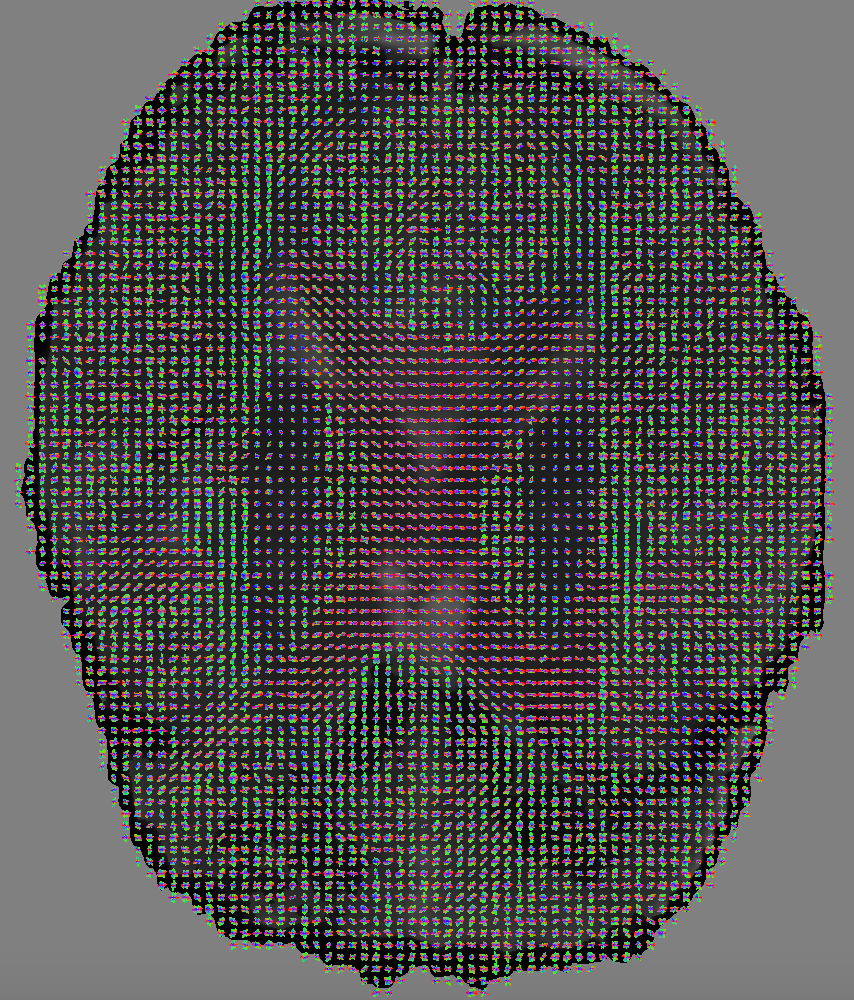
\includegraphics[width=1.0\linewidth, angle=0]{figs/Exemplos_QBall_visualizacao/Axial.png}
     \caption{Projeção Axial.}
 %   \hspace{1pt}
\end{figure}

\begin{figure}[H]
\label{fig::QBall_glifos_sagital}
%\subfigcapskip = -5pt
    \centering

    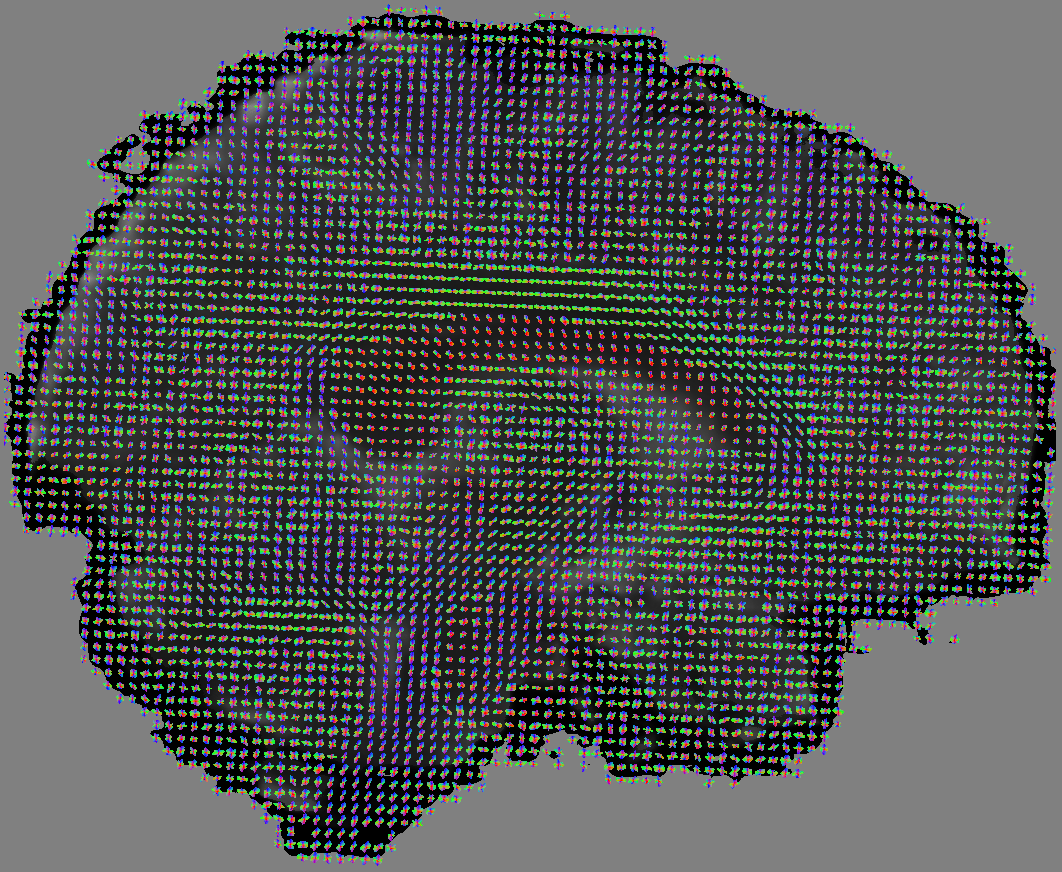
\includegraphics[width=.7\linewidth, angle=0]{figs/Exemplos_QBall_visualizacao/Sagital.png}
    \caption{Projeção Sagital.}
 %   \hspace{1pt}
\end{figure}

\begin{figure}[H]
\label{fig::QBall_glifos_coronal}
%\subfigcapskip = -5pt
    \centering

    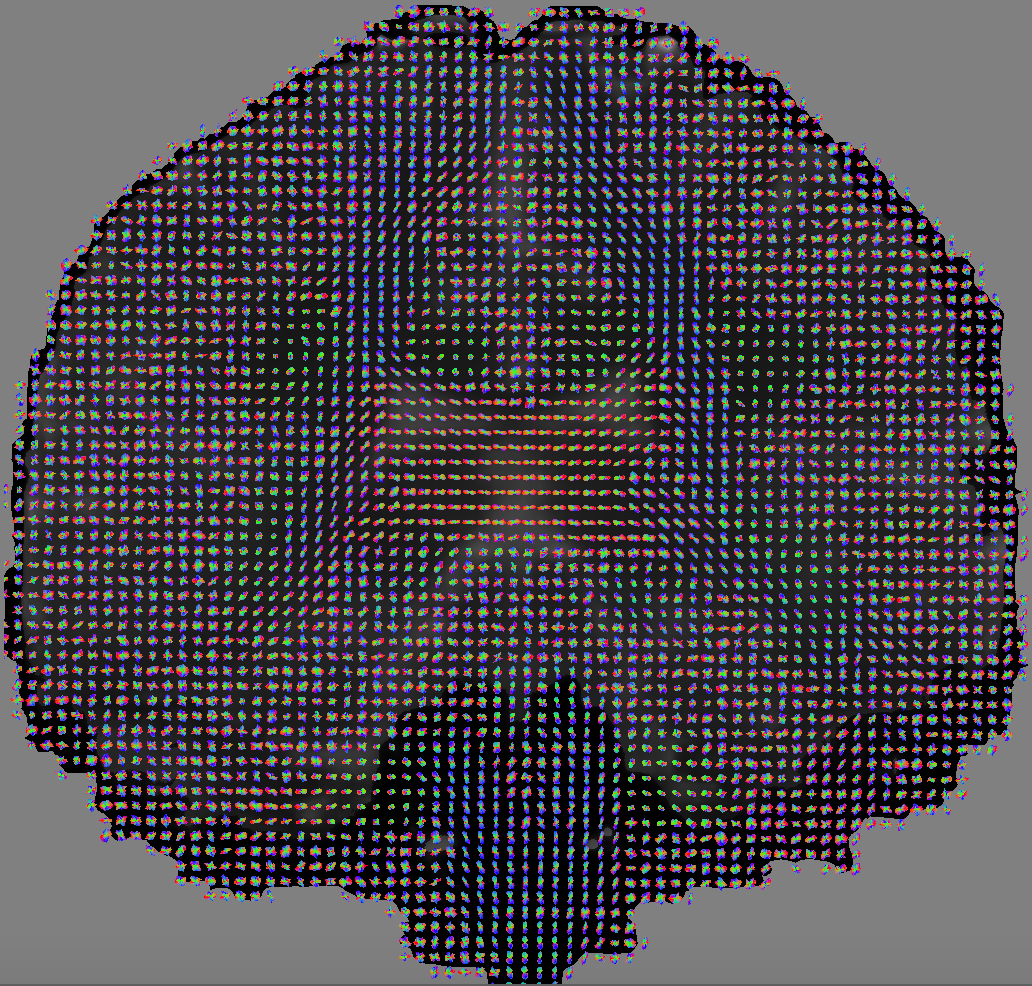
\includegraphics[width=0.7\linewidth, angle=0]{figs/Exemplos_QBall_visualizacao/Coronal.png}
    \caption{Projeção Coronal.}
 %   \hspace{1pt}
\end{figure}

\begin{figure}[H]
\label{fig::QBall_glifos_Coronal_CC_CS}
%\subfigcapskip = -5pt
    \centering
    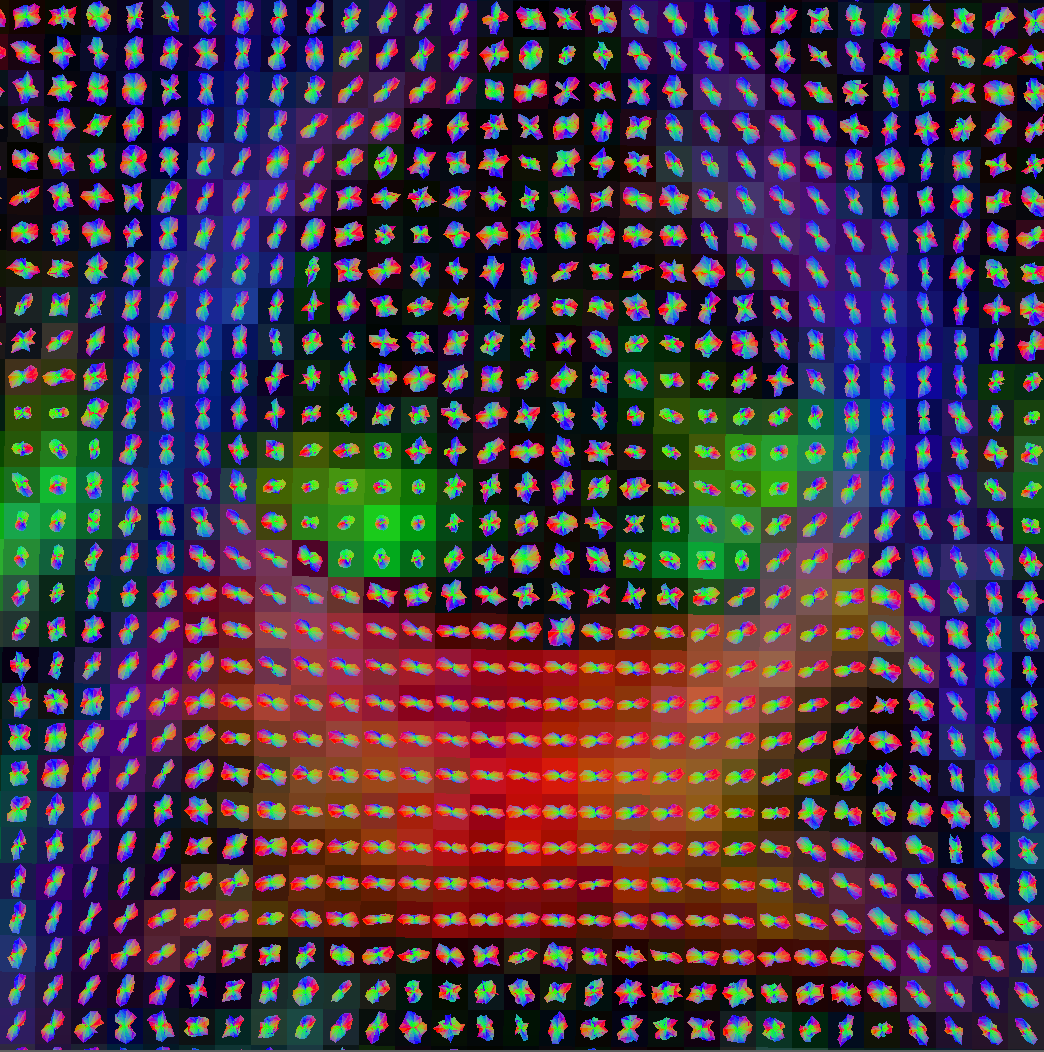
\includegraphics[width=.7\linewidth, angle=0]{figs/Exemplos_QBall_visualizacao/Coronal_Cruzamento_MapaFA.png}
    \caption{Projeção Coronal - Região de cruzamento de fibras. Glifos renderizado sobre mapa FA codificado por cores do DTI.}
 %   \hspace{1pt}
\end{figure}

\begin{figure}[H]
\label{fig::QBall_glifos_azul}
%\subfigcapskip = -5pt
    \centering

    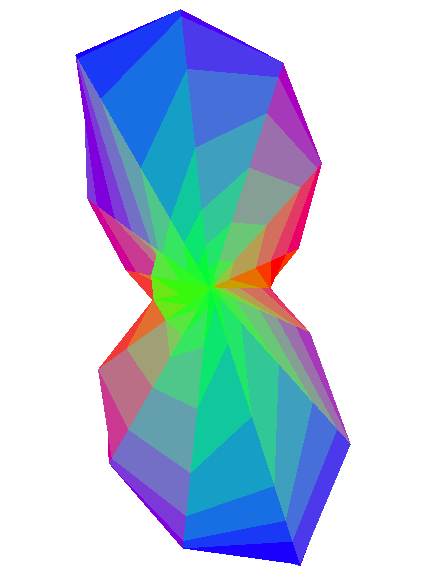
\includegraphics[width=.4\linewidth, angle=0]{figs/Exemplos_QBall_visualizacao/Glifo_Azul.png}
    \caption{Glifo referente a um voxel com direção de difusão predominantemente ascendente.}
 %   \hspace{1pt}
\end{figure}

\pagebreak


\section{\textit{Overplus} e problemas com o mapeamento do sinal de difusão em ODFs}
\label{ssec::problema_overplus}

Após um estudo que visou comparar ODFs geradas a partir de diferentes esquemas de amostragem de gradientes de ponderação de difusão, concluímos que a falta de uniformidade do conjunto de gradientes do \textit{Overplus} no domínio esférico compromete a interpolação de sinais de difusão no processo de cômputo do \textit{Q-Ball}. A figura \ref{fig::shell_Overplus_VS_ISMRM} mostra a distribuição no \textit{shell}\footnote{\textit{Shell} é um consiste em um conjunto definido em uma esfera.} das direções dos gradientes do \textit{Overplus}, em adição ao utilizado no volume ISMRM 2015.

\begin{figure}[ht]
\centering
\captionsetup[subfloat]{farskip=5pt,nearskip=0pt}
    %!!VER SE ISSO TA CERTO
    \subfloat[\textit{Overplus}.] {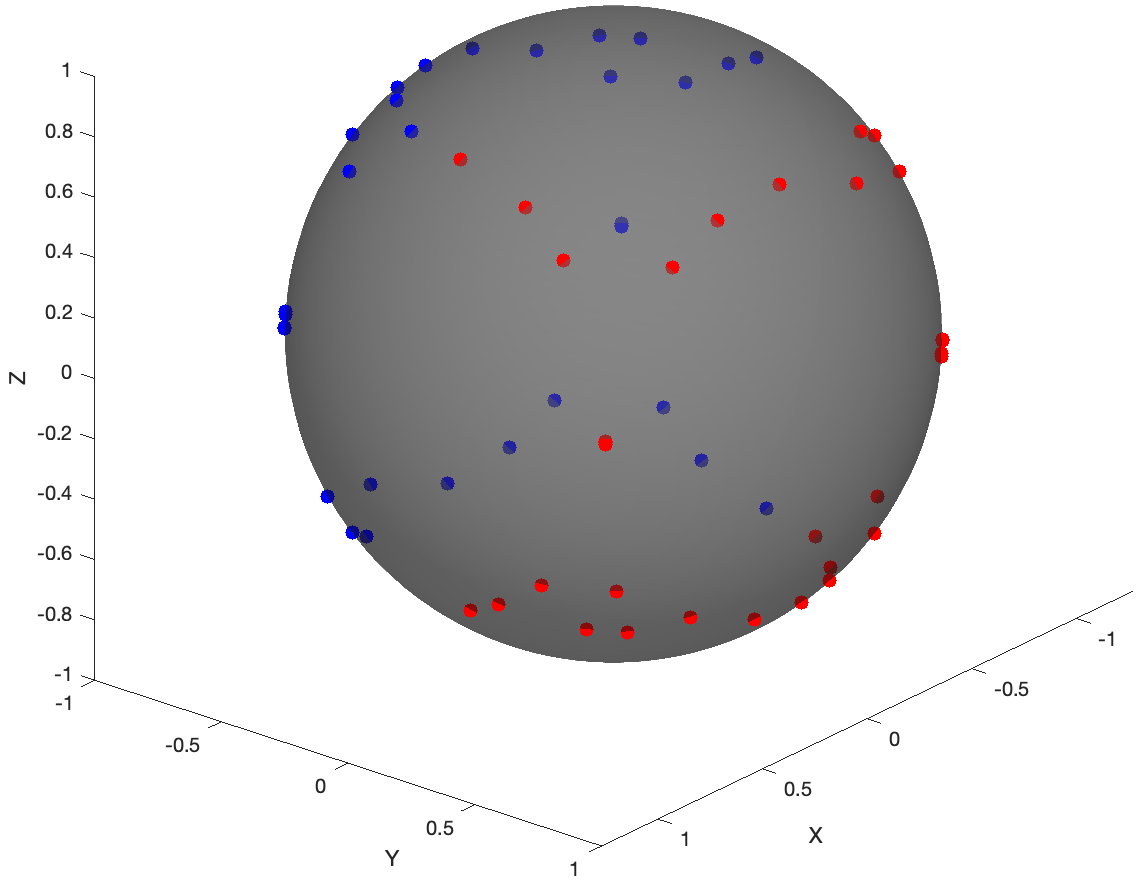
\includegraphics[width=.4\linewidth, angle=0]{figs/Overplus_VS_ISMRM/shell_overplus.png}}    
    \hfill
    \subfloat[Esquema utilizado no ISMRM.]{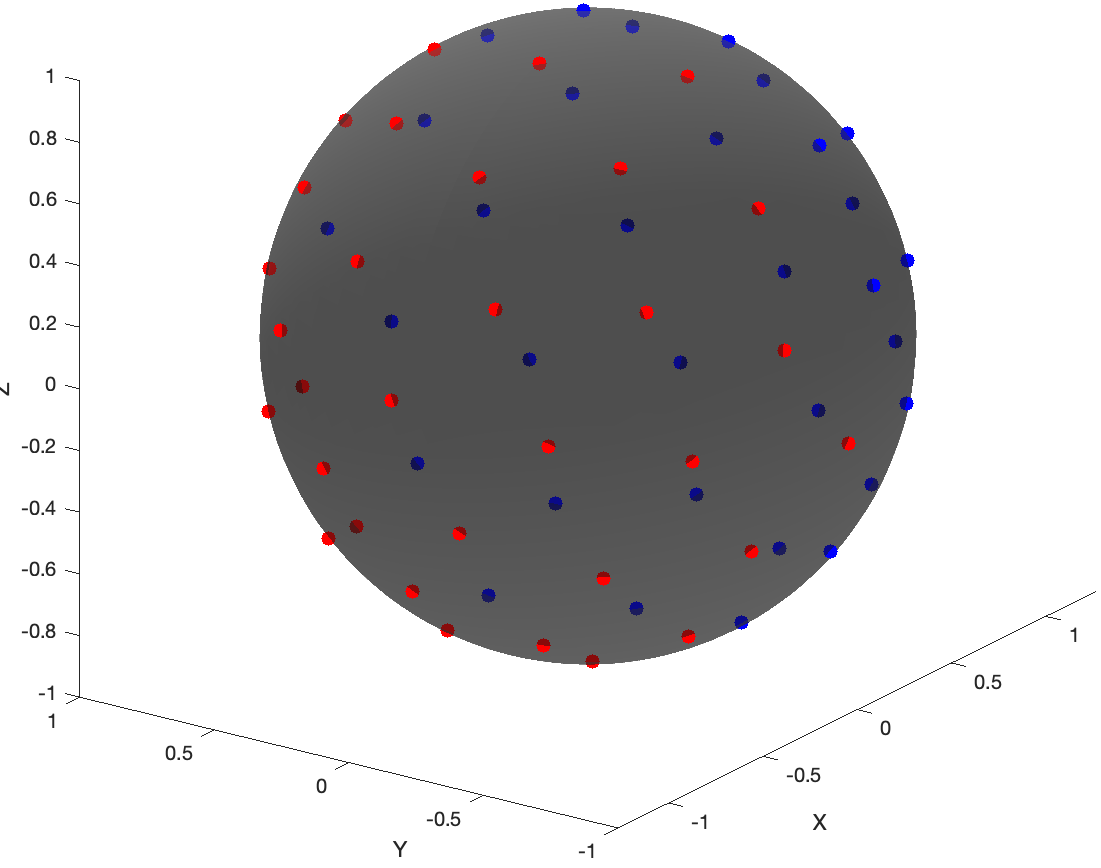
\includegraphics[width=.4\linewidth, angle=0]{figs/Overplus_VS_ISMRM/shell_ismrm.png}}
     \caption{Domínio esférico com pontos de amostragem referentes a direção de gradientes de difusão. Vermelho: direções de amostragem. Azul: sentido oposto da direção de amostragem.}
    %\hfill
    \label{fig::shell_Overplus_VS_ISMRM}
\end{figure}


Um bom conjunto de gradientes de codificação de difusão vinculada a um DWI não tem uma preferência direcional, as amostras no domínio esférico possuem uma boa invariância à orientação das estruturas do tecido ou coordenadas da máquina e a separação angular entre um par de pontos mais próximos é máxima e constante para todos os elementos \cite{cheng2018}. Um conjunto que segue essas propriedades estão distribuídos uniformemente sobre o \textit{shell}.

Há uma certa concordância na literatura de que uma uniformidade no domínio esférico em aquisições \textit{single shell}\footnote{Denomina-se aquisição \textit{single shell} como volumes de ressonância de difusão escaneados com apenas um valor b.} é importante para uma boa reconstrução de ODFs. \citeonline{yeh2010} mencionam a importância da uniformidade além de propor uma métrica para aferir o seu grau. \citeonline{cheng2018} discorrem sobre formulações de esquemas de amostragem de gradientes de forma uniforme e mencionam as suas vantagens.

Como parte do processo de investigação dos resultados não esperados de ODFs gerados a partir dos volumes adquiridos através do protocolo \textit{Overplus}, foram escaneados para um mesmo indivíduo um volume com o conjunto de direções da competição ISMRM, o padrão, e um usando o protocolo \textit{Overplus} da Philips, em que todos possuem a mesma resolução angular de 32 direções. A análise feita consistiu na inspeção da forma dos glifos na região do corpo caloso que contém uma forte componente na direção mediolateral. A localização desta região se dá através do mapa FA codificado por cor gerado pelo DTI, em que não foi constatado nenhum problema nestes esquemas de aquisição.


Nesta inspeção, foi possível gerar glifos das ODFs razoáveis para o esquema de amostragem do ISMRM (Figura \ref{fig::Overplus_VS_ISMRM_b}), o que não aconteceu com o \textit{Overplus}, em que as ODFs ficaram totalmente descaracterizadas em comparação com os códigos de cores, conforme mostrado na Figura \ref{fig::Overplus_VS_ISMRM_a}.

\begin{figure}[ht]
\centering
\captionsetup[subfloat]{farskip=5pt,nearskip=0pt}
    
    \subfloat[\textit{Overplus}] {\label{fig::Overplus_VS_ISMRM_a} 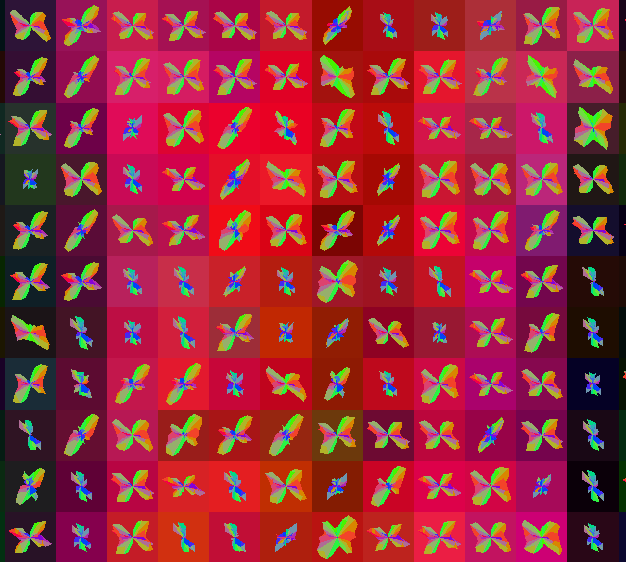
\includegraphics[width=.45\linewidth, angle=0, ]{figs/Overplus_VS_ISMRM/Overplus.png}}
    \hfill
    \subfloat[Esquema da competição ISMRM]{\label{fig::Overplus_VS_ISMRM_b} \includegraphics[width=.47\linewidth, angle=0]{figs/Overplus_VS_ISMRM/ISMRM.png}}
    %\hfill
    \caption{Glifos do Corpo Caloso - Mediolateral. Glifos de ODF sobre mapa FA codificado por cor do DTI.} %!!VER SE ISSO TA CERTO
    \label{fig::Overplus_VS_ISMRM}
\end{figure}
\pagebreak


%\bibliographystyle{}
\bibliography{references.bib}

% ----------------------------------------------------------
% Glossário
% ----------------------------------------------------------
%
% Consulte o manual da classe abntex2 para orientações sobre o glossário.
%
%\glossary

% ----------------------------------------------------------
% Apêndices
% ----------------------------------------------------------

% ---
% Inicia os apêndices
% ---
%\begin{apendicesenv}
%\end{apendicesenv}
% ---


% ----------------------------------------------------------
% Anexos
% ----------------------------------------------------------

% ---
% Inicia os anexos
% ---
\begin{anexosenv}
\end{anexosenv}

%---------------------------------------------------------------------
% INDICE REMISSIVO
%---------------------------------------------------------------------
%\phantompart
\printindex
%---------------------------------------------------------------------

\end{document}


